%% ============================================================================
%%  CAPITOLO 9 — Integrali indefiniti
%%  Fonte principale per argomenti e dimostrazioni: Marcellini–Sbordone, cap. 9
%%  (§67 teorema fondamentale del calcolo integrale; §68 primitive, formula
%%  fondamentale; §69 l'integrale indefinito; §70 integrazione per decomposizione
%%  in somma; §71 funzioni razionali; §72 integrazione per parti; §73 integrazione
%%  per sostituzione; §74 calcolo di aree di figure piane; appendice: §75 integrali
%%  impropri; §76 definizione di logaritmo, esponenziale, potenza).
%% ============================================================================
\aperturacapitolo{Integrali indefiniti}{cap:integrali-indefiniti}

\epigraph{Data aequatione quotcunque fluentes quantitates involvente, fluxiones
invenire; et vice versa.\\[2pt]
\upshape(Data un'equazione che contenga un numero qualsiasi di quantità fluenti,
trovarne le flussioni; e viceversa.)}{Isaac Newton, soluzione dell'anagramma inviato a
Leibniz nell'\emph{Epistola posterior} (1676)}

\lettrine[lines=3, findent=2pt, nindent=0pt]{N}{el capitolo precedente} abbiamo
definito l'integrale come elemento separatore tra somme inferiori e superiori, e lo
abbiamo calcolato con fatica in pochissimi casi: $x$, $x^{2}$, $x^{3}$, $2^{x}$, sempre
ricorrendo a formule ad hoc per le somme. Avevamo però notato una curiosa
coincidenza: la derivata dell'area $\frac{b^{3}}3$ del settore di parabola, pensata
come funzione dell'estremo $b$, è proprio $b^{2}$, il valore della funzione integranda.
In questo capitolo trasformiamo la coincidenza in un teorema, il \emph{teorema
fondamentale del calcolo integrale}: integrazione e derivazione sono operazioni
inverse l'una dell'altra. È la scoperta di Newton e di Leibniz che ha dato origine al
calcolo infinitesimale, e la sua conseguenza pratica è enorme: per calcolare
$\int_{a}^{b}f(x)\,dx$ basta conoscere una funzione $G$ la cui derivata sia $f$, cioè
una \emph{primitiva} di $f$, e calcolare $G(b)-G(a)$.

Il problema del calcolo degli integrali diventa così quello della ricerca delle
primitive, cioè degli \emph{integrali indefiniti}. Leggendo «al contrario» le regole di
derivazione otterremo gli integrali immediati e i tre metodi generali di integrazione:
per decomposizione in somma, per parti, per sostituzione, insieme a un procedimento
sistematico per le funzioni razionali. Li applicheremo al calcolo di aree, tra cui
quella del cerchio e dell'ellisse (verificando ciò che avevamo ammesso nel
\cref{cap:integrali-definiti}), e a un problema centrale delle costruzioni aeronautiche:
il taglio e il momento flettente lungo l'apertura di un'ala. Nelle appendici
estenderemo l'integrale agli intervalli illimitati e alle funzioni non limitate, e
mostreremo come il logaritmo, e con esso l'esponenziale e le potenze, si possa
\emph{definire} mediante un integrale. Seguiremo il testo di riferimento
\cite{marcellini-sbordone}.

\medskip
\noindent\textbf{In questo capitolo.}
\begin{itemize}
  \item La funzione integrale e il teorema fondamentale del calcolo integrale
  (\S\ref{sec:teorema-fondamentale}).
  \item Primitive e formula fondamentale del calcolo integrale (\S\ref{sec:primitive}).
  \item Approfondimento: la formula fondamentale per le funzioni regolari a tratti
  (\S\ref{subsec:regolari-tratti}).
  \item L'integrale indefinito, gli integrali immediati, la decomposizione in somma
  (\S\ref{sec:integrale-indefinito}).
  \item L'integrazione delle funzioni razionali (\S\ref{sec:razionali}).
  \item L'integrazione per parti (\S\ref{sec:per-parti}).
  \item L'integrazione per sostituzione (\S\ref{sec:sostituzione}).
  \item Approfondimento: le sostituzioni standard per le funzioni razionali di $\sen x$ e
  $\cos x$ e di $x$ e $\sqrt{x^{2}+a}$ (\S\ref{subsec:sostituzioni-standard}).
  \item Aree di figure piane e applicazioni: cerchio, ellisse, spazio percorso, taglio e
  momento flettente in un'ala (\S\ref{sec:applicazioni-integrali}).
  \item Appendice: integrali impropri (\S\ref{sec:impropri}).
  \item Approfondimento: un integrale convergente ma non assolutamente convergente
  (\S\ref{subsec:seno-su-x}).
  \item Appendice: logaritmo, esponenziale e potenza definiti mediante un integrale
  (\S\ref{sec:logaritmo-integrale}).
  \item Esercizi di riepilogo (\S\ref{sec:esercizi-cap9}).
  \item Punti fondamentali del capitolo (\S\ref{sec:sintesi-cap09}).
\end{itemize}

%% ----------------------------------------------------------------------------
%%  §9.1  Il teorema fondamentale del calcolo integrale
%% ----------------------------------------------------------------------------
\section{Il teorema fondamentale del calcolo integrale}
\label{sec:teorema-fondamentale}

Ci proponiamo di mettere in evidenza una relazione tra integrali e derivate che avrà
applicazioni in tutto il calcolo integrale. L'idea è di far variare uno degli estremi
di integrazione e di studiare l'integrale come \emph{funzione} di tale estremo.

\subsection{La funzione integrale}

Sia $f$ una funzione integrabile nell'intervallo $[a,b]$. Per il
\cref{lem:sottointervallo}, $f$ è integrabile in ogni intervallo $[a,x]$ con
$x\in[a,b]$, e possiamo considerare
\begin{equation}\label{eq:funzione-integrale}
  F(x)=\int_{a}^{x}f(t)\,dt, \qquad x\in[a,b] ,
\end{equation}
con $F(a)=0$ per la convenzione \eqref{eq:estremi-invertiti}. Abbiamo indicato la
variabile di integrazione con $t$ invece che con $x$: è un puro scambio di simboli,
perché la variabile di integrazione è muta, ma ci permette di riservare la lettera $x$
al secondo estremo. Per ogni $x$ l'integrale è un numero, e al variare di $x$ si ottiene
una funzione, detta \emph{funzione integrale} di $f$ con punto iniziale
$a$.\index{funzione!integrale} Ad esempio, per le \eqref{eq:integrale-x} e
\eqref{eq:integrale-x2},
\begin{equation}\label{eq:funzioni-integrali-esempi}
  \int_{0}^{x}t\,dt=\frac{x^{2}}2, \qquad \int_{0}^{x}t^{2}\,dt=\frac{x^{3}}3
  \qquad (x\ge0) .
\end{equation}
In entrambi i casi la derivata della funzione integrale ($x$ e $x^{2}$) è la funzione
integranda calcolata nel secondo estremo. È il fenomeno osservato
nell'\cref{oss:indizio-tfc}; vedremo che vale in generale.

Se si sceglie un altro punto iniziale $c\in[a,b]$, per l'additività
(\cref{teo:additivita}) si ha $\int_{c}^{x}f=\int_{a}^{x}f-\int_{a}^{c}f=F(x)-F(c)$: le
funzioni integrali con punti iniziali diversi differiscono per una costante.

\begin{proposizione}[La funzione integrale è lipschitziana]\label{prop:integrale-lipschitz}
Sia $f$ integrabile in $[a,b]$, con $\abs{f(t)}\le K$ per ogni $t\in[a,b]$. Allora
\begin{equation}\label{eq:integrale-lipschitz}
  \abs{F(x)-F(x')}\le K\,\abs{x-x'} \qquad\perogni x,x'\in[a,b] ;
\end{equation}
in particolare $F$ è uniformemente continua in $[a,b]$.
\end{proposizione}

\begin{schema}
\Ipotesi{$f$ integrabile in $[a,b]$; \ $\abs f\le K$.}
\Tesi{$F$ lipschitziana con costante $K$, e quindi uniformemente continua.}
\end{schema}

\begin{strategia}
Per l'additività, $F(x)-F(x')$ è l'integrale di $f$ tra $x'$ e $x$; lo si stima con il
valore assoluto e il confronto con la costante $K$.
\end{strategia}

\begin{dimostrazione}
Siano $x'<x$ (se $x=x'$ non c'è nulla da dimostrare, e il caso $x<x'$ è simmetrico).
Per l'additività, $F(x)-F(x')=\int_{x'}^{x}f(t)\,dt$, e per il \cref{teo:valore-assoluto}
e il \cref{teo:confronto-integrali},
\[
  \abs{F(x)-F(x')}\le\int_{x'}^{x}\abs{f(t)}\,dt\le\int_{x'}^{x}K\,dt=K\,(x-x') .
\]
L'uniforme continuità segue dalla \cref{prop:lipschitz-uniforme}.
\end{dimostrazione}

La funzione integrale è dunque sempre continua, anche quando $f$ non lo è; ma può non
essere derivabile. Ad esempio, se in $[-1,1]$ si pone $f(t)=-1$ per $t<0$ e $f(t)=1$ per
$t\ge0$, si trova $\int_{-1}^{x}f(t)\,dt=-(x+1)$ per $x\le0$ e $-1+x$ per $x\ge0$ (il
valore di $f$ nel solo punto $0$ non conta, per l'\cref{es:valore-in-un-punto}),
cioè $F(x)=\abs x-1$, che non è derivabile in $0$: il salto della funzione integranda
diventa un punto angoloso della funzione integrale. Il teorema seguente afferma che,
dove $f$ è continua, $F$ è derivabile.

\subsection{Il teorema fondamentale}

\begin{teorema}[fondamentale del calcolo integrale]\label{teo:fondamentale}
\index{teorema!fondamentale del calcolo integrale}
Sia $f$ una funzione continua nell'intervallo $[a,b]$. La funzione integrale
\eqref{eq:funzione-integrale} è derivabile in $[a,b]$ e la sua derivata vale
\begin{equation}\label{eq:teorema-fondamentale}
  F'(x)=f(x) \qquad\perogni x\in[a,b]
\end{equation}
(negli estremi $a$ e $b$ si intendono la derivata destra e la derivata sinistra).
\end{teorema}

\begin{schema}
\Ipotesi{$f$ continua in $[a,b]$; \ $F(x)=\int_{a}^{x}f(t)\,dt$.}
\Tesi{$F$ derivabile in $[a,b]$ e $F'(x)=f(x)$ per ogni $x$.}
\end{schema}

\begin{strategia}
Dobbiamo calcolare il limite del rapporto incrementale di $F$. Per l'additività,
l'incremento $F(x+h)-F(x)$ è l'integrale di $f$ tra $x$ e $x+h$, e il rapporto
incrementale è quindi la \emph{media integrale} di $f$ sull'intervallo di estremi $x$ e
$x+h$. Il teorema della media la trasforma in un valore $f(\xi_{h})$, con $\xi_{h}$ compreso
tra $x$ e $x+h$; quando $h\to0$ il punto $\xi_{h}$ è costretto a tendere a $x$, e la
continuità di $f$ in $x$ fa il resto. Geometricamente: la striscia di base $h$ aggiunta
al rettangoloide ha un'area molto vicina a quella del rettangolo di altezza $f(x)$.
\end{strategia}

\begin{dimostrazione}
Sia $x\in[a,b]$ e sia $h\neq0$ tale che $x+h\in[a,b]$. Per l'additività
(\cref{teo:additivita}),
\begin{equation}\label{eq:rapporto-funzione-integrale}
  \frac{F(x+h)-F(x)}h=\frac1h\Bigl[\int_{a}^{x+h}f(t)\,dt-\int_{a}^{x}f(t)\,dt\Bigr]
  =\frac1h\int_{x}^{x+h}f(t)\,dt .
\end{equation}
Se $h>0$, l'ultimo membro è la media integrale di $f$ in $[x,x+h]$; se $h<0$, per la
\eqref{eq:estremi-invertiti} esso vale $\frac1{\abs h}\int_{x+h}^{x}f(t)\,dt$, cioè la media
integrale di $f$ in $[x+h,x]$. In entrambi i casi, per il teorema della media
(\cref{teo:media}) applicato alla funzione continua $f$, esiste un punto $\xi_{h}$
dell'intervallo di estremi $x$ e $x+h$ tale che
\begin{equation}\label{eq:rapporto-media}
  \frac{F(x+h)-F(x)}h=f(\xi_{h}), \qquad \abs{\xi_{h}-x}\le\abs h .
\end{equation}
Sia ora $\epsilon>0$. Per la continuità di $f$ in $x$ esiste $\delta>0$ tale che
$\abs{f(t)-f(x)}<\epsilon$ per ogni $t\in[a,b]$ con $\abs{t-x}<\delta$. Se $0<\abs h<\delta$,
allora $\abs{\xi_{h}-x}\le\abs h<\delta$, e quindi
\[
  \Bigl|\frac{F(x+h)-F(x)}h-f(x)\Bigr|=\abs{f(\xi_{h})-f(x)}<\epsilon .
\]
Questo prova che il rapporto incrementale tende a $f(x)$ per $h\to0$ (soltanto da destra
se $x=a$, soltanto da sinistra se $x=b$), cioè la \eqref{eq:teorema-fondamentale}.
\end{dimostrazione}

\begin{figure}[htb]
\centering
\begin{tikzpicture}
\begin{axis}[name=t1, width=0.5\textwidth, height=4.6cm, axis lines=left, xmin=0,
  xmax=4.4, ymin=0, ymax=2.5, xtick={0.5,2.6}, xticklabels={$a$,$x$}, ytick=\empty,
  title={\scriptsize $F(x)$ = area da $a$ a $x$}, clip=false]
  \addplot[draw=none, fill=blu!22, domain=0.5:2.6, samples=50]
    {1.1+0.6*sin(deg(1.3*x))+0.1*x} \closedcycle;
  \addplot[curva, domain=0.3:4.2, samples=100] {1.1+0.6*sin(deg(1.3*x))+0.1*x};
  \node[font=\scriptsize, blu] at (axis cs:1.55,0.6) {$F(x)$};
  \node[font=\scriptsize] at (axis cs:3.7,1.45) {$y=f(t)$};
\end{axis}
\begin{axis}[at={(t1.east)}, anchor=west, xshift=0.7cm, width=0.5\textwidth,
  height=4.6cm, axis lines=left, xmin=0, xmax=4.4, ymin=0, ymax=2.5,
  xtick={2.6,3.2}, xticklabels={$x$,$x+h$}, ytick={1.2183},
  yticklabels={$f(x)$}, title={\scriptsize l'incremento $F(x+h)-F(x)$},
  tick label style={font=\scriptsize}]
  \addplot[draw=none, fill=rame!35, domain=2.6:3.2, samples=30]
    {1.1+0.6*sin(deg(1.3*x))+0.1*x} \closedcycle;
  \draw[blu, thick] (axis cs:2.6,0) rectangle (axis cs:3.2,1.2183);
  \addplot[curva, domain=0.3:4.2, samples=100] {1.1+0.6*sin(deg(1.3*x))+0.1*x};
  \addplot[tratteggio] coordinates {(0,1.2183) (2.6,1.2183)};
\end{axis}
\end{tikzpicture}
\caption{A sinistra, la funzione integrale $F(x)$ come area del rettangoloide da $a$ a
$x$. A destra, l'incremento $F(x+h)-F(x)$ è l'area della striscia in color rame, che
differisce poco da quella del rettangolo $f(x)\,h$ (contorno blu): dividendo per $h$ e
facendo tendere $h$ a zero si ottiene $F'(x)=f(x)$.}
\label{fig:teorema-fondamentale}
\end{figure}

La dimostrazione usa la continuità di $f$ soltanto nel punto $x$ (oltre che per poter
applicare il teorema della media). In effetti vale un risultato più generale, che spiega
il punto angoloso dell'esempio precedente.

\begin{osservazione}[Basta la continuità nel punto]\label{oss:fondamentale-puntuale}
Sia $f$ integrabile in $[a,b]$ e continua in un punto $x_{0}$. Allora $F$ è derivabile
in $x_{0}$ e $F'(x_{0})=f(x_{0})$. Infatti, poiché $\frac1h\int_{x_{0}}^{x_{0}+h}f(x_{0})\,dt
=f(x_{0})$, dalla \eqref{eq:rapporto-funzione-integrale} si ha
\[
  \frac{F(x_{0}+h)-F(x_{0})}h-f(x_{0})=\frac1h\int_{x_{0}}^{x_{0}+h}\bigl[f(t)-f(x_{0})\bigr]dt ,
\]
e se $\abs{f(t)-f(x_{0})}<\epsilon$ per $\abs{t-x_{0}}<\delta$, per $0<\abs h<\delta$ il secondo
membro non supera in valore assoluto $\frac1{\abs h}\,\epsilon\abs h=\epsilon$ (per il
\cref{teo:valore-assoluto} e il confronto). Dove $f$ ha un salto, invece, i rapporti
incrementali destro e sinistro di $F$ tendono ai due limiti laterali di $f$ (con lo
stesso argomento, usando i limiti laterali al posto di $f(x_{0})$), e $F$ ha un punto
angoloso.
\end{osservazione}

Il teorema fondamentale si combina con la regola di derivazione delle funzioni composte.

\begin{corollario}[Estremi variabili]\label{cor:estremi-variabili}
Sia $f$ continua in un intervallo $I$, siano $c\in I$ e $\varphi$ una funzione
derivabile in un intervallo $J$, con valori in $I$. Allora, rispettivamente per ogni
$x\in I$ e per ogni $x\in J$,
\begin{equation}\label{eq:estremi-variabili}
  \frac{d}{dx}\int_{x}^{c}f(t)\,dt=-f(x), \qquad
  \frac{d}{dx}\int_{c}^{\varphi(x)}f(t)\,dt=f\bigl(\varphi(x)\bigr)\,\varphi'(x) .
\end{equation}
\end{corollario}

\begin{schema}
\Ipotesi{$f$ continua nell'intervallo $I$; \ $c\in I$; \ $\varphi:J\to I$ derivabile
($J$ intervallo).}
\Tesi{le due formule \eqref{eq:estremi-variabili}.}
\end{schema}

\begin{strategia}
Con $F(x)=\int_{c}^{x}f$ si ha $\int_{x}^{c}f=-F(x)$ e $\int_{c}^{\varphi(x)}f=F(\varphi(x))$;
basta derivare con il teorema fondamentale e la regola della catena.
\end{strategia}

\begin{dimostrazione}
Sia $F(x)=\int_{c}^{x}f(t)\,dt$. Per la \eqref{eq:estremi-invertiti},
$\int_{x}^{c}f=-F(x)$, la cui derivata è $-f(x)$ per il \cref{teo:fondamentale} (applicato
in un intervallo chiuso e limitato contenuto in $I$ che contenga $c$ e $x$, con $x$ al suo
interno se $x$ non è un estremo di $I$). Inoltre
$\int_{c}^{\varphi(x)}f=F(\varphi(x))$, e per il \cref{teo:derivata-composta} la sua derivata
è $F'(\varphi(x))\,\varphi'(x)=f(\varphi(x))\,\varphi'(x)$.
\end{dimostrazione}

Ad esempio, $\frac{d}{dx}\int_{0}^{x^{2}}e^{-t^{2}}dt=2x\,e^{-x^{4}}$: la derivata si calcola
senza conoscere alcuna formula esplicita per l'integrale. È proprio questo il punto di
forza del teorema: la funzione $\int_{0}^{x}e^{-t^{2}}dt$, che non si esprime mediante
funzioni elementari, ha comunque derivata nota, ed è quindi crescente, con un flesso
nell'origine, dove $e^{-x^{2}}$ ha il massimo (\cref{fig:funzione-integrale}). Il programma
seguente calcola numericamente la funzione integrale e ne verifica la derivata con il
rapporto incrementale simmetrico; come riferimento usa la funzione \texttt{erf} di Python,
definita proprio come $\frac2{\sqrt\pi}\int_{0}^{x}e^{-t^{2}}dt$.

\begin{python}[La funzione integrale di $e^{-t^2}$ e la sua derivata]
import math

f = lambda t: math.exp(-t * t)

def F(x, n=2000):
    """Funzione integrale int_0^x f(t) dt (punto medio)."""
    h = x / n
    return h * sum(f((k + 0.5) * h) for k in range(n))

h = 1e-3
print("  x      F(x)  sqrt(pi)/2 erf(x)   rapp. incr.     f(x)")
for x in (0.0, 0.5, 1.0, 1.5, 2.0):
    rif = math.sqrt(math.pi) / 2 * math.erf(x)
    d = (F(x + h) - F(x - h)) / (2 * h)
    print(f"{x:4.1f}  {F(x):.6f}      {rif:.6f}      {d:.6f}"
          f"   {f(x):.6f}")
\end{python}
\begin{risultato}
  x      F(x)  sqrt(pi)/2 erf(x)   rapp. incr.     f(x)
 0.0  0.000000      0.000000      1.000000   1.000000
 0.5  0.461281      0.461281      0.778801   0.778801
 1.0  0.746824      0.746824      0.367880   0.367879
 1.5  0.856188      0.856188      0.105399   0.105399
 2.0  0.882081      0.882081      0.018316   0.018316
\end{risultato}

\begin{figure}[htb]
\centering
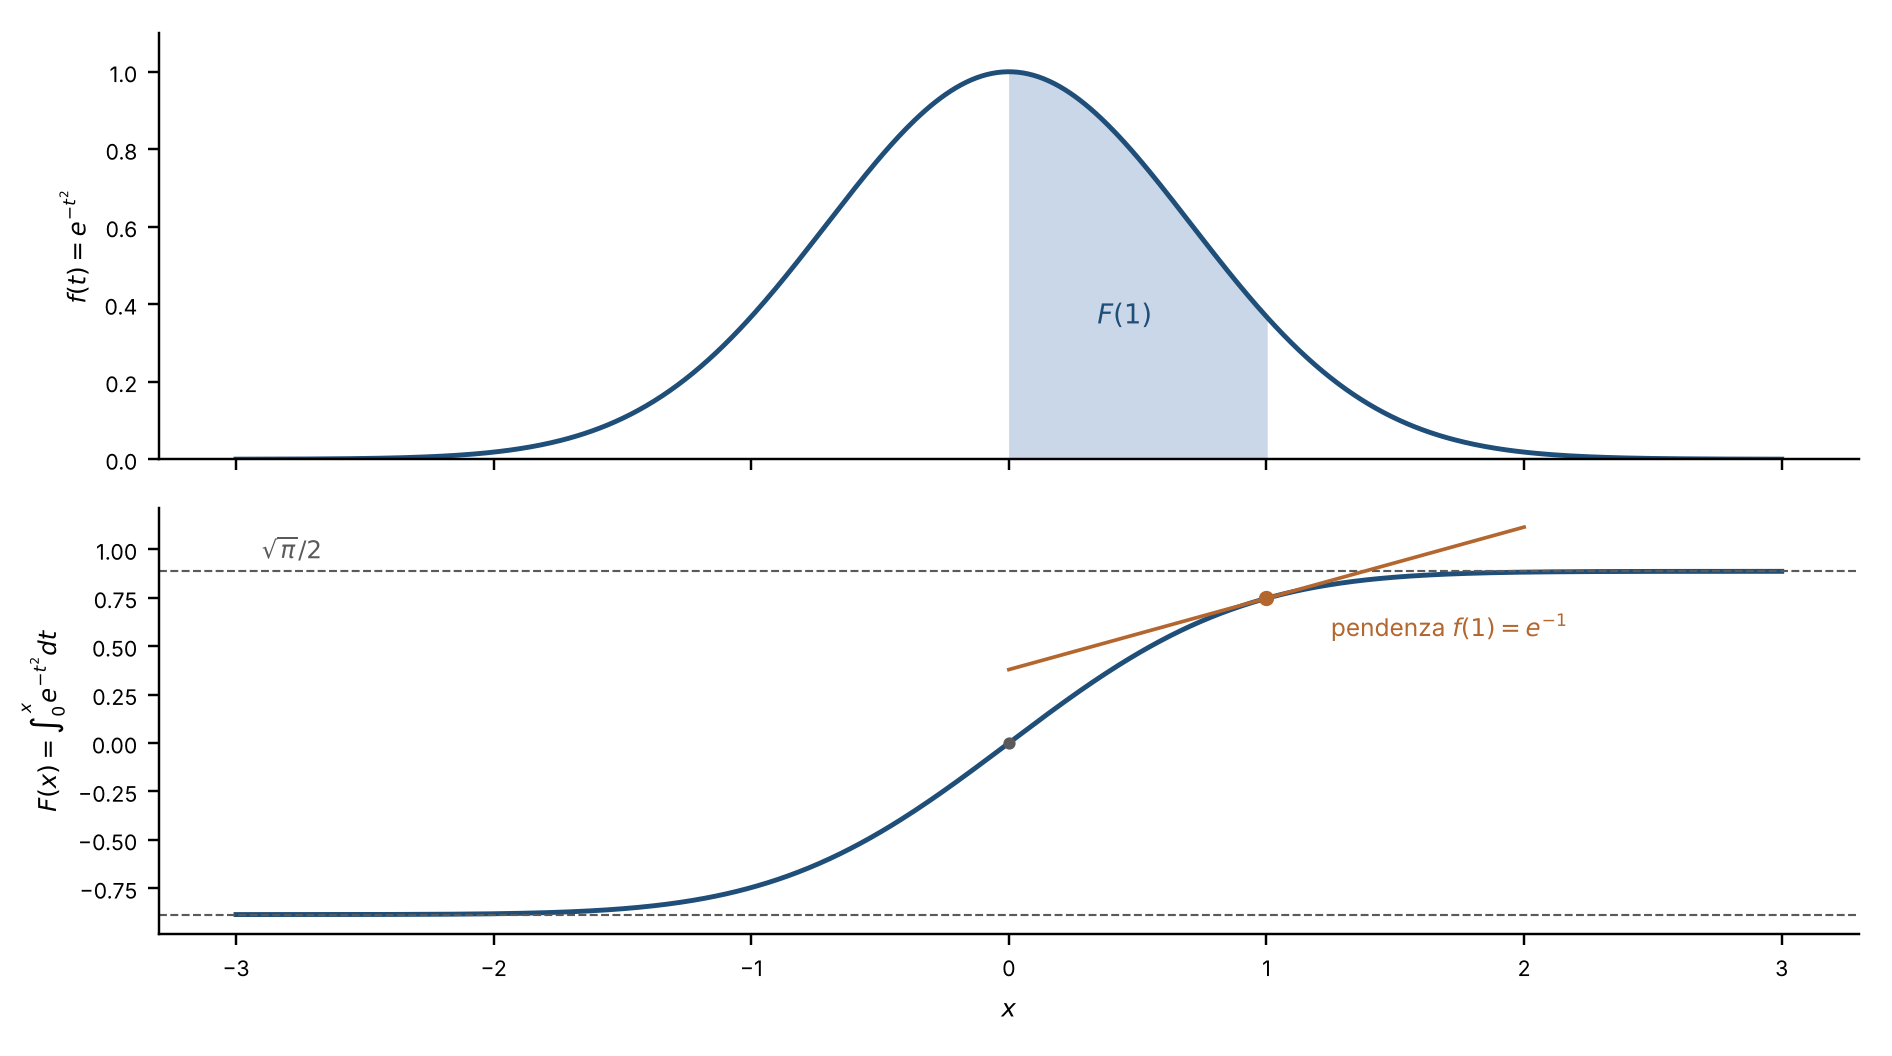
\includegraphics[width=\textwidth]{figure/funzione_integrale.png}
\caption{In alto, la funzione $f(t)=e^{-t^{2}}$ con l'area da $0$ a $x=1$; in basso, la
sua funzione integrale $F(x)=\int_{0}^{x}e^{-t^{2}}dt$, con la retta tangente in $x=1$, di
pendenza $f(1)=e^{-1}$. Dove $f$ è massima, $F$ ha il flesso; l'esistenza degli asintoti
orizzontali sarà dimostrata nel \cref{sec:impropri}, mentre il loro valore $\pm\frac{\sqrt\pi}2$ si
calcola in un corso di Analisi Matematica~2
(\texttt{python/fig\_funzione\_integrale.py}).}
\label{fig:funzione-integrale}
\end{figure}

\begin{notastorica}[Newton, Leibniz e la disputa sulla priorità]
Il legame tra il problema delle tangenti e quello delle aree fu intravisto da diversi
matematici del Seicento: Evangelista Torricelli, James Gregory e soprattutto Isaac
Barrow, che nelle \emph{Lectiones geometricae} (1670) ne diede una formulazione
geometrica. Furono però Isaac Newton, intorno al 1665--1666, e Gottfried Wilhelm
Leibniz, a Parigi, intorno al 1675, a farne lo strumento di un calcolo generale, con
notazioni e regole valide per tutte le curve (Newton, nel 1669, succedette proprio a
Barrow sulla cattedra lucasiana di Cambridge). Nello stesso 1669 Newton raccolse i suoi
metodi nel \emph{De analysi}, stampato soltanto nel 1711: vi mostrava che l'area sotto
una curva, pensata come funzione dell'ascissa, cresce con velocità uguale all'ordinata
(il nostro $F'=f$), e calcolava le aree sviluppando in serie e integrando termine a
termine. Newton
comunicò il risultato a Leibniz in forma cifrata, con l'anagramma dell'epigrafe, nella
lettera del 24 ottobre 1676; Leibniz pubblicò per primo, nel 1684 e nel 1686, sugli
\emph{Acta Eruditorum}. Ne seguì una violenta disputa sulla priorità, che la Royal
Society, presieduta da Newton, chiuse nel 1712 a favore del suo presidente (il rapporto
fu pubblicato nel 1713 nel \emph{Commercium epistolicum}) e che divise
per un secolo i matematici inglesi da quelli del continente. Oggi si riconosce che le
due scoperte furono indipendenti. La parola «integrale» comparve a stampa nel 1690, in
una memoria di Jakob Bernoulli sugli \emph{Acta Eruditorum}; Leibniz, che parlava di
\emph{calculus summatorius}, adottò poi il nome \emph{calculus integralis} proposto da
Johann Bernoulli. La dimostrazione rigorosa che abbiamo seguito, basata sul teorema
della media, è dovuta a Cauchy (1823). Avendo definito l'integrale come limite di somme
(si veda la nota storica del \S\ref{sec:integrale-definito}), Cauchy dovette
\emph{dimostrare} ciò che per i predecessori, per i quali integrare significava trovare
una primitiva, era quasi una definizione.
\end{notastorica}

%% ----------------------------------------------------------------------------
%%  §9.2  Primitive. Formula fondamentale del calcolo integrale
%% ----------------------------------------------------------------------------
\section{Primitive. Formula fondamentale del calcolo integrale}
\label{sec:primitive}

\begin{definizione}[Primitiva]\label{def:primitiva}\index{primitiva}
Sia $f$ una funzione definita in un intervallo $I$. Una funzione $F$ si dice una
\emph{primitiva} di $f$ in $I$ se $F$ è derivabile in $I$ e $F'(x)=f(x)$ per ogni $x\in I$.
\end{definizione}

Ad esempio, una primitiva di $f(x)=x$ in $\R$ è $F(x)=\frac{x^{2}}2$; una primitiva di
$\sen x$ è $-\cos x$; una primitiva di $\frac1x$ nell'intervallo $(0,+\infty)$ è $\log x$.
Con la definizione di primitiva, il teorema fondamentale si enuncia così: \emph{se $f$ è
continua in $[a,b]$, la funzione integrale $F(x)=\int_{a}^{x}f(t)\,dt$ è una primitiva di
$f$}. Più in generale, se $f$ è continua in un intervallo $I$ qualsiasi (aperto,
semiaperto o illimitato) e $c\in I$, la funzione $\int_{c}^{x}f(t)\,dt$ è una primitiva di
$f$ in $I$: basta applicare il \cref{teo:fondamentale} in un intervallo chiuso e
limitato contenuto in $I$ che contenga $c$ e il punto $x$ considerato, con $x$ al suo
interno se $x$ non è un estremo di $I$. Dunque:

\begin{center}
\emph{ogni funzione continua in un intervallo ammette primitive.}
\end{center}

Non tutte le funzioni, però, ammettono primitive, neppure se sono integrabili. La
funzione $f$ che vale $-1$ per $x<0$ e $1$ per $x\ge0$ è integrabile in $[-1,1]$, ma non ha
primitive: se fosse $G'=f$ in $[-1,1]$, la derivata $G'$ non si annullerebbe mai e
cambierebbe segno, contro il lemma di Darboux (\cref{lem:darboux}). Viceversa, esistono
funzioni discontinue che ammettono primitive, come la derivata di $x^{2}\sen\frac1x$
(\cref{oss:f2-non-C1}).

\subsection{Le primitive di una funzione in un intervallo}

Se $F$ è una primitiva di $f$, anche $F+c$ lo è, qualunque sia la costante $c$, perché la
derivata di una costante è nulla. Il teorema seguente afferma che in un intervallo non
ce ne sono altre.

\begin{teorema}[Caratterizzazione delle primitive in un intervallo]
\label{teo:caratterizzazione-primitive}
Se $F$ e $G$ sono due primitive di una stessa funzione $f$ in un intervallo $I$, esiste
una costante $c$ tale che
\begin{equation}\label{eq:primitive-costante}
  G(x)=F(x)+c \qquad\perogni x\in I .
\end{equation}
\end{teorema}

\begin{schema}
\Ipotesi{$I$ intervallo; \ $F'=G'=f$ in $I$.}
\Tesi{$G-F$ è costante in $I$.}
\end{schema}

\begin{strategia}
La differenza $H=G-F$ ha derivata nulla in $I$. Una funzione con derivata nulla in un
intervallo è costante: è una conseguenza del teorema di Lagrange, già dimostrata nel
\cref{cap:applicazioni-derivate}. L'ipotesi che $I$ sia un intervallo serve proprio a
poter applicare il teorema di Lagrange tra due punti qualsiasi.
\end{strategia}

\begin{dimostrazione}
Sia $H=G-F$; allora $H$ è derivabile in $I$ e $H'(x)=G'(x)-F'(x)=f(x)-f(x)=0$ per ogni
$x\in I$. Fissato $x_{0}\in I$, sia $x\in I$ con $x\neq x_{0}$. Poiché $I$ è un intervallo,
contiene l'intervallo chiuso di estremi $x_{0}$ e $x$, nel quale $H$ è continua (perché
derivabile) con derivata nulla; per il \cref{cor:funzioni-costanti}, $H$ è costante in
tale intervallo, e quindi $H(x)=H(x_{0})$. Posto $c=H(x_{0})$, si ha $G(x)=F(x)+c$ per ogni
$x\in I$.
\end{dimostrazione}

L'ipotesi che il dominio sia un intervallo è essenziale. Le funzioni $F(x)=\log\abs x$ e
\[
  G(x)=\begin{cases} \log\abs x+1 & \text{se } x>0,\\ \log\abs x+2 & \text{se } x<0 \end{cases}
\]
hanno entrambe derivata $\frac1x$ in $\R\setminus\set{0}$ (lo verificheremo nella
\eqref{eq:derivata-log-abs}), ma la loro differenza non è costante: su ciascuno dei due
intervalli $(-\infty,0)$ e $(0,+\infty)$ la costante può essere scelta indipendentemente.

\begin{figure}[htb]
\centering
\begin{tikzpicture}
\begin{axis}[name=p1, width=0.52\textwidth, height=5cm, axis lines=middle,
  xmin=-0.4, xmax=6.6, ymin=-2.3, ymax=3.4, xtick=\empty,
  ytick=\empty, title={\scriptsize primitive di $\cos x$: $\sen x+c$}, clip=false]
  \addplot[curva3, domain=-0.3:6.4, samples=100] {sin(deg(x))-1};
  \addplot[curva, domain=-0.3:6.4, samples=100] {sin(deg(x))};
  \addplot[curva2, domain=-0.3:6.4, samples=100] {sin(deg(x))+1};
  \addplot[curva3, domain=-0.3:6.4, samples=100] {sin(deg(x))+2};
  \addplot[tratteggio] coordinates {(1.2,-2.2) (1.2,3.3)};
  \addplot[grigio, thick] coordinates {(0.4,-0.358) (2.0,0.222)};
  \addplot[grigio, thick] coordinates {(0.4,0.642) (2.0,1.222)};
  \addplot[grigio, thick] coordinates {(0.4,1.642) (2.0,2.222)};
  \addplot[grigio, thick] coordinates {(0.4,2.642) (2.0,3.222)};
  \addplot[only marks, mark=*, mark size=1.1pt, grigio] coordinates
    {(1.2,-0.068) (1.2,0.932) (1.2,1.932) (1.2,2.932)};
  \node[font=\scriptsize, anchor=north] at (axis cs:1.2,-2.25) {$x_{0}$};
\end{axis}
\begin{axis}[at={(p1.east)}, anchor=west, xshift=0.7cm, width=0.46\textwidth,
  height=5cm, axis lines=middle, xmin=-0.3, xmax=3.6, ymin=-0.2, ymax=1.35,
  xtick={1.5708,3.1416}, xticklabels={$\frac\pi2$,$\pi$}, ytick={1},
  title={\scriptsize $\int_{0}^{\pi}\sen x\,dx=2$}]
  \addplot[draw=none, fill=blu!22, domain=0:3.1416, samples=60] {sin(deg(x))}
    \closedcycle;
  \addplot[curva, domain=0:3.1416, samples=80] {sin(deg(x))};
  \node[font=\scriptsize, blu] at (axis cs:1.5708,0.42) {area $=2$};
\end{axis}
\end{tikzpicture}
\caption{A sinistra, alcune primitive di $\cos x$: i loro grafici si ottengono l'uno
dall'altro per traslazione verticale, e nello stesso punto $x_{0}$ hanno tangenti
parallele, di pendenza $\cos x_{0}$. A destra, l'area sotto un arco di sinusoide, calcolata
con la formula fondamentale \eqref{eq:formula-fondamentale}.}
\label{fig:primitive}
\end{figure}

\subsection{La formula fondamentale}

Il risultato seguente riconduce il calcolo degli integrali definiti alla ricerca delle
primitive.

\begin{teorema}[Formula fondamentale del calcolo integrale]\label{teo:formula-fondamentale}
\index{formula fondamentale del calcolo integrale}
Sia $f$ una funzione continua in $[a,b]$ e sia $G$ una primitiva di $f$ in $[a,b]$. Allora
\begin{equation}\label{eq:formula-fondamentale}
  \int_{a}^{b}f(x)\,dx=\Bigl[G(x)\Bigr]_{a}^{b}=G(b)-G(a) .
\end{equation}
\end{teorema}

\begin{schema}
\Ipotesi{$f$ continua in $[a,b]$; \ $G'=f$ in $[a,b]$.}
\Tesi{$\int_{a}^{b}f=G(b)-G(a)$.}
\end{schema}

\begin{strategia}
La funzione integrale $F(x)=\int_{a}^{x}f$ è una primitiva di $f$ (teorema fondamentale),
come $G$. Per la caratterizzazione delle primitive, $G=F+c$; la costante si determina
calcolando in $x=a$, dove $F$ si annulla, e la tesi si ottiene calcolando in $x=b$.
\end{strategia}

\begin{dimostrazione}
Per il \cref{teo:fondamentale}, $F(x)=\int_{a}^{x}f(t)\,dt$ è una primitiva di $f$ in
$[a,b]$; per il \cref{teo:caratterizzazione-primitive} esiste una costante $c$ tale che
\[
  G(x)=F(x)+c=c+\int_{a}^{x}f(t)\,dt \qquad\perogni x\in[a,b] .
\]
Per $x=a$ si ottiene $G(a)=c+0=c$; sostituendo, $G(x)=G(a)+\int_{a}^{x}f(t)\,dt$, e per
$x=b$ si ha la tesi.
\end{dimostrazione}

Il simbolo $\bigl[G(x)\bigr]_{a}^{b}$ indica la differenza $G(b)-G(a)$; si scrive anche
$G(x)\big|_{a}^{b}$. La formula vale anche se $a>b$, per la \eqref{eq:estremi-invertiti}.

\begin{esempio}[Primi integrali calcolati con la formula fondamentale]
\label{es:formula-fondamentale}
Ecco alcuni integrali che il \cref{cap:integrali-definiti} non permetteva di calcolare, o
permetteva di calcolare soltanto con fatica.
\begin{enumerate}[label=\textup{(\alph*)}]
  \item Il settore di parabola: $G(x)=\frac{x^{3}}3$ è una primitiva di $x^{2}$, e
  \[
    \int_{0}^{b}x^{2}\,dx=\Bigl[\frac{x^{3}}3\Bigr]_{0}^{b}=\frac{b^{3}}3 .
  \]
  Il risultato di Archimede,
  che ci era costato un paragrafo, si ottiene in una riga.
  \item L'arco di sinusoide (\cref{fig:primitive}, a destra):
  $\int_{0}^{\pi}\sen x\,dx=\bigl[-\cos x\bigr]_{0}^{\pi}=-\cos\pi+\cos0=2$.
  \item Poiché $D\operatorname{arctg}x=\frac1{1+x^{2}}$ \eqref{eq:derivata-arctg},
  $\int_{0}^{1}\frac{dx}{1+x^{2}}=\operatorname{arctg}1-\operatorname{arctg}0=\frac\pi4$: è il
  valore annunciato negli esercizi del \cref{cap:integrali-definiti}, e quindi anche
  $\sum_{k=1}^{n}\frac n{n^{2}+k^{2}}\to\frac\pi4$ (\cref{es:limiti-riemann}).
  \item Poiché $D\,2^{x}=2^{x}\log2$ \eqref{eq:derivata-ax}, una primitiva di $2^{x}$ è
  $\frac{2^{x}}{\log2}$, e $\int_{0}^{1}2^{x}\,dx=\frac{2-1}{\log2}=\frac1{\log2}$, come avevamo
  trovato con le progressioni geometriche (\cref{es:integrale-esponenziale}).
\end{enumerate}
\end{esempio}

\begin{osservazione}[La formula fondamentale senza il teorema fondamentale]
\label{oss:formula-fondamentale-integrabili}
La formula \eqref{eq:formula-fondamentale} vale anche se $f$ è soltanto integrabile in
$[a,b]$, purché abbia una primitiva $G$ in $[a,b]$. Infatti, per ogni partizione
$P=\set{x_{0},\dots,x_{n}}$, il teorema di Lagrange applicato a $G$ in ciascun intervallo
$[x_{k-1},x_{k}]$ fornisce punti $\xi_{k}$ con $G(x_{k})-G(x_{k-1})=f(\xi_{k})\,\Delta x_{k}$, e
sommando (la somma a primo membro è telescopica)
\[
  G(b)-G(a)=\sum_{k=1}^{n}f(\xi_{k})\,\Delta x_{k} ,
\]
che è una somma di Riemann, compresa tra $s(P)$ e $S(P)$. Il numero $G(b)-G(a)$ è dunque un
elemento separatore tra le somme inferiori e superiori di $f$, e poiché $f$ è
integrabile coincide con l'integrale. Questa dimostrazione mostra anche perché la
formula funziona: in una qualsiasi partizione, l'incremento totale di $G$ è la somma
degli incrementi sui singoli intervalli, ciascuno uguale a «derivata per ampiezza».
\end{osservazione}

\begin{idea}[Spazio percorso e velocità]
Se $s(t)$ è la posizione di un velivolo lungo la pista e la velocità $v(t)=s'(t)$ è
continua, la formula fondamentale dà
\begin{equation}\label{eq:spazio-velocita}
  s(t_{1})-s(t_{0})=\int_{t_{0}}^{t_{1}}v(t)\,dt :
\end{equation}
lo spazio percorso è l'area sotto il grafico della velocità. È la giustificazione
promessa nel \cref{cap:integrali-definiti} per la corsa di decollo e per il variometro
dell'aliante: la quota $h(t)$ ha derivata $v_{z}(t)$, e la variazione di quota è
$\int v_{z}\,dt$. Allo stesso modo, il teorema della media per gli integrali diventa il
teorema di Lagrange per la primitiva: $\frac1{b-a}\int_{a}^{b}f=\frac{G(b)-G(a)}{b-a}=G'(\xi)=f(\xi)$
per un $\xi\in(a,b)$, come avevamo anticipato.
\end{idea}

\subsection{Approfondimento: la formula fondamentale per le funzioni regolari a tratti}
\label{subsec:regolari-tratti}

Nelle applicazioni si incontrano spesso funzioni continue che sono derivabili tranne che in
un numero finito di punti, dove il grafico ha un punto angoloso: $\abs x$, la funzione
integrale $\abs x-1$ del \cref{sec:teorema-fondamentale}, o, come vedremo, il momento
flettente di un'ala che porta un motore. Seguendo \cite{giusti}, estendiamo a queste
funzioni la formula fondamentale.

\begin{definizione}[Funzione regolare a tratti]\label{def:regolare-tratti}
\index{funzione!regolare a tratti}
Una funzione $G:[a,b]\to\R$ si dice \emph{regolare a tratti} se esistono punti
$a=z_{0}<z_{1}<\dots<z_{r}=b$ tali che, in ciascuno degli intervalli aperti
$(z_{k-1},z_{k})$, $G$ è derivabile con derivata $G'$ continua e limitata.
\end{definizione}

Nei punti $z_{k}$ la derivata può non esistere. Assegnandole in quei punti valori
arbitrari si ottiene però una funzione limitata e continua tranne che in un numero finito
di punti, quindi integrabile (\cref{es:continua-tratti}), il cui integrale non dipende dai
valori scelti (\cref{es:valore-in-un-punto}): è questo il numero che indichiamo con
$\int_{a}^{b}G'(x)\,dx$.

\begin{teorema}[Formula fondamentale per le funzioni regolari a tratti]
\label{teo:formula-regolari-tratti}
Se $G$ è continua in $[a,b]$ e regolare a tratti, allora
\begin{equation}\label{eq:formula-regolari-tratti}
  \int_{a}^{b}G'(x)\,dx=G(b)-G(a) .
\end{equation}
\end{teorema}

\begin{schema}
\Ipotesi{$G$ continua in $[a,b]$; \ $G$ derivabile, con $G'$ continua e limitata, in
ciascun intervallo $(z_{k-1},z_{k})$.}
\Tesi{$\int_{a}^{b}G'(x)\,dx=G(b)-G(a)$.}
\end{schema}

\begin{strategia}
Per l'additività basta ragionare su un intervallo $[z_{k-1},z_{k}]$, negli estremi del
quale $G$ può non essere derivabile. Ce ne teniamo lontani: in un intervallo $[t,s]$ più
piccolo vale la formula ordinaria; poi facciamo tendere $t$ e $s$ agli estremi, usando
la continuità della funzione integrale e quella di $G$, che è dunque essenziale.
\end{strategia}

\begin{dimostrazione}
Fissato $k$, poniamo $\alpha=z_{k-1}$, $\beta=z_{k}$; sia $g$ una funzione uguale a $G'$
in $(\alpha,\beta)$, con valori arbitrari in $\alpha$ e $\beta$, e sia
$\Phi(x)=\int_{\alpha}^{x}g(t)\,dt$ per $x\in[\alpha,\beta]$. Se $\alpha<t<s<\beta$, la
funzione $G$ è derivabile in $[t,s]$ con derivata continua, e per l'additività e il
\cref{teo:formula-fondamentale}
\[
  \Phi(s)-\Phi(t)=\int_{t}^{s}G'(x)\,dx=G(s)-G(t) .
\]
La funzione $\Phi$ è continua in $[\alpha,\beta]$ (\cref{prop:integrale-lipschitz}), e
così pure $G$, per ipotesi. Facendo tendere $t$ ad $\alpha$ da destra si ottiene
$\Phi(s)=G(s)-G(\alpha)$ per ogni $s\in(\alpha,\beta)$, perché $\Phi(\alpha)=0$; facendo
poi tendere $s$ a $\beta$ da sinistra, $\Phi(\beta)=G(\beta)-G(\alpha)$, cioè
$\int_{z_{k-1}}^{z_{k}}G'=G(z_{k})-G(z_{k-1})$. Sommando su $k$ e usando l'additività
(\cref{teo:additivita}), il secondo membro è una somma telescopica che vale $G(b)-G(a)$.
\end{dimostrazione}

\begin{osservazione}[La continuità di $G$ è essenziale]\label{oss:regolari-tratti-salti}
La funzione segno $G$, che vale $-1$ per $x<0$, $0$ in $0$ e $1$ per $x>0$, è regolare a tratti
in $[-1,1]$, con derivata nulla per $x\neq0$: dunque $\int_{-1}^{1}G'=0$, mentre
$G(1)-G(-1)=2$. La differenza è il salto in $0$: la derivata «non vede» i salti. In
generale, se $G$ è regolare a tratti, continua in $a$ e in $b$, e nei punti interni
$z_{k}$ ha limiti destro e sinistro, la stessa dimostrazione (dove ora, per $t\to z_{k-1}^{+}$
e $s\to z_{k}^{-}$, compaiono i limiti laterali di $G$) dà
\[
  \int_{a}^{b}G'(x)\,dx=G(b)-G(a)-\sum_{k=1}^{r-1}\sigma_{k}, \qquad
  \sigma_{k}=\lim_{x\to z_{k}^{+}}G(x)-\lim_{x\to z_{k}^{-}}G(x) .
\]
\end{osservazione}

\begin{esempio}[Una funzione integranda con un salto]\label{es:integranda-salto}
Sia $f(x)=-1$ per $x<0$ e $f(x)=x$ per $x\ge0$. La funzione $f$ non ha primitive in
$[-1,2]$ (se fosse $H'=f$, la derivata di $H(x)+\frac x2$ non si annullerebbe mai e
cambierebbe segno, contro il \cref{lem:darboux}), ma fuori dall'origine è la derivata di
\[
  G(x)=\begin{cases} -x & \text{se } x<0,\\[2pt] \dfrac{x^{2}}2+c & \text{se } x\ge0, \end{cases}
\]
qualunque sia la costante $c$. Con $c=0$ la funzione $G$ è continua e regolare a tratti, e
per il \cref{teo:formula-regolari-tratti} $\int_{-1}^{2}f=G(2)-G(-1)=2-1=1$, come conferma
il calcolo spezzato in $0$. Con $c\neq0$, invece, $G$ ha in $0$ il salto $\sigma_{1}=c$, e
$G(2)-G(-1)=1+c$ è sbagliato proprio di $c$: le costanti dei diversi tratti vanno scelte
in modo da «incollare» i pezzi di $G$ con continuità.
\end{esempio}

\begin{notastorica}[Derivate non integrabili: Volterra e Lebesgue]
Nell'\cref{oss:formula-fondamentale-integrabili} e nel \cref{teo:formula-regolari-tratti}
abbiamo supposto la derivata integrabile. L'ipotesi sembra superflua quando la derivata è
limitata; invece nel 1881 Vito Volterra, allora studente di Ulisse Dini alla Scuola
Normale di Pisa, costruì una funzione derivabile in ogni punto, con derivata limitata ma
non integrabile secondo Riemann, perché discontinua in un insieme che non ha misura
nulla (nel senso della nota storica del \S\ref{sec:integrabilita-continue}): per essa il
primo membro della formula fondamentale non esiste. La questione fu risolta da Henri
Lebesgue: con il suo integrale, introdotto nella tesi del 1902, ogni derivata limitata è
integrabile e la formula $\int_{a}^{b}G'=G(b)-G(a)$ vale sempre. Non a caso le sue lezioni
del 1904 si intitolano \emph{Leçons sur l'intégration et la recherche des fonctions
primitives}: ritrovare una funzione dalla sua derivata è il problema di questo capitolo.
\end{notastorica}

%% ----------------------------------------------------------------------------
%%  §9.3  L'integrale indefinito. Integrali immediati. Decomposizione in somma
%% ----------------------------------------------------------------------------
\section{L'integrale indefinito}
\label{sec:integrale-indefinito}

Nel paragrafo precedente abbiamo ricondotto il calcolo di un integrale definito alla
ricerca di una primitiva della funzione integranda. È perciò naturale porre la
definizione seguente.

\begin{definizione}[Integrale indefinito]\label{def:integrale-indefinito}
\index{integrale indefinito}
Sia $f$ una funzione continua in un intervallo $I$. L'insieme di tutte le primitive di
$f$ in $I$ si chiama \emph{integrale indefinito} di $f$ e si indica con il simbolo
\begin{equation}\label{eq:integrale-indefinito}
  \int f(x)\,dx .
\end{equation}
\end{definizione}

Per il \cref{teo:caratterizzazione-primitive}, se $F$ è una primitiva di $f$ in $I$,
\begin{equation}\label{eq:integrale-indefinito-c}
  \int f(x)\,dx=F(x)+c ,
\end{equation}
dove $c$ è una costante arbitraria: la scrittura significa che l'insieme delle
primitive è $\set{F+c \tc c\in\R}$. C'è una differenza sostanziale tra l'integrale
definito $\int_{a}^{b}f(x)\,dx$, che è un \emph{numero}, e l'integrale indefinito $\int f(x)\,dx$,
che è un \emph{insieme di funzioni}; il legame tra i due è la formula fondamentale
\eqref{eq:formula-fondamentale}. Nella pratica si scrive $\int f(x)\,dx=F(x)+c$ e si dice,
con un abuso di linguaggio, che $F$ «è» l'integrale indefinito di $f$.

Poiché la derivata di una somma è la somma delle derivate e la derivata di $cF$ è
$cF'$ (\cref{teo:operazioni-derivate}), se $F$ e $G$ sono primitive di $f$ e $g$, allora
$F+G$ è una primitiva di $f+g$ e $cF$ è una primitiva di $cf$. In termini di integrali
indefiniti,
\begin{equation}\label{eq:linearita-indefinito}
\begin{gathered}
  \int\bigl[f(x)+g(x)\bigr]dx=\int f(x)\,dx+\int g(x)\,dx,\\
  \int c\,f(x)\,dx=c\int f(x)\,dx \quad (c\neq0),
\end{gathered}
\end{equation}
in analogia con la linearità dell'integrale definito (\cref{teo:linearita}). Le
uguaglianze vanno intese a meno di costanti additive.

\subsection{Integrali immediati}

Leggendo da destra a sinistra la tabella delle derivate elementari
(\cref{tab:derivate-elementari}) e le derivate delle funzioni trigonometriche inverse
\eqref{eq:derivata-arcsen}, \eqref{eq:derivata-arctg} si ottengono gli \emph{integrali immediati} della
\cref{tab:integrali-immediati}. Ciascuno si verifica derivando il secondo membro, e
ciascuno vale in ogni intervallo in cui la funzione integranda è continua.

\begin{table}[htb]
\centering
\renewcommand{\arraystretch}{1.9}
\begin{tabular}{@{}l@{\qquad}l@{}}
\toprule
$\displaystyle\int x^{b}\,dx=\frac{x^{b+1}}{b+1}+c \quad (b\neq-1)$ &
$\displaystyle\int\frac{dx}x=\log\abs x+c$\\
$\displaystyle\int e^{x}\,dx=e^{x}+c$ &
$\displaystyle\int a^{x}\,dx=\frac{a^{x}}{\log a}+c \quad (a>0,\ a\neq1)$\\
$\displaystyle\int\sen x\,dx=-\cos x+c$ &
$\displaystyle\int\cos x\,dx=\sen x+c$\\
$\displaystyle\int\frac{dx}{\cos^{2}x}=\tg x+c$ &
$\displaystyle\int\frac{dx}{\sqrt{1-x^{2}}}=\arcsen x+c$\\
$\displaystyle\int\frac{dx}{1+x^{2}}=\operatorname{arctg}x+c$ & \\
\bottomrule
\end{tabular}
\caption{Integrali immediati. Ciascuna formula vale in ogni intervallo in cui la
funzione integranda è continua: ad esempio, la prima con $b=-2$ vale in $(-\infty,0)$ e
in $(0,+\infty)$, la seconda in ciascuno dei due intervalli che non contengono lo zero.}
\label{tab:integrali-immediati}
\end{table}

A proposito del logaritmo, osserviamo che
\begin{equation}\label{eq:derivata-log-abs}
  D\log\abs x=\frac1x \qquad\perogni x\neq0 .
\end{equation}
Per $x>0$ è la \eqref{eq:derivata-log}. Per $x<0$ si ha $\abs x=-x$, e per la regola di
derivazione delle funzioni composte
\[
  D\log\abs x=D\log(-x)=\frac1{-x}\cdot(-1)=\frac1x \qquad (x<0) .
\]
Dunque $\int\frac{dx}x=\log\abs x+c$, intendendo che l'integrale è considerato in un intervallo
che non contiene il punto $x=0$.

\subsection{Integrali immediati di funzioni composte}

Molti integrali si riconducono a quelli della tabella grazie alla regola di derivazione
delle funzioni composte (\cref{teo:derivata-composta}). Se $G$ è una primitiva di $g$ e
$\varphi$ è derivabile, allora $D\,G(\varphi(x))=g(\varphi(x))\,\varphi'(x)$, cioè
\begin{equation}\label{eq:composta-indefinito}
  \int g\bigl(\varphi(x)\bigr)\,\varphi'(x)\,dx=G\bigl(\varphi(x)\bigr)+c .
\end{equation}
In particolare, per una funzione $\varphi$ derivabile (positiva nella prima formula se $b$
non è intero, non nulla se $b$ è intero negativo; non nulla nella seconda),
\begin{equation}\label{eq:integrali-composti}
\begin{aligned}
  \int\varphi(x)^{b}\,\varphi'(x)\,dx&=\frac{\varphi(x)^{b+1}}{b+1}+c \qquad (b\neq-1),\\
  \int\frac{\varphi'(x)}{\varphi(x)}\,dx&=\log\abs{\varphi(x)}+c,\\
  \int e^{\varphi(x)}\varphi'(x)\,dx&=e^{\varphi(x)}+c,\\
  \int\frac{\varphi'(x)}{1+\varphi^{2}(x)}\,dx&=\operatorname{arctg}\varphi(x)+c .
\end{aligned}
\end{equation}
Il caso più frequente è quello di un argomento lineare, $\varphi(x)=\alpha x+\beta$ con
$\alpha\neq0$: allora $\varphi'=\alpha$, e
\begin{equation}\label{eq:argomento-lineare}
  \int g(\alpha x+\beta)\,dx=\frac1\alpha\,G(\alpha x+\beta)+c ;
\end{equation}
ad esempio, $\int\cos2x\,dx=\frac12\sen2x+c$ e $\int e^{-3x}\,dx=-\frac13e^{-3x}+c$.

\begin{esempio}[Integrali di funzioni composte]\label{es:integrali-composti}
\begin{enumerate}[label=\textup{(\alph*)}]
  \item In $\tg x=\frac{\sen x}{\cos x}$ il numeratore è, a meno del segno, la derivata
  del denominatore:
  \begin{equation}\label{eq:integrale-tg}
    \int\tg x\,dx=-\int\frac{-\sen x}{\cos x}\,dx=-\log\abs{\cos x}+c .
  \end{equation}
  \item $\int\frac x{1+x^{2}}\,dx=\frac12\int\frac{2x}{1+x^{2}}\,dx=\frac12\log(1+x^{2})+c$ (il valore
  assoluto non serve, perché $1+x^{2}>0$).
  \item $\int x\,e^{x^{2}}dx=\frac12\int e^{x^{2}}\,2x\,dx=\frac12e^{x^{2}}+c$.
  \item $\int\sen x\cos x\,dx=\int\sen x\,D(\sen x)\,dx=\frac12\sen^{2}x+c$.
  \item $\int\frac{dx}{x\log x}=\int\frac{1/x}{\log x}\,dx=\log\abs{\log x}+c$, in $(0,1)$ o in
  $(1,+\infty)$.
\end{enumerate}
\end{esempio}

\subsection{Integrazione per decomposizione in somma}

In molti casi il calcolo dell'integrale indefinito di una funzione si riconduce a quello
di integrali già noti, o più semplici, decomponendo la funzione integranda nella somma
di due o più funzioni e applicando la linearità \eqref{eq:linearita-indefinito}.

\begin{esempio}[Quattro decomposizioni]\label{es:decomposizione}
\begin{enumerate}[label=\textup{(\alph*)}]
  \item Sommando e sottraendo $1$ al numeratore:
  \[
  \begin{aligned}
    \int\frac x{x+1}\,dx&=\int\frac{x+1-1}{x+1}\,dx=\int\Bigl(1-\frac1{x+1}\Bigr)dx\\
    &=x-\log\abs{x+1}+c .
  \end{aligned}
  \]
  \item Poiché $\tg^{2}x=\frac{\sen^{2}x}{\cos^{2}x}=\frac{1-\cos^{2}x}{\cos^{2}x}=\frac1{\cos^{2}x}-1$,
  \[
    \int\tg^{2}x\,dx=\int\Bigl(\frac1{\cos^{2}x}-1\Bigr)dx=\tg x-x+c .
  \]
  \item Scrivendo $1=\sen^{2}x+\cos^{2}x$ al numeratore, la frazione si scinde:
  \[
  \begin{aligned}
    \int\frac{dx}{\sen x\cos x}&=\int\Bigl(\frac{\sen x}{\cos x}+\frac{\cos x}{\sen x}\Bigr)dx\\
    &=-\log\abs{\cos x}+\log\abs{\sen x}+c=\log\abs{\tg x}+c .
  \end{aligned}
  \]
  \item Dalla formula di duplicazione $\cos2x=\cos^{2}x-\sen^{2}x=1-2\sen^{2}x$
  \eqref{eq:duplicazione} si ha $\sen^{2}x=\frac{1-\cos2x}2$, e per la
  \eqref{eq:argomento-lineare}
  \begin{equation}\label{eq:integrale-sen2}
  \begin{split}
    \int\sen^{2}x\,dx&=\frac12\int(1-\cos2x)\,dx=\frac x2-\frac{\sen2x}4+c\\
    &=\frac12\,(x-\sen x\cos x)+c ,
  \end{split}
  \end{equation}
  dove nell'ultimo passaggio si è usata la duplicazione $\sen2x=2\sen x\cos x$. Ne segue
  \begin{equation}\label{eq:integrale-cos2}
    \int\cos^{2}x\,dx=\int(1-\sen^{2}x)\,dx=\frac12\,(x+\sen x\cos x)+c .
  \end{equation}
\end{enumerate}
\end{esempio}

Il calcolo simbolico permette di verificare rapidamente un integrale indefinito. Il
programma seguente usa \texttt{sympy}: per ciascuna funzione calcola una primitiva $F$
e controlla che $F'-f$ si semplifichi a zero.

\begin{python}[Integrali indefiniti con sympy, e la loro verifica]
import sympy as sp

x = sp.symbols("x", real=True)
esempi = [x / (x + 1), sp.tan(x)**2, sp.sin(x)**2, sp.tan(x),
          x * sp.exp(x**2), 1 / (x * sp.log(x))]
for f in esempi:
    F = sp.integrate(f, x)
    verifica = sp.simplify(sp.diff(F, x) - f)
    print(f"f = {f}")
    print(f"    F = {F}      F' - f = {verifica}")
\end{python}
\begin{risultato}
f = x/(x + 1)
    F = x - log(x + 1)      F' - f = 0
f = tan(x)**2
    F = -x + sin(x)/cos(x)      F' - f = 0
f = sin(x)**2
    F = x/2 - sin(x)*cos(x)/2      F' - f = 0
f = tan(x)
    F = -log(cos(x))      F' - f = 0
f = x*exp(x**2)
    F = exp(x**2)/2      F' - f = 0
f = 1/(x*log(x))
    F = log(log(x))      F' - f = 0
\end{risultato}

Si osservi che \texttt{sympy} non scrive la costante arbitraria e scrive $\log(x+1)$,
$\log(\cos x)$, $\log(\log x)$ senza valore assoluto: le sue primitive sono corrette
negli intervalli in cui l'argomento del logaritmo è positivo (per $\cos x<0$, ad
esempio, \texttt{sympy} lavora in campo complesso). Il risultato di un programma di
calcolo simbolico va sempre letto con senso critico, controllando l'intervallo in cui
vale.

\begin{notastorica}[Le tavole degli integrali e i limiti del calcolo]
Tra le prime raccolte sistematiche di integrali indefiniti vi furono quelle delle
\emph{Institutiones calculi integralis} di Eulero (1768--1770), che fissarono per più di
un secolo i metodi che studieremo nei prossimi paragrafi. Ci si accorse presto che
alcune funzioni elementari molto semplici, come $e^{-x^{2}}$, $\frac{\sen x}x$, $\frac1{\log x}$,
resistevano a ogni tentativo di integrazione: Joseph Liouville dimostrò, in una serie di
memorie del 1833--1841, che le loro primitive non si possono esprimere mediante un numero
finito di funzioni elementari. Le primitive esistono (per il teorema fondamentale), ma
definiscono funzioni nuove, come la funzione degli errori $\operatorname{erf}$, che si
calcolano numericamente. Nel 1969 Robert Risch pubblicò un algoritmo (completo nel caso delle funzioni
trascendenti) che decide se una funzione elementare ha una primitiva elementare e, in
caso affermativo, la calcola: i programmi di calcolo simbolico come \texttt{sympy} ne
implementano versioni parziali, affiancate da procedimenti euristici.
\end{notastorica}

%% ----------------------------------------------------------------------------
%%  §9.4  Integrazione delle funzioni razionali
%% ----------------------------------------------------------------------------
\section{Integrazione delle funzioni razionali}
\label{sec:razionali}

È sempre possibile, in linea di principio, calcolare per decomposizione in somma
l'integrale indefinito delle \emph{funzioni razionali}, cioè delle funzioni che sono
rapporto di due polinomi:
\begin{equation}\label{eq:funzione-razionale}
  \frac{f(x)}{g(x)}=\frac{a_{m}x^{m}+a_{m-1}x^{m-1}+\dots+a_{1}x+a_{0}}
  {b_{n}x^{n}+b_{n-1}x^{n-1}+\dots+b_{1}x+b_{0}}, \qquad a_{m},b_{n}\neq0 .
\end{equation}
Il procedimento si svolge in due tempi: prima ci si riconduce al caso in cui il grado del
numeratore è minore di quello del denominatore, poi si scompone la frazione in frazioni
«semplici», i cui integrali sono immediati.

\subsection{La divisione tra polinomi}

Se $m\ge n$, si esegue la \emph{divisione} tra i polinomi $f$ e $g$: come si dimostra in
algebra (per induzione sul grado di $f$), esistono e sono unici due polinomi $q$, il
\emph{quoziente}, e $r$, il \emph{resto}, con $r$ nullo oppure di grado minore di $n$, tali
che
\begin{equation}\label{eq:divisione-polinomi}
  f(x)=g(x)\,q(x)+r(x), \qquad\text{cioè}\qquad \frac{f(x)}{g(x)}=q(x)+\frac{r(x)}{g(x)} .
\end{equation}
Il polinomio $q$ si integra immediatamente, e resta da integrare la funzione razionale
$\frac rg$, nella quale il grado del numeratore è minore di quello del denominatore.

\begin{esempio}[Una divisione]\label{es:divisione-polinomi}
Dividiamo $f(x)=x^{5}-3x^{4}+x+3$ per $g(x)=x^{2}-1$, procedendo come nella divisione tra
numeri naturali: a ogni passo si divide il termine di grado massimo del dividendo
parziale per $x^{2}$, si moltiplica il risultato per $g$ e lo si sottrae:
\[
\begin{aligned}
  x^{5}-3x^{4}+x+3-x^{3}(x^{2}-1)&=-3x^{4}+x^{3}+x+3,\\
  -3x^{4}+x^{3}+x+3+3x^{2}(x^{2}-1)&=x^{3}-3x^{2}+x+3,\\
  x^{3}-3x^{2}+x+3-x(x^{2}-1)&=-3x^{2}+2x+3,\\
  -3x^{2}+2x+3+3(x^{2}-1)&=2x .
\end{aligned}
\]
Il quoziente è $q(x)=x^{3}-3x^{2}+x-3$ e il resto è $r(x)=2x$. Poiché $2x$ è la derivata
di $x^{2}-1$,
\[
\begin{aligned}
  \int\frac{x^{5}-3x^{4}+x+3}{x^{2}-1}\,dx&=\int(x^{3}-3x^{2}+x-3)\,dx
  +\int\frac{2x}{x^{2}-1}\,dx\\
  &=\frac{x^{4}}4-x^{3}+\frac{x^{2}}2-3x+\log\abs{x^{2}-1}+c .
\end{aligned}
\]
\end{esempio}

\subsection{Denominatore di secondo grado}

Consideriamo ora una funzione razionale $\frac{r(x)}{g(x)}$ con $g$ di secondo grado e $r$ di
grado al più uno. Raccogliendo il coefficiente direttore di $g$ ci si riduce al caso
\begin{equation}\label{eq:razionale-secondo-grado}
  \frac{mx+n}{x^{2}+px+q}, \qquad \Delta=p^{2}-4q ,
\end{equation}
e occorre distinguere tre casi, secondo che l'equazione $x^{2}+px+q=0$ abbia due radici
reali distinte, due radici coincidenti, o nessuna radice reale.

\begin{proposizione}[Integrali delle frazioni con denominatore di secondo grado]
\label{prop:razionali-secondo-grado}
Siano $m,n,p,q\in\R$ e $\Delta=p^{2}-4q$.
\begin{enumerate}[label=\textup{(\roman*)}]
  \item Se $\Delta>0$ e $x_{1}\neq x_{2}$ sono le radici di $x^{2}+px+q$, esistono e sono unici
  $A,B\in\R$ tali che
  \begin{equation}\label{eq:fratti-semplici-distinte}
  \begin{gathered}
    \frac{mx+n}{(x-x_{1})(x-x_{2})}=\frac A{x-x_{1}}+\frac B{x-x_{2}},\\
    A=\frac{mx_{1}+n}{x_{1}-x_{2}}, \qquad B=\frac{mx_{2}+n}{x_{2}-x_{1}},
  \end{gathered}
  \end{equation}
  e quindi l'integrale vale $A\log\abs{x-x_{1}}+B\log\abs{x-x_{2}}+c$.
  \item Se $\Delta=0$ e $x_{1}$ è la radice doppia,
  \begin{equation}\label{eq:fratti-semplici-doppia}
    \int\frac{mx+n}{(x-x_{1})^{2}}\,dx=m\log\abs{x-x_{1}}-\frac{mx_{1}+n}{x-x_{1}}+c .
  \end{equation}
  \item Se $\Delta<0$, posto $\delta=\frac{\sqrt{-\Delta}}2>0$,
  \begin{equation}\label{eq:fratti-semplici-complesse}
  \begin{split}
    \int\frac{mx+n}{x^{2}+px+q}\,dx&=\frac m2\log\bigl(x^{2}+px+q\bigr)\\
    &\quad+\frac{n-\frac{mp}2}{\delta}\,\operatorname{arctg}\frac{x+\frac p2}\delta+c .
  \end{split}
  \end{equation}
\end{enumerate}
\end{proposizione}

\begin{schema}
\Ipotesi{$\frac{mx+n}{x^{2}+px+q}$, con discriminante $\Delta$ positivo, nullo o negativo.}
\Tesi{le decomposizioni e le primitive \eqref{eq:fratti-semplici-distinte},
\eqref{eq:fratti-semplici-doppia}, \eqref{eq:fratti-semplici-complesse}, ciascuna valida in
ogni intervallo in cui il denominatore non si annulla.}
\end{schema}

\begin{strategia}
Nel primo caso si cercano $A$ e $B$ imponendo che la somma delle due frazioni, ridotta
allo stesso denominatore, abbia numeratore $mx+n$: è un'identità tra polinomi, che basta
valutare nelle radici per trovare $A$ e $B$. Nel secondo caso si scrive il numeratore come
$m(x-x_{1})+(mx_{1}+n)$. Nel terzo il denominatore non si scompone; si scrive il numeratore
come multiplo della derivata $2x+p$ del denominatore (che dà un logaritmo) più una
costante, e si completa il quadrato al denominatore, che diventa $(x+\frac p2)^{2}+\delta^{2}$
(che dà un arcotangente).
\end{strategia}

\begin{dimostrazione}
(i) Riducendo allo stesso denominatore, la \eqref{eq:fratti-semplici-distinte} equivale a
\[
  mx+n=A(x-x_{2})+B(x-x_{1}) \qquad\text{per ogni } x\neq x_{1},x_{2} .
\]
I due membri sono polinomi di grado al più uno che coincidono in infiniti punti, quindi
hanno gli stessi coefficienti e coincidono per ogni $x$ (la differenza è un polinomio
di grado al più uno con più di una radice, dunque nullo). Ponendo $x=x_{1}$ si ottiene
$mx_{1}+n=A(x_{1}-x_{2})$, e ponendo $x=x_{2}$ si ottiene $mx_{2}+n=B(x_{2}-x_{1})$: $A$ e $B$ sono
determinati univocamente come nella \eqref{eq:fratti-semplici-distinte}; con tali valori
l'identità è verificata, perché due polinomi di grado al più uno che coincidono in due
punti distinti sono uguali. L'integrale segue da $\int\frac{dx}{x-x_{i}}=\log\abs{x-x_{i}}+c$.

(ii) Si ha $mx+n=m(x-x_{1})+(mx_{1}+n)$, e quindi
$\frac{mx+n}{(x-x_{1})^{2}}=\frac m{x-x_{1}}+\frac{mx_{1}+n}{(x-x_{1})^{2}}$; poiché
$\int(x-x_{1})^{-2}dx=-(x-x_{1})^{-1}+c$, si ottiene la \eqref{eq:fratti-semplici-doppia}.

(iii) Scriviamo $mx+n=\frac m2(2x+p)+\bigl(n-\frac{mp}2\bigr)$. Il primo addendo dà, per la
seconda delle \eqref{eq:integrali-composti}, $\frac m2\log(x^{2}+px+q)$, senza valore
assoluto perché il denominatore, privo di radici reali, è sempre positivo. Per il
secondo, completiamo il quadrato:
\[
  x^{2}+px+q=\Bigl(x+\frac p2\Bigr)^{2}+q-\frac{p^{2}}4=\Bigl(x+\frac p2\Bigr)^{2}+\delta^{2}
  =\delta^{2}\Bigl[1+\Bigl(\frac{x+p/2}\delta\Bigr)^{2}\Bigr] ,
\]
con $\delta^{2}=q-\frac{p^{2}}4=-\frac\Delta4>0$. Per la \eqref{eq:argomento-lineare} con
$\alpha=\frac1\delta$,
\[
\begin{aligned}
  \int\frac{dx}{x^{2}+px+q}&=\frac1{\delta^{2}}\int\frac{dx}{1+\bigl(\frac{x+p/2}\delta\bigr)^{2}}
  =\frac1{\delta^{2}}\cdot\delta\,\operatorname{arctg}\frac{x+p/2}\delta+c\\
  &=\frac1\delta\operatorname{arctg}\frac{x+p/2}\delta+c ,
\end{aligned}
\]
e la \eqref{eq:fratti-semplici-complesse} segue per la linearità.
\end{dimostrazione}

\begin{esempio}[I tre casi]\label{es:tre-casi}
\begin{enumerate}[label=\textup{(\alph*)}]
  \item $\Delta>0$. Le radici di $x^{2}-x-2$ sono $x_{1}=-1$ e $x_{2}=2$. Per la
  \eqref{eq:fratti-semplici-distinte} con $m=1$, $n=7$: $A=\frac{-1+7}{-3}=-2$,
  $B=\frac{2+7}3=3$, e
  \[
  \begin{aligned}
    \int\frac{x+7}{x^{2}-x-2}\,dx&=\int\Bigl(\frac{-2}{x+1}+\frac3{x-2}\Bigr)dx\\
    &=-2\log\abs{x+1}+3\log\abs{x-2}+c .
  \end{aligned}
  \]
  \item $\Delta=0$. Per $\frac x{x^{2}+2x+1}=\frac x{(x+1)^{2}}$ si ha $x_{1}=-1$, $m=1$, $n=0$:
  \[
    \int\frac x{(x+1)^{2}}\,dx=\int\Bigl(\frac1{x+1}-\frac1{(x+1)^{2}}\Bigr)dx
    =\log\abs{x+1}+\frac1{x+1}+c .
  \]
  \item $\Delta<0$. Per $\frac{1-2x}{x^{2}+2x+5}$ si ha $p=2$, $q=5$, $\delta=2$, $m=-2$, $n=1$:
  \[
    \int\frac{1-2x}{x^{2}+2x+5}\,dx=-\log(x^{2}+2x+5)+\frac32\operatorname{arctg}\frac{x+1}2+c .
  \]
  Allo stesso modo, per $\frac x{x^{2}+x+1}$ ($p=q=1$, $\delta=\frac{\sqrt3}2$, $m=1$, $n=0$),
  \[
    \int\frac x{x^{2}+x+1}\,dx=\frac12\log(x^{2}+x+1)-\frac{\sqrt3}3\operatorname{arctg}
    \frac{2x+1}{\sqrt3}+c .
  \]
\end{enumerate}
\end{esempio}

\subsection{Denominatori di grado superiore}

Il metodo si estende a denominatori di grado qualsiasi, purché se ne conoscano
esplicitamente le radici. Si dimostra in algebra (è una conseguenza del teorema
fondamentale dell'algebra, ricordato nel \cref{cap:complementi}) che ogni polinomio
reale si scompone nel prodotto di fattori di primo grado $x-x_{i}$ e di fattori di secondo
grado $x^{2}+px+q$ con $\Delta<0$, eventualmente ripetuti; e che ogni funzione razionale con
il numeratore di grado minore del denominatore è somma di \emph{fratti semplici} del
tipo
\[
  \frac A{(x-x_{i})^{k}}, \qquad \frac{Bx+C}{(x^{2}+px+q)^{k}} ,
\]
uno per ogni potenza di ciascun fattore che compare nel denominatore. Le costanti si
determinano, come nella \cref{prop:razionali-secondo-grado}, imponendo l'identità dei
numeratori.

\begin{esempio}[Un denominatore di quarto grado]\label{es:quarto-grado}
Dividendo il numeratore per il denominatore,
$\frac{x^{5}-x+1}{x^{4}+x^{2}}=x-\frac{x^{3}+x-1}{x^{4}+x^{2}}$. Il denominatore è
$x^{2}(x^{2}+1)$, con il fattore $x$ ripetuto due volte e il fattore irriducibile $x^{2}+1$;
cerchiamo dunque
\[
  \frac{x^{3}+x-1}{x^{2}(x^{2}+1)}=\frac Ax+\frac B{x^{2}}+\frac{C+Dx}{x^{2}+1} .
\]
Riducendo allo stesso denominatore e uguagliando i coefficienti dei numeratori
($x^{3}+x-1=Ax(x^{2}+1)+B(x^{2}+1)+(C+Dx)x^{2}$) si trova $A=C=1$, $B=-1$, $D=0$, e quindi
\[
  \int\frac{x^{5}-x+1}{x^{4}+x^{2}}\,dx=\frac{x^{2}}2-\log\abs x-\frac1x-\operatorname{arctg}x+c .
\]
\end{esempio}

\begin{python}[Divisione, fratti semplici e integrazione con sympy]
import sympy as sp

x = sp.symbols("x", real=True)
q, r = sp.div(x**5 - 3*x**4 + x + 3, x**2 - 1, x)
print("quoziente:", q, "   resto:", r)
for f in [(x + 7) / (x**2 - x - 2), x / (x**2 + 2*x + 1),
          (1 - 2*x) / (x**2 + 2*x + 5),
          (x**5 - x + 1) / (x**4 + x**2)]:
    print("f =", f)
    print("    fratti semplici:", sp.apart(f, x))
    print("    integrale:      ", sp.integrate(f, x))
\end{python}
\begin{risultato}
quoziente: x**3 - 3*x**2 + x - 3    resto: 2*x
f = (x + 7)/(x**2 - x - 2)
    fratti semplici: -2/(x + 1) + 3/(x - 2)
    integrale:       3*log(x - 2) - 2*log(x + 1)
f = x/(x**2 + 2*x + 1)
    fratti semplici: 1/(x + 1) - 1/(x + 1)**2
    integrale:       log(x + 1) + 1/(x + 1)
f = (1 - 2*x)/(x**2 + 2*x + 5)
    fratti semplici: -(2*x - 1)/(x**2 + 2*x + 5)
    integrale:       -log(x**2 + 2*x + 5) + 3*atan(x/2 + 1/2)/2
f = (x**5 - x + 1)/(x**4 + x**2)
    fratti semplici: x - 1/(x**2 + 1) - 1/x + x**(-2)
    integrale:       x**2/2 - log(x) - atan(x) - 1/x
\end{risultato}

Il calcolo simbolico conferma le decomposizioni e le primitive (ancora una volta senza
valori assoluti nei logaritmi). Si noti però che il metodo richiede le radici del
denominatore: per un polinomio di grado elevato esse si calcolano, in generale, soltanto
numericamente, e la decomposizione in fratti semplici diventa un procedimento
approssimato.

\begin{notastorica}[Leibniz, Johann Bernoulli e i fratti semplici]
Il metodo dei fratti semplici fu pubblicato quasi contemporaneamente, nel 1702, da
Leibniz e da Johann Bernoulli sugli \emph{Acta Eruditorum}. Leibniz incontrò una
difficoltà che lo portò ad affermare, erroneamente, che non tutte le funzioni razionali
si possono integrare con logaritmi e arcotangenti: non riusciva a scomporre $x^{4}+1$ in
fattori reali di secondo grado. A posteriori l'errore è evidente:
$x^{4}+1=(x^{2}+\sqrt2\,x+1)(x^{2}-\sqrt2\,x+1)$, come si verifica moltiplicando. Il
problema fu risolto in generale soltanto dal teorema fondamentale dell'algebra, che nacque
dunque come questione di calcolo integrale: il primo tentativo di dimostrarlo, di Jean Le
Rond d'Alembert (1746), compare in una memoria intitolata \emph{Recherches sur le calcul
intégral}. La prima dimostrazione sostanzialmente completa, pubblicata da Gauss nel 1799,
conteneva una lacuna topologica colmata da Alexander Ostrowski nel 1920. In Inghilterra la
scuola di Newton seguiva un'altra strada: sviluppava in serie di potenze la funzione
integranda e integrava termine a termine, senza bisogno di scomporre il denominatore. Il
metodo era efficace per i calcoli numerici, ma non dava le formule chiuse in termini di
logaritmi e arcotangenti cercate dai continentali.
\end{notastorica}

%% ----------------------------------------------------------------------------
%%  §9.5  Integrazione per parti
%% ----------------------------------------------------------------------------
\section{Integrazione per parti}
\label{sec:per-parti}

Il metodo di integrazione per decomposizione in somma si basa sulla regola di
derivazione della somma; il metodo di integrazione per parti, che descriviamo ora, si
basa sulla regola di derivazione del prodotto.

\begin{teorema}[Formula di integrazione per parti]\label{teo:per-parti}
\index{integrazione!per parti}
Se $f$ e $g$ sono due funzioni derivabili con derivata continua in un intervallo $I$,
risulta
\begin{equation}\label{eq:per-parti}
  \int f(x)\,g'(x)\,dx=f(x)\,g(x)-\int f'(x)\,g(x)\,dx .
\end{equation}
\end{teorema}

\begin{schema}
\Ipotesi{$f$, $g$ derivabili in $I$, con $f'$, $g'$ continue.}
\Tesi{$\int fg'\,dx=fg-\int f'g\,dx$ (a meno di costanti additive).}
\end{schema}

\begin{strategia}
La regola di Leibniz $(fg)'=f'g+fg'$ dice che $fg$ è una primitiva di $f'g+fg'$. Basta
integrare entrambi i membri e usare la linearità; la continuità delle derivate garantisce
che gli integrali indefiniti abbiano senso.
\end{strategia}

\begin{dimostrazione}
Le funzioni $f'g$ e $fg'$ sono continue (prodotti di funzioni continue, poiché $f$ e $g$,
derivabili, sono continue), e quindi ammettono primitive. Per la regola di derivazione
del prodotto \eqref{eq:derivata-prodotto},
\[
  \bigl[f(x)\,g(x)\bigr]'=f'(x)\,g(x)+f(x)\,g'(x) ,
\]
cioè $fg$ è una primitiva di $f'g+fg'$. Per la linearità \eqref{eq:linearita-indefinito},
\[
  f(x)\,g(x)+c=\int f'(x)\,g(x)\,dx+\int f(x)\,g'(x)\,dx ,
\]
e la tesi si ottiene portando a primo membro il primo integrale del secondo membro (la
costante arbitraria si incorpora negli integrali indefiniti).
\end{dimostrazione}

La funzione $f$ si chiama \emph{fattore finito}, la funzione $g'$ \emph{fattore
differenziale}. L'ipotesi che $f'$ e $g'$ siano continue assicura che gli integrali nella
\eqref{eq:per-parti} siano ben definiti; non la si confonda con la condizione, più debole,
che $f$ e $g$ siano continue. Il metodo è utile quando l'integrale a secondo membro è più
semplice di quello di partenza: conviene scegliere come fattore finito una funzione che
si semplifica derivando (un polinomio, un logaritmo, un'arcotangente) e come fattore
differenziale una funzione di cui si conosce una primitiva.

\begin{esempio}[Integrazioni per parti]\label{es:per-parti}
\begin{enumerate}[label=\textup{(\alph*)}]
  \item Con $f(x)=x$ e $g'(x)=\cos x$, quindi $g(x)=\sen x$:
  \[
    \int x\cos x\,dx=x\sen x-\int\sen x\,dx=x\sen x+\cos x+c .
  \]
  Si sarebbe potuto scegliere $g(x)=\sen x+k$, con $k$ costante: il risultato finale non
  cambia, perché $k$ compare nei due termini $x(\sen x+k)$ e $-\int(\sen x+k)\,dx$ e si
  elide.
  \item Con $f(x)=x^{2}$, $g'(x)=\cos x$, e poi di nuovo per parti con $f(x)=x$,
  $g'(x)=\sen x$:
  \[
  \begin{aligned}
    \int x^{2}\cos x\,dx&=x^{2}\sen x-2\int x\sen x\,dx\\
    &=x^{2}\sen x+2x\cos x-2\sen x+c .
  \end{aligned}
  \]
  \item Con $f(x)=\log x$ e $g'(x)=1$, in $(0,+\infty)$:
  \begin{equation}\label{eq:integrale-log}
    \int\log x\,dx=x\log x-\int\frac1x\cdot x\,dx=x\log x-x+c .
  \end{equation}
  Allo stesso modo $\int\operatorname{arctg}x\,dx=x\operatorname{arctg}x-\int\frac x{1+x^{2}}\,dx
  =x\operatorname{arctg}x-\frac12\log(1+x^{2})+c$.
  \item Con fattore finito $x$ e fattore differenziale $e^{x}$:
  $\int x\,e^{x}dx=x\,e^{x}-\int e^{x}dx=(x-1)\,e^{x}+c$.
\end{enumerate}
\end{esempio}

Talvolta, dopo due integrazioni per parti, ricompare l'integrale di partenza: si ottiene
allora un'equazione da cui ricavarlo.

\begin{esempio}[Integrali «ciclici»]\label{es:per-parti-ciclico}
Sia $I=\int e^{x}\sen x\,dx$. Con fattore finito $e^{x}$ e fattore differenziale $\sen x$,
e poi ancora per parti con fattore finito $e^{x}$ e fattore differenziale $\cos x$,
\[
  I=-e^{x}\cos x+\int e^{x}\cos x\,dx=-e^{x}\cos x+e^{x}\sen x-I .
\]
Per ricavare $I$ conviene ragionare su una primitiva: se $F$ è una primitiva di
$e^{x}\sen x$, l'uguaglianza dice che $F=e^{x}(\sen x-\cos x)-F+k$ per una costante $k$, e
quindi
\begin{equation}\label{eq:integrale-exp-sen}
  \int e^{x}\sen x\,dx=\frac{e^{x}}2\,(\sen x-\cos x)+c ,
\end{equation}
come si verifica derivando. Con lo stesso metodo si ritrova la \eqref{eq:integrale-cos2}:
\[
\begin{aligned}
  \int\cos^{2}x\,dx&=\sen x\cos x+\int\sen^{2}x\,dx\\
  &=\sen x\cos x+\int(1-\cos^{2}x)\,dx\\
  &=\sen x\cos x+x-\int\cos^{2}x\,dx ,
\end{aligned}
\]
da cui $\int\cos^{2}x\,dx=\frac12(\sen x\cos x+x)+c$.
\end{esempio}

\begin{figure}[htb]
\centering
\begin{tikzpicture}[x=1.15cm, y=1.0cm]
  \fill[blu!20] (1.2,0) -- plot[domain=1.2:4.6, samples=40, smooth]
    (\x,{0.6+0.12*\x*\x}) -- (4.6,0) -- cycle;
  \fill[rame!28] (0,0.7728) -- plot[domain=1.2:4.6, samples=40, smooth]
    (\x,{0.6+0.12*\x*\x}) -- (0,3.1392) -- cycle;
  \draw[curva] plot[domain=1.0:4.8, samples=50, smooth] (\x,{0.6+0.12*\x*\x});
  \draw[-Latex, grigio] (-0.2,0) -- (5.4,0) node[right, font=\scriptsize] {$u=g(x)$};
  \draw[-Latex, grigio] (0,-0.2) -- (0,3.7) node[above, font=\scriptsize] {$v=f(x)$};
  \draw[tratteggio] (1.2,0) -- (1.2,0.7728) -- (0,0.7728);
  \draw[tratteggio] (4.6,0) -- (4.6,3.1392) -- (0,3.1392);
  \node[font=\scriptsize, below] at (1.2,0) {$g(a)$};
  \node[font=\scriptsize, below] at (4.6,0) {$g(b)$};
  \node[font=\scriptsize, left] at (0,0.7728) {$f(a)$};
  \node[font=\scriptsize, left] at (0,3.1392) {$f(b)$};
  \node[font=\scriptsize, blu] at (3.1,0.75) {$\int_{a}^{b}f\,g'\,dx$};
  \node[font=\scriptsize, rame] at (1.25,2.3) {$\int_{a}^{b}f'g\,dx$};
\end{tikzpicture}
\caption{Interpretazione geometrica dell'integrazione per parti, per $f$ e $g$ crescenti.
La curva è descritta dal punto $(u,v)=(g(x),f(x))$ al variare di $x\in[a,b]$. L'area
azzurra, sotto la curva, è $\int v\,du=\int_{a}^{b}f\,g'\,dx$; l'area in color rame, a sinistra
della curva, è $\int u\,dv=\int_{a}^{b}f'g\,dx$. Insieme formano il rettangolo grande meno il
rettangolo piccolo: la loro somma è $f(b)g(b)-f(a)g(a)$, cioè la
\eqref{eq:per-parti-definito}.}
\label{fig:per-parti}
\end{figure}

Tenendo conto della formula fondamentale, la \eqref{eq:per-parti} dà la regola di
integrazione per parti per gli integrali definiti.

\needspace{8\baselineskip}
\begin{teorema}[Integrazione per parti negli integrali definiti]
\label{teo:per-parti-definito}
Se $f$ e $g$ sono derivabili con derivata continua in $[a,b]$,
\begin{equation}\label{eq:per-parti-definito}
  \int_{a}^{b}f(x)\,g'(x)\,dx=\Bigl[f(x)\,g(x)\Bigr]_{a}^{b}-\int_{a}^{b}f'(x)\,g(x)\,dx .
\end{equation}
\end{teorema}

\begin{schema}
\Ipotesi{$f$, $g$ derivabili in $[a,b]$, con $f'$, $g'$ continue.}
\Tesi{la \eqref{eq:per-parti-definito}.}
\end{schema}

\begin{strategia}
Si applica la formula fondamentale alla funzione continua $f'g+fg'$, di cui $fg$ è una
primitiva, e si usa la linearità dell'integrale definito.
\end{strategia}

\begin{dimostrazione}
La funzione $f'g+fg'$ è continua in $[a,b]$ e ha per primitiva $fg$; per il
\cref{teo:formula-fondamentale} e la linearità (\cref{teo:linearita}),
$\int_{a}^{b}f'g\,dx+\int_{a}^{b}fg'\,dx=f(b)g(b)-f(a)g(a)$, che è la tesi.
\end{dimostrazione}

Ad esempio, $\int_{0}^{\pi}x\sen x\,dx=\bigl[-x\cos x\bigr]_{0}^{\pi}+\int_{0}^{\pi}\cos x\,dx=\pi+0=\pi$,
e per la \eqref{eq:integrale-log} $\int_{1}^{e}\log x\,dx=\bigl[x\log x-x\bigr]_{1}^{e}=0-(-1)=1$.
Nel \cref{sec:applicazioni-integrali} useremo la \eqref{eq:per-parti-definito} per calcolare
il momento flettente alla radice di un'ala.

\begin{python}[Verifica delle integrazioni per parti]
import sympy as sp

x = sp.symbols("x", real=True)
for f in [x * sp.cos(x), x**2 * sp.cos(x), sp.log(x), sp.atan(x),
          sp.exp(x) * sp.sin(x)]:
    F = sp.integrate(f, x)
    ok = sp.simplify(sp.diff(F, x) - f) == 0
    print(f"f = {f}:  F = {F}")
    print(f"    verifica F' = f: {ok}")
print("int_0^pi x sen x dx =",
      sp.integrate(x * sp.sin(x), (x, 0, sp.pi)))
print("int_1^e  log x dx   =", sp.integrate(sp.log(x), (x, 1, sp.E)))
\end{python}
\begin{risultato}
f = x*cos(x):  F = x*sin(x) + cos(x)
    verifica F' = f: True
f = x**2*cos(x):  F = x**2*sin(x) + 2*x*cos(x) - 2*sin(x)
    verifica F' = f: True
f = log(x):  F = x*log(x) - x
    verifica F' = f: True
f = atan(x):  F = x*atan(x) - log(x**2 + 1)/2
    verifica F' = f: True
f = exp(x)*sin(x):  F = exp(x)*sin(x)/2 - exp(x)*cos(x)/2
    verifica F' = f: True
int_0^pi x sen x dx = pi
int_1^e  log x dx   = 1
\end{risultato}

\begin{notastorica}[La formula di integrazione per parti]
La formula è implicita nel «teorema di trasmutazione» con cui Leibniz, nel 1673, calcolò
l'area del cerchio trasformandola in quella di un'altra figura, e che lo condusse alla
celebre serie $\frac\pi4=1-\frac13+\frac15-\frac17+\cdots$. In forma esplicita compare nei trattati
del Settecento, ad esempio nel \emph{Methodus incrementorum} di Brook Taylor (1715). È anche l'origine della formula di Taylor
con resto integrale, che si ottiene integrando ripetutamente per parti
$f(b)-f(a)=\int_{a}^{b}f'(x)\,dx$.
\end{notastorica}

%% ----------------------------------------------------------------------------
%%  §9.6  Integrazione per sostituzione
%% ----------------------------------------------------------------------------
\section{Integrazione per sostituzione}
\label{sec:sostituzione}

Il metodo di integrazione per decomposizione in somma si basa sulla regola di
derivazione della somma, quello per parti sulla regola di derivazione del prodotto. Il
metodo di integrazione per sostituzione si basa sulla regola di derivazione delle
funzioni composte.

\begin{teorema}[Formula di integrazione per sostituzione]\label{teo:sostituzione}
\index{integrazione!per sostituzione}
Sia $f$ una funzione continua in un intervallo $I$ e sia $g$ una funzione definita in un
intervallo $J$, a valori in $I$, derivabile con derivata continua. Allora
\begin{equation}\label{eq:sostituzione}
  \Bigl[\int f(x)\,dx\Bigr]_{x=g(t)}=\int f\bigl(g(t)\bigr)\,g'(t)\,dt ,
\end{equation}
nel senso che, se $F$ è una primitiva di $f$ in $I$, allora $F\bigl(g(t)\bigr)$ è una
primitiva di $f\bigl(g(t)\bigr)\,g'(t)$ in $J$.
\end{teorema}

\begin{schema}
\Ipotesi{$f$ continua nell'intervallo $I$; \ $g:J\to I$ derivabile con $g'$ continua.}
\Tesi{$F'=f \implica \bigl(F\circ g\bigr)'=(f\circ g)\,g'$; \ cioè la
\eqref{eq:sostituzione}.}
\end{schema}

\needspace{5\baselineskip}
\begin{strategia}
È la regola della catena letta al contrario: si deriva $F(g(t))$ e si trova
$F'(g(t))\,g'(t)=f(g(t))\,g'(t)$.
\end{strategia}

\begin{dimostrazione}
La funzione $f(g(t))\,g'(t)$ è continua in $J$, come prodotto della composta di funzioni
continue per una funzione continua, e quindi ha primitive. Se $F$ è una primitiva di $f$
in $I$, per il \cref{teo:derivata-composta}
\[
  \frac{d}{dt}F\bigl(g(t)\bigr)=F'\bigl(g(t)\bigr)\,g'(t)=f\bigl(g(t)\bigr)\,g'(t)
  \qquad\perogni t\in J ,
\]
cioè $F\circ g$ è una primitiva di $(f\circ g)\,g'$, come volevasi dimostrare.
\end{dimostrazione}

Il primo membro della \eqref{eq:sostituzione} significa: si calcola $\int f(x)\,dx=F(x)+c$
e poi si sostituisce $x=g(t)$, ottenendo $F(g(t))+c$. La formula non richiede che $g$ sia
invertibile; il risultato dell'integrazione, però, è espresso in funzione di $t$. Per
esprimerlo in funzione di $x$ occorre che $g$ sia invertibile (ad esempio strettamente
monotòna), e si effettua l'ulteriore sostituzione $t=g^{-1}(x)$. Come vedremo, per il
calcolo di un integrale \emph{definito} l'inversione non è necessaria.

La formula si ricorda facilmente con la notazione di Leibniz. Se $x=g(t)$, la quantità
$g'(t)\,dt$ si chiama \emph{differenziale} della funzione $g$ e si indica con $dx$:
\begin{equation}\label{eq:differenziale-sostituzione}
  dx=g'(t)\,dt
\end{equation}
(è il differenziale del \cref{sec:differenziabilita}, per una funzione di una variabile).
Nella \eqref{eq:sostituzione} la variabile $x$ si trasforma in $g(t)$ e il simbolo $dx$ si
trasforma secondo la \eqref{eq:differenziale-sostituzione}, come se fosse un prodotto. È
uno dei motivi del successo della notazione di Leibniz: le regole di calcolo sono
suggerite dai simboli stessi.

La formula si usa in due direzioni. Nella prima, già incontrata nella
\eqref{eq:composta-indefinito}, si riconosce nella funzione integranda la forma
$f(g(t))\,g'(t)$ e si pone $x=g(t)$ per ricondursi a $\int f(x)\,dx$. Nella seconda, si
sceglie una sostituzione $x=g(t)$ che renda più semplice la funzione integranda,
tipicamente eliminando una radice.

\begin{esempio}[Sostituzioni che eliminano una radice]\label{es:sostituzioni}
\begin{enumerate}[label=\textup{(\alph*)}]
  \item Nell'integrale $\int\frac{dx}{\sqrt x-3}$ è naturale porre $x=t^{2}$, con $t\ge0$
  e $t\neq3$, così che $dx=2t\,dt$ e $\sqrt x=t$:
  \[
  \begin{aligned}
    \int\frac{dx}{\sqrt x-3}&=\int\frac{2t}{t-3}\,dt=2\int\Bigl(1+\frac3{t-3}\Bigr)dt\\
    &=2t+6\log\abs{t-3}+c ,
  \end{aligned}
  \]
  e, tornando alla variabile $x$ con $t=\sqrt x$,
  \[
    \int\frac{dx}{\sqrt x-3}=2\sqrt x+6\log\abs{\sqrt x-3}+c .
  \]
  \item Con la sostituzione $2x-1=t^{2}$, cioè $x=\frac{t^{2}+1}2$ con $t\ge0$, si ha $dx=t\,dt$ e
  $x-\sqrt{2x-1}=\frac{(t-1)^{2}}2$, che si annulla per $t=1$, cioè $x=1$:
  \[
    \int\frac{x+\sqrt{2x-1}}{x-\sqrt{2x-1}}\,dx=\int\frac{(t^{2}+1)/2+t}{(t-1)^{2}/2}\,t\,dt
    =\int\frac{t^{3}+2t^{2}+t}{t^{2}-2t+1}\,dt .
  \]
  È l'integrale di una funzione razionale, con denominatore a radici coincidenti; la
  divisione e la \eqref{eq:fratti-semplici-doppia} danno
  \[
    \frac{t^{3}+2t^{2}+t}{(t-1)^{2}}=t+4+\frac8{t-1}+\frac4{(t-1)^{2}} ,
  \]
  e quindi l'integrale vale
  \[
    \frac{t^{2}}2+4t+8\log\abs{t-1}-\frac4{t-1}+c, \qquad\text{con } t=\sqrt{2x-1} .
  \]
  \item Con la sostituzione $x=\sen t$, $t\in[-\frac\pi2,\frac\pi2]$, si ha $dx=\cos t\,dt$ e
  $\sqrt{1-\sen^{2}t}=\cos t$, perché in questo intervallo $\cos t\ge0$; per la
  \eqref{eq:integrale-cos2},
  \begin{equation}\label{eq:integrale-semicerchio}
  \begin{split}
    \int\sqrt{1-x^{2}}\,dx&=\int\cos^{2}t\,dt=\frac12(t+\sen t\cos t)+c\\
    &=\frac12\Bigl(\arcsen x+x\sqrt{1-x^{2}}\Bigr)+c .
  \end{split}
  \end{equation}
  Nell'ultimo passaggio si è invertita la sostituzione: $t=\arcsen x$, $\cos t=\sqrt{1-x^{2}}$.
\end{enumerate}
\end{esempio}

\subsection{Sostituzione negli integrali definiti}

\begin{teorema}[Sostituzione negli integrali definiti]\label{teo:sostituzione-definita}
Sia $f$ continua in un intervallo $I$ e sia $g$ derivabile con derivata continua in
$[c,d]$, a valori in $I$, con
\begin{equation}\label{eq:estremi-sostituzione}
  g(c)=a, \qquad g(d)=b .
\end{equation}
Allora
\begin{equation}\label{eq:sostituzione-definita}
  \int_{a}^{b}f(x)\,dx=\int_{c}^{d}f\bigl(g(t)\bigr)\,g'(t)\,dt .
\end{equation}
\end{teorema}

\begin{schema}
\Ipotesi{$f$ continua in $I$; \ $g\in C^{1}([c,d])$, $g([c,d])\subseteq I$; \ $g(c)=a$,
$g(d)=b$.}
\Tesi{$\int_{a}^{b}f(x)\,dx=\int_{c}^{d}f(g(t))\,g'(t)\,dt$.}
\end{schema}

\begin{strategia}
Con una primitiva $F$ di $f$, entrambi i membri si calcolano con la formula fondamentale:
il primo vale $F(b)-F(a)$, il secondo, poiché $F\circ g$ è una primitiva della sua funzione
integranda, vale $F(g(d))-F(g(c))$. Le condizioni \eqref{eq:estremi-sostituzione} dicono che
i due numeri coincidono.
\end{strategia}

\begin{dimostrazione}
Sia $F$ una primitiva di $f$ in $I$, che esiste perché $f$ è continua. Per la formula
fondamentale, $\int_{a}^{b}f(x)\,dx=F(b)-F(a)$ (anche se $a>b$, per la
\eqref{eq:estremi-invertiti}). Per il \cref{teo:sostituzione}, $F\circ g$ è una primitiva
della funzione continua $(f\circ g)\,g'$ in $[c,d]$, e quindi, ancora per la formula
fondamentale e per le \eqref{eq:estremi-sostituzione},
\[
  \int_{c}^{d}f\bigl(g(t)\bigr)\,g'(t)\,dt=F\bigl(g(d)\bigr)-F\bigl(g(c)\bigr)=F(b)-F(a) . \qedhere
\]
\end{dimostrazione}

Si osservi che non si richiede che $g$ sia invertibile, né che sia monotòna: conta
soltanto che $g$ porti gli estremi $c$, $d$ negli estremi $a$, $b$. Con $g(t)=\alpha t$ o
$g(t)=t+\tau$ si ritrovano, per le funzioni continue, le formule di cambiamento di scala e
di traslazione dell'\cref{es:scala-traslazione}; con $g(t)=-t$ quella di riflessione
dell'\cref{es:riflessione}.

\begin{esempio}[L'area del semicerchio]\label{es:semicerchio}
Calcoliamo $\int_{-1}^{1}\sqrt{1-x^{2}}\,dx$ con la sostituzione $x=\sen t$. Poiché
$\sen(-\frac\pi2)=-1$ e $\sen\frac\pi2=1$, per la \eqref{eq:sostituzione-definita} e la
\eqref{eq:integrale-cos2},
\begin{equation}\label{eq:area-semicerchio}
\begin{split}
  \int_{-1}^{1}\sqrt{1-x^{2}}\,dx&=\int_{-\pi/2}^{\pi/2}\cos^{2}t\,dt\\
  &=\Bigl[\frac12(t+\sen t\cos t)\Bigr]_{-\pi/2}^{\pi/2}=\frac\pi2 .
\end{split}
\end{equation}
È la verifica promessa nell'\cref{es:portanza-ellittica-esatta}: l'area del semicerchio
unitario definita mediante l'integrale è $\frac\pi2$, in accordo con la definizione di area
del cerchio mediante i poligoni inscritti (\cref{teo:area-cerchio}). Di conseguenza la
portanza totale della distribuzione ellittica è davvero $L=\frac\pi4\,l_{0}b$.
\end{esempio}

\begin{python}[Verifica delle sostituzioni]
import sympy as sp

x = sp.symbols("x", real=True)
F = (sp.asin(x) + x * sp.sqrt(1 - x**2)) / 2       # formula trovata
d = sp.simplify(sp.diff(F, x) - sp.sqrt(1 - x**2))
print("F' - sqrt(1-x^2) =", d)
print("int_-1^1 sqrt(1-x^2) dx =",
      sp.integrate(sp.sqrt(1 - x**2), (x, -1, 1)))
t = sp.sqrt(2*x - 1)                                # esempio (b)
G = t**2 / 2 + 4*t + 8 * sp.log(sp.Abs(t - 1)) - 4 / (t - 1)
f = (x + sp.sqrt(2*x - 1)) / (x - sp.sqrt(2*x - 1))
for x0 in (sp.Rational(3, 4), 3, 7):
    d = sp.simplify(sp.diff(G, x).subs(x, x0) - f.subs(x, x0))
    print(f"x = {x0}:  G'(x) - f(x) = {sp.nsimplify(d)}")
\end{python}
\begin{risultato}
F' - sqrt(1-x^2) = 0
int_-1^1 sqrt(1-x^2) dx = pi/2
x = 3/4:  G'(x) - f(x) = 0
x = 3:  G'(x) - f(x) = 0
x = 7:  G'(x) - f(x) = 0
\end{risultato}

\begin{notastorica}[Il differenziale di Leibniz]
Per Leibniz $dx$ era una quantità «infinitamente piccola», e l'integrale una somma di
infiniti termini $f(x)\,dx$: in questa visione la regola di sostituzione è quasi ovvia,
perché un rettangolino di base $dx$ si trasforma in uno di base $g'(t)\,dt$. La teoria dei
limiti di Cauchy e Weierstrass eliminò gli infinitesimi attuali, e il simbolo $dx$
sopravvisse come pura notazione, giustificata dai teoremi di questo paragrafo. Soltanto
nel 1961 Abraham Robinson mostrò, con l'\emph{analisi non standard} (esposta poi nel libro
omonimo del 1966), che gli infinitesimi di Leibniz si possono rendere rigorosi, ampliando
i numeri reali con numeri infinitamente piccoli e infinitamente grandi.
\end{notastorica}

\subsection{Approfondimento: alcune sostituzioni standard}
\label{subsec:sostituzioni-standard}

Per alcune classi di funzioni esistono sostituzioni che riconducono \emph{sempre}
l'integrale a quello di una funzione razionale (\cref{sec:razionali}). Ne presentiamo
due, seguendo \cite{giusti}. Indichiamo con $R(u,v)$ una \emph{funzione razionale di due
variabili}, quoziente di due polinomi in $u$ e $v$.

\paragraph{Funzioni razionali di $\sen x$ e $\cos x$.} Si pone $t=\tg\frac x2$.

\begin{proposizione}[La sostituzione $t=\tg\frac x2$]\label{prop:sostituzione-tg-mezzi}
Per $x\in(-\pi,\pi)$, posto $t=\tg\frac x2$, cioè $x=2\operatorname{arctg}t$, si ha
\begin{equation}\label{eq:formule-parametriche}
  \sen x=\frac{2t}{1+t^{2}}, \qquad \cos x=\frac{1-t^{2}}{1+t^{2}}, \qquad
  dx=\frac{2\,dt}{1+t^{2}} .
\end{equation}
Di conseguenza, se $f(x)=R(\sen x,\cos x)$ è continua in un intervallo $J\subseteq(-\pi,\pi)$,
$K$ è l'intervallo descritto da $\tg\frac x2$ per $x\in J$, e $\Phi$ è una primitiva in $K$
della funzione razionale
\begin{equation}\label{eq:integranda-razionale-t}
  r(t)=R\Bigl(\frac{2t}{1+t^{2}},\frac{1-t^{2}}{1+t^{2}}\Bigr)\,\frac2{1+t^{2}} ,
\end{equation}
allora $\Phi\bigl(\tg\frac x2\bigr)$ è una primitiva di $f$ in $J$.
\end{proposizione}

\begin{schema}
\Ipotesi{$J\subseteq(-\pi,\pi)$ intervallo; \ $f=R(\sen x,\cos x)$ continua in $J$; \ $\Phi'=r$.}
\Tesi{le \eqref{eq:formule-parametriche}; \ $\frac{d}{dx}\Phi\bigl(\tg\frac x2\bigr)=f(x)$
per ogni $x\in J$.}
\end{schema}

\begin{strategia}
Si usano le formule di duplicazione nell'angolo $\frac x2$, divise per
$\cos^{2}\frac x2+\sen^{2}\frac x2=1$, così da far comparire soltanto la tangente. Poi si
deriva $\Phi(\tg\frac x2)$ con la regola della catena: il fattore $\frac2{1+t^{2}}$ di $r$ si
semplifica con la derivata di $\tg\frac x2$.
\end{strategia}

\begin{dimostrazione}
Se $x\in(-\pi,\pi)$, allora $\frac x2\in(-\frac\pi2,\frac\pi2)$ e $\cos\frac x2>0$, quindi
$t=\tg\frac x2$ è definita. Per le formule di duplicazione \eqref{eq:duplicazione},
dividendo numeratore e denominatore per $\cos^{2}\frac x2$,
\[
\begin{gathered}
  \sen x=\frac{2\sen\frac x2\cos\frac x2}{\cos^{2}\frac x2+\sen^{2}\frac x2}
  =\frac{2t}{1+t^{2}},\\
  \cos x=\frac{\cos^{2}\frac x2-\sen^{2}\frac x2}{\cos^{2}\frac x2+\sen^{2}\frac x2}
  =\frac{1-t^{2}}{1+t^{2}} .
\end{gathered}
\]
La funzione $h(x)=\tg\frac x2$ è strettamente crescente in $(-\pi,\pi)$, con inversa
$2\operatorname{arctg}t$ (la cui derivata $\frac2{1+t^{2}}$ è il fattore $dx$ della
\eqref{eq:formule-parametriche}) e derivata $h'(x)=\frac12\bigl(1+\tg^{2}\frac x2\bigr)
=\frac{1+t^{2}}2$. La funzione $r(t)=f(2\operatorname{arctg}t)\frac2{1+t^{2}}$ è continua in $K$
e, per il \cref{teo:derivata-composta}, per ogni $x\in J$,
\[
  \frac{d}{dx}\Phi\bigl(h(x)\bigr)=r\bigl(h(x)\bigr)\,h'(x)
  =f(x)\,\frac2{1+t^{2}}\cdot\frac{1+t^{2}}2=f(x) . \qedhere
\]
\end{dimostrazione}

\begin{esempio}[Una primitiva che vale soltanto in un intervallo]\label{es:due-piu-coseno}
Per $f(x)=\frac1{2+\cos x}$, che è continua in $\R$, la
\eqref{eq:integranda-razionale-t} dà
$r(t)=\frac{1+t^{2}}{3+t^{2}}\cdot\frac2{1+t^{2}}=\frac2{3+t^{2}}$, e per la
\eqref{eq:argomento-lineare}
\[
  \int\frac{dx}{2+\cos x}=\frac2{\sqrt3}\operatorname{arctg}\Bigl(\frac1{\sqrt3}\tg\frac x2\Bigr)+c
  \qquad\text{in }(-\pi,\pi) .
\]
La primitiva trovata, $G$, \emph{non} vale in tutto $\R$: per $x\to\pi^{-}$ tende a
$\frac\pi{\sqrt3}$, per $x\to\pi^{+}$ (in $(\pi,3\pi)$ la stessa formula è ancora una
primitiva) tende a $-\frac\pi{\sqrt3}$. Il calcolo $\bigl[G(x)\bigr]_{0}^{2\pi}=0$ è
quindi sbagliato, come mostra il segno positivo della funzione integranda; quello
corretto spezza l'intervallo:
la funzione integrale $F(x)=\int_{0}^{x}f$ è continua in $[0,\pi]$ e, essendo come $G$ una
primitiva di $f$ in $[0,\pi)$ nulla in $0$, coincide con $G$ in $[0,\pi)$
(\cref{teo:caratterizzazione-primitive}); quindi
$\int_{0}^{\pi}f=F(\pi)=\lim_{x\to\pi^{-}}G(x)=\frac\pi{\sqrt3}$. Poiché
$\cos(2\pi-x)=\cos x$, la sostituzione $x=2\pi-u$ dà $\int_{\pi}^{2\pi}f=\int_{0}^{\pi}f$, e
in conclusione $\int_{0}^{2\pi}\frac{dx}{2+\cos x}=\frac{2\pi}{\sqrt3}$.
\end{esempio}

\paragraph{Funzioni razionali di $x$ e $\sqrt{x^{2}+a}$.} Qui l'idea, dovuta a Eulero, è
di eliminare la radice imponendo $\sqrt{x^{2}+a}=t-x$: elevando al quadrato il termine
$x^{2}$ si cancella, e resta un'equazione di primo grado in $x$.

\begin{proposizione}[La sostituzione di Eulero]\label{prop:sostituzione-eulero}
Siano $a\neq0$ e $J$ un intervallo in cui $x^{2}+a>0$. La funzione
$t=x+\sqrt{x^{2}+a}$ non si annulla ed è strettamente monotòna in $J$, e
\begin{equation}\label{eq:sostituzione-eulero}
  x=\frac{t^{2}-a}{2t}, \qquad \sqrt{x^{2}+a}=\frac{t^{2}+a}{2t}, \qquad
  dx=\frac{t^{2}+a}{2t^{2}}\,dt ;
\end{equation}
la sostituzione trasforma quindi $\int R\bigl(x,\sqrt{x^{2}+a}\bigr)\,dx$ nell'integrale
di una funzione razionale di $t$. In particolare,
\begin{equation}\label{eq:integrale-eulero}
  \int\frac{dx}{\sqrt{x^{2}+a}}=\log\Bigl|x+\sqrt{x^{2}+a}\Bigr|+c
  \qquad (x\in J) .
\end{equation}
\end{proposizione}

\begin{schema}
\Ipotesi{$a\neq0$; \ $J$ intervallo con $x^{2}+a>0$; \ $t(x)=x+\sqrt{x^{2}+a}$.}
\Tesi{$t\neq0$ e $t$ strettamente monotòna in $J$; \ le \eqref{eq:sostituzione-eulero}; \
la primitiva \eqref{eq:integrale-eulero}.}
\end{schema}

\begin{strategia}
Si risolve l'equazione di primo grado descritta sopra. La derivata di $t(x)$ risulta
proporzionale a $t$ stessa: ciò dà la monotonia, che serve per tornare alla variabile
$x$, e mostra che $\frac1{\sqrt{x^{2}+a}}$ è del tipo $\frac{\varphi'}\varphi$.
\end{strategia}

\begin{dimostrazione}
Se fosse $t=0$, cioè $\sqrt{x^{2}+a}=-x$, elevando al quadrato si avrebbe $a=0$: dunque
$t\neq0$ in $J$. Da $\sqrt{x^{2}+a}=t-x$ si ricava $x^{2}+a=t^{2}-2tx+x^{2}$, cioè
$x=\frac{t^{2}-a}{2t}$, e quindi $\sqrt{x^{2}+a}=t-x=\frac{t^{2}+a}{2t}$. La funzione $t(x)$ è
derivabile in $J$, con
\[
  t'(x)=1+\frac x{\sqrt{x^{2}+a}}=\frac{t(x)}{\sqrt{x^{2}+a}} .
\]
Poiché $t$ è continua e non si annulla nell'intervallo $J$, per il teorema degli zeri
(\cref{teo:zeri}) ha segno costante, e così $t'$: per il \cref{cor:derivata-positiva}
(applicato a $t$ o a $-t$), $t$ è strettamente monotòna. La sua inversa
$x(t)=\frac{t^{2}-a}{2t}$ ha derivata $\frac12+\frac a{2t^{2}}=\frac{t^{2}+a}{2t^{2}}$, che è il
fattore $dx$ della \eqref{eq:sostituzione-eulero}; per il \cref{teo:sostituzione}, con
$g(t)=\frac{t^{2}-a}{2t}$, la funzione integranda diventa
$R\bigl(\frac{t^{2}-a}{2t},\frac{t^{2}+a}{2t}\bigr)\frac{t^{2}+a}{2t^{2}}$, razionale in $t$.
Infine, per la seconda delle \eqref{eq:integrali-composti} con $\varphi=t(x)$,
\[
  \int\frac{dx}{\sqrt{x^{2}+a}}=\int\frac{t'(x)}{t(x)}\,dx=\log\abs{t(x)}+c . \qedhere
\]
\end{dimostrazione}

\begin{esempio}[L'integrale di $\sqrt{x^{2}+1}$]\label{es:radice-x2-piu-1}
Con $a=1$ si ha $t=x+\sqrt{x^{2}+1}>0$ e, per le \eqref{eq:sostituzione-eulero},
\[
  \sqrt{x^{2}+1}\,dx=\frac{(t^{2}+1)^{2}}{4t^{3}}\,dt
  =\Bigl(\frac t4+\frac1{2t}+\frac1{4t^{3}}\Bigr)dt ,
\]
la cui primitiva è $\frac{t^{2}}8+\frac12\log t-\frac1{8t^{2}}$. Per tornare alla variabile
$x$ conviene osservare che $t-\frac1t=\frac{t^{2}-1}t=2x$ e $t+\frac1t=2\sqrt{x^{2}+1}$, così che
$\frac{t^{2}}8-\frac1{8t^{2}}=\frac18\bigl(t-\frac1t\bigr)\bigl(t+\frac1t\bigr)=\frac12x\sqrt{x^{2}+1}$:
\[
  \int\sqrt{x^{2}+1}\,dx=\frac12\Bigl(x\sqrt{x^{2}+1}+\log\bigl(x+\sqrt{x^{2}+1}\bigr)\Bigr)+c ,
\]
analoga alla \eqref{eq:integrale-semicerchio}, con il logaritmo al posto
dell'arcoseno.
\end{esempio}

Un radicando di secondo grado qualsiasi, $\alpha x^{2}+\beta x+\gamma$, si riconduce ai
casi precedenti completando il quadrato, come nella \cref{prop:razionali-secondo-grado}.
Se $\alpha>0$, con $u=\sqrt\alpha\,\bigl(x+\frac\beta{2\alpha}\bigr)$ esso diventa $u^{2}+a$, e si
applica la sostituzione di Eulero; se $\alpha<0$, con $u=\sqrt{-\alpha}\,\bigl(x+\frac\beta{2\alpha}\bigr)$
diventa $k^{2}-u^{2}$, e la sostituzione $u=k\sen\theta$, come nell'\cref{es:sostituzioni}(c),
porta a una funzione razionale di $\sen\theta$ e $\cos\theta$, cioè al primo caso. Sostituzioni di entrambi i tipi compaiono
già nelle \emph{Institutiones calculi integralis} di Eulero (1768); quella con
$\tg\frac x2$ è oggi spesso attribuita, senza riscontri documentari, a Weierstrass.


%% ----------------------------------------------------------------------------
%%  §9.7  Calcolo di aree e altre applicazioni
%% ----------------------------------------------------------------------------
\needspace{10\baselineskip}
\section{Calcolo di aree e altre applicazioni}
\label{sec:applicazioni-integrali}

\subsection{Aree di figure piane}

Abbiamo introdotto l'integrale definito con lo scopo principale di calcolare aree di
figure piane del tipo $A=\set{(x,y) \tc a\le x\le b,\ 0\le y\le f(x)}$, con $f$ continua e non
negativa in $[a,b]$; in tal caso l'area di $A$ è $\int_{a}^{b}f(x)\,dx$
\eqref{eq:area-rettangoloide}. Più in generale consideriamo una regione delimitata dai
grafici di due funzioni continue $f$, $g$ con $g\le f$ in $[a,b]$ (\cref{fig:area-tra-curve}):
\begin{equation}\label{eq:regione-normale}
  T=\set{(x,y)\in\R^{2} \tc a\le x\le b,\ g(x)\le y\le f(x)} .
\end{equation}
Se $g\ge0$, la regione $T$ si ottiene togliendo dal rettangoloide di $f$ quello di $g$
(tranne i punti del grafico di $g$, che non hanno area), e la sua area è la differenza
delle due aree. Se $g$ assume anche valori negativi, si trasla tutto verso l'alto di una
costante $k$ tale che $g+k\ge0$: la traslazione non cambia le aree, e
$\int_{a}^{b}(f+k)-\int_{a}^{b}(g+k)=\int_{a}^{b}(f-g)$. In ogni caso, dunque,
\begin{equation}\label{eq:area-tra-curve}
  \text{area di }T=\int_{a}^{b}\bigl[f(x)-g(x)\bigr]\,dx ,
\end{equation}
formula che prendiamo come definizione dell'area di una regione del tipo
\eqref{eq:regione-normale}.

\begin{figure}[htb]
\centering
\begin{tikzpicture}
\begin{axis}[name=r1, width=0.52\textwidth, height=4.8cm, axis lines=left, axis on top, xmin=0,
  xmax=4.6, ymin=0, ymax=3.2, xtick={0.7,4.0}, xticklabels={$a$,$b$}, ytick=\empty,
  title={\scriptsize la regione $T$}]
  \addplot[draw=none, fill=blu!22, domain=0.7:4.0, samples=50]
    {2.3+0.3*sin(deg(1.5*x))} \closedcycle;
  \addplot[draw=none, fill=white, domain=0.7:4.0, samples=50]
    {1.0+0.25*cos(deg(1.2*x))} \closedcycle;
  \addplot[curva, domain=0.5:4.2, samples=80] {2.3+0.3*sin(deg(1.5*x))};
  \addplot[curva2, domain=0.5:4.2, samples=80] {1.0+0.25*cos(deg(1.2*x))};
  \addplot[tratteggio] coordinates {(0.7,0) (0.7,2.560)};
  \addplot[tratteggio] coordinates {(4.0,0) (4.0,2.216)};
  \node[font=\scriptsize, blu] at (axis cs:2.3,1.7) {$T$};
  \node[font=\scriptsize, anchor=south] at (axis cs:2.7,2.62) {$y=f(x)$};
  \node[font=\scriptsize, rame, anchor=north] at (axis cs:2.2,0.72) {$y=g(x)$};
\end{axis}
\begin{axis}[at={(r1.east)}, anchor=west, xshift=0.7cm, width=0.46\textwidth,
  height=4.8cm, axis lines=middle, xmin=-1.4, xmax=1.5, ymin=-0.15, ymax=1.35,
  xtick={-1,1}, ytick={1}, yticklabel style={anchor=south east, font=\scriptsize},
  title={\scriptsize segmento parabolico: area $\frac43$}]
  \addplot[draw=none, fill=blu!22, domain=-1:1, samples=50] {x^2} -- (axis cs:1,1)
    -- (axis cs:-1,1) -- cycle;
  \addplot[curva, domain=-1.2:1.2, samples=60] {x^2};
  \addplot[curva2, domain=-1.3:1.3] {1};
  \draw[grigio, densely dashed] (axis cs:-1,1) -- (axis cs:0,0) -- (axis cs:1,1);
\end{axis}
\end{tikzpicture}
\caption{A sinistra, una regione delimitata dai grafici di due funzioni: la sua area è
$\int_{a}^{b}(f-g)$. A destra, il segmento parabolico tra $y=x^{2}$ e la corda $y=1$: la sua
area è i $\frac43$ di quella del triangolo inscritto (tratteggiato), come aveva scoperto
Archimede.}
\label{fig:area-tra-curve}
\end{figure}

Ad esempio, il segmento parabolico compreso tra la parabola $y=x^{2}$ e la retta $y=1$ ha
area $\int_{-1}^{1}(1-x^{2})\,dx=\bigl[x-\frac{x^{3}}3\bigr]_{-1}^{1}=\frac43$, mentre il triangolo
inscritto di vertici $(\pm1,1)$ e $(0,0)$ ha area $1$: ritroviamo il rapporto $\frac43$ di
Archimede (\cref{fig:area-tra-curve}, a destra).

\needspace{9\baselineskip}
\begin{esempio}[Area del cerchio e dell'ellisse]\label{es:cerchio-ellisse}
Il cerchio di centro l'origine e raggio $r$ è la regione
\[
  C=\set{(x,y)\in\R^{2} \tc -r\le x\le r,\ -\sqrt{r^{2}-x^{2}}\le y\le\sqrt{r^{2}-x^{2}}} ,
\]
del tipo \eqref{eq:regione-normale}. Per la \eqref{eq:area-tra-curve} e la sostituzione $x=rt$
(\cref{teo:sostituzione-definita}), e poi per la \eqref{eq:area-semicerchio},
\begin{equation}\label{eq:area-cerchio-integrale}
\begin{split}
  \text{area di }C&=2\int_{-r}^{r}\sqrt{r^{2}-x^{2}}\,dx
  =2\int_{-1}^{1}\sqrt{r^{2}-r^{2}t^{2}}\,r\,dt\\
  &=2r^{2}\int_{-1}^{1}\sqrt{1-t^{2}}\,dt=\pi r^{2} .
\end{split}
\end{equation}
La regione racchiusa dall'ellisse $\frac{x^{2}}{a^{2}}+\frac{y^{2}}{b^{2}}=1$ ($a,b>0$) è
\[
  E=\Bigl\{(x,y)\in\R^{2} \tc -a\le x\le a,\ \abs y\le\frac ba\sqrt{a^{2}-x^{2}}\Bigr\} ,
\]
e con la sostituzione $x=at$
\begin{equation}\label{eq:area-ellisse}
\begin{split}
  \text{area di }E&=2\,\frac ba\int_{-a}^{a}\sqrt{a^{2}-x^{2}}\,dx\\
  &=2ab\int_{-1}^{1}\sqrt{1-t^{2}}\,dt=\pi ab .
\end{split}
\end{equation}
Per un'ala di pianta ellittica con apertura $b$ e corda alla radice $c_{0}$ (i semiassi
sono $\frac b2$ e $\frac{c_{0}}2$) la superficie alare è quindi $S=\frac\pi4\,c_{0}b$, e
l'allungamento è $AR=\frac{b^{2}}S=\frac{4b}{\pi c_{0}}$: per un'ala come quella della
\cref{fig:portanza-ellittica}, con $b=10$~m e $c_{0}=1{,}6$~m, $S\approx12{,}57$~m$^{2}$ e
$AR\approx7{,}96$.
\end{esempio}

\subsection{Il tempo di salita}

\begin{esempio}[Tempo di salita e quota di tangenza]\label{es:tempo-salita}
Per un velivolo con motore a pistoni aspirato la velocità di salita massima diminuisce
con la quota, in prima approssimazione linearmente:
\[
  v_{z}(h)=v_{z0}\Bigl(1-\frac hH\Bigr), \qquad 0\le h<H ,
\]
dove $H$ è la \emph{quota di tangenza teorica}, alla quale il velivolo non riesce più a
salire. Se $h(t)$ è la quota all'istante $t$, salendo sempre alla massima velocità di
salita si ha $h'(t)=v_{z}(h(t))>0$; la funzione $h(t)$ è strettamente crescente, e la sua
inversa $t(h)$, il tempo necessario per raggiungere la quota $h$, ha derivata
$t'(h)=\frac1{v_{z}(h)}$ (\cref{teo:derivata-inversa}). Per la formula fondamentale e la
\eqref{eq:argomento-lineare},
\begin{equation}\label{eq:tempo-salita}
  t(h)=\int_{0}^{h}\frac{d\eta}{v_{z0}(1-\eta/H)}
  =\Bigl[-\frac H{v_{z0}}\log\Bigl(1-\frac\eta H\Bigr)\Bigr]_{0}^{h}
  =\frac H{v_{z0}}\log\frac H{H-h} .
\end{equation}
Con $v_{z0}=5$~m/s e $H=4000$~m, il tempo per salire a $3000$~m è
$800\log4\approx1109$~s, circa $18{,}5$ minuti. La \emph{quota di tangenza pratica} è
convenzionalmente quella alla quale la velocità di salita si riduce a $0{,}5$~m/s (circa
$100$ piedi al minuto): qui $h=0{,}9\,H=3600$~m, raggiunta in $800\log10\approx1842$~s,
circa $31$ minuti. Per $h\to H$ il tempo tende a $+\infty$: la quota di tangenza teorica non
si raggiunge in un tempo finito. Nel linguaggio del \cref{sec:impropri}, l'integrale
improprio $\int_{0}^{H}\frac{d\eta}{v_{z}(\eta)}$ è divergente.
\end{esempio}

\subsection{La pressione nella troposfera standard}

\begin{esempio}[La legge della pressione nell'atmosfera standard]\label{es:pressione-isa}
In un'atmosfera in quiete la pressione $p(h)$ diminuisce con la quota secondo la legge
dell'idrostatica $p'(h)=-\rho(h)\,g$, con $g=9{,}80665$~m/s$^{2}$, e l'aria segue l'equazione di stato dei gas
$p=\rho RT$, con $R=287{,}05$~J/(kg\,K). Nella troposfera dell'atmosfera standard la
temperatura decresce linearmente, $T(h)=T_{0}-Lh$, con $T_{0}=288{,}15$~K e
$L=0{,}0065$~K/m. Eliminando $\rho$,
\[
  \frac{d}{dh}\log p(h)=\frac{p'(h)}{p(h)}=-\frac g{R\,(T_{0}-Lh)} .
\]
Per la formula fondamentale applicata alla funzione $\log p$, e per la
\eqref{eq:argomento-lineare},
\[
\begin{aligned}
  \log\frac{p(h)}{p_{0}}&=-\frac gR\int_{0}^{h}\frac{d\eta}{T_{0}-L\eta}
  =\frac g{RL}\Bigl[\log(T_{0}-L\eta)\Bigr]_{0}^{h}\\
  &=\frac g{RL}\log\Bigl(1-\frac{Lh}{T_{0}}\Bigr),
\end{aligned}
\]
cioè
\begin{equation}\label{eq:pressione-isa}
  p(h)=p_{0}\Bigl(1-\frac{Lh}{T_{0}}\Bigr)^{g/(RL)}, \qquad \frac g{RL}\approx5{,}2559 .
\end{equation}
Con $p_{0}=101\,325$~Pa, alla tropopausa ($h=11\,000$~m, $T=216{,}65$~K) si ottiene
$p\approx22\,632$~Pa, il valore tabulato. Dividendo per $RT(h)$ si ottiene la densità
$\rho(h)=\rho_{0}\bigl(1-\frac{Lh}{T_{0}}\bigr)^{n}$ con $n=\frac g{RL}-1\approx4{,}2559$: è la formula
che nel \cref{cap:derivate} avevamo preso come dato per derivarla, e che qui abbiamo
\emph{ricavato} integrando.
\end{esempio}

\subsection{Taglio e momento flettente in un'ala}

Concludiamo con un'applicazione centrale delle costruzioni aeronautiche. In volo, la
semiala si comporta come una trave incastrata alla fusoliera (la radice, $y=0$) e libera
all'estremità ($y=s=\frac b2$), caricata dalla portanza distribuita $l(y)$. Trascuriamo il
peso proprio dell'ala. In ogni stazione $y$ la parte di semiala esterna, cioè
$[y,s]$, trasmette alla parte interna una forza, il \emph{taglio} $T(y)$, e un momento, il
\emph{momento flettente} $M(y)$, che equilibrano i carichi che agiscono su di essa. La
striscia $[\eta,\eta+d\eta]$ porta la forza $l(\eta)\,d\eta$, con braccio $\eta-y$ rispetto alla
stazione $y$; sommando,
\begin{equation}\label{eq:taglio-momento}
  T(y)=\int_{y}^{s}l(\eta)\,d\eta, \qquad M(y)=\int_{y}^{s}(\eta-y)\,l(\eta)\,d\eta .
\end{equation}

\begin{proposizione}[Relazioni tra carico, taglio e momento]\label{prop:taglio-momento}
Sia $l$ continua in $[0,s]$ e siano $T$, $M$ definiti dalle \eqref{eq:taglio-momento}.
Allora $T$ e $M$ sono derivabili, con
\begin{equation}\label{eq:relazioni-trave}
  T'(y)=-l(y), \qquad M'(y)=-T(y), \qquad T(s)=M(s)=0 ,
\end{equation}
e il momento alla radice vale
\begin{equation}\label{eq:momento-radice}
  M(0)=\int_{0}^{s}T(y)\,dy=\int_{0}^{s}y\,l(y)\,dy .
\end{equation}
\end{proposizione}

\begin{schema}
\Ipotesi{$l$ continua in $[0,s]$; \ $T$, $M$ come nelle \eqref{eq:taglio-momento}.}
\Tesi{$T'=-l$, $M'=-T$, $T(s)=M(s)=0$; \ $M(0)=\int_{0}^{s}T=\int_{0}^{s}yl$.}
\end{schema}

\begin{strategia}
Il taglio è una funzione integrale con estremo inferiore variabile, e il
\cref{cor:estremi-variabili} ne dà la derivata. Per il momento, la variabile $y$ compare
anche dentro l'integrale: la si porta fuori spezzando $\eta-y$, e si deriva un prodotto.
La seconda uguaglianza della \eqref{eq:momento-radice} è un'integrazione per parti.
\end{strategia}

\begin{dimostrazione}
Per il \cref{cor:estremi-variabili}, $T'(y)=-l(y)$; ovviamente $T(s)=M(s)=0$. Per la
linearità, $M(y)=\int_{y}^{s}\eta\,l(\eta)\,d\eta-y\,T(y)$; il primo addendo ha derivata
$-y\,l(y)$, ancora per il \cref{cor:estremi-variabili}, mentre il prodotto $y\,T(y)$, per la
regola di derivazione del prodotto, ha derivata $T(y)+y\,T'(y)=T(y)-y\,l(y)$. Dunque
$M'(y)=-y\,l(y)-T(y)+y\,l(y)=-T(y)$. Per la formula fondamentale,
$M(0)=M(0)-M(s)=-\int_{0}^{s}M'(y)\,dy=\int_{0}^{s}T(y)\,dy$. Infine, integrando per parti
(\cref{teo:per-parti-definito}) con fattore finito $T$ e fattore differenziale $1$,
\[
  \int_{0}^{s}T(y)\,dy=\Bigl[y\,T(y)\Bigr]_{0}^{s}-\int_{0}^{s}y\,T'(y)\,dy=0+\int_{0}^{s}y\,l(y)\,dy ,
\]
perché $T(s)=0$. (Il risultato si legge anche direttamente nella seconda delle
\eqref{eq:taglio-momento} con $y=0$.)
\end{dimostrazione}

\begin{esempio}[Taglio e momento per la distribuzione ellittica]\label{es:taglio-ellittico}
Per la distribuzione ellittica \eqref{eq:portanza-ellittica}, $l(y)=l_{0}\sqrt{1-(y/s)^{2}}$,
posto $u=\frac ys$, la sostituzione $\eta=sw$ e la \eqref{eq:integrale-semicerchio} danno
\begin{equation}\label{eq:taglio-ellittico}
  T(y)=l_{0}s\int_{u}^{1}\sqrt{1-w^{2}}\,dw
  =\frac{l_{0}s}2\Bigl[\frac\pi2-\arcsen u-u\sqrt{1-u^{2}}\Bigr] .
\end{equation}
Alla radice $T(0)=\frac\pi4\,l_{0}s=\frac W2$: ciascuna semiala trasmette alla fusoliera metà
del peso. Per il momento alla radice, la \eqref{eq:momento-radice} e la sostituzione
$w=1-(y/s)^{2}$, con $dw=-\frac{2y}{s^{2}}\,dy$, danno
\begin{equation}\label{eq:momento-ellittico}
  M(0)=l_{0}\int_{0}^{s}y\sqrt{1-\frac{y^{2}}{s^{2}}}\,dy=\frac{l_{0}s^{2}}2\int_{0}^{1}\sqrt w\,dw
  =\frac{l_{0}s^{2}}3=\frac{Wb}{3\pi} ,
\end{equation}
avendo usato $l_{0}=\frac{4W}{\pi b}$ e $s=\frac b2$. Il braccio della risultante $\frac W2$ è
$\frac{M(0)}{T(0)}=\frac{2b}{3\pi}=\frac{4s}{3\pi}$, l'ascissa del baricentro di un quarto di ellisse.
Per $W=10\,000$~N e $b=10$~m: $T(0)=5000$~N, $M(0)\approx10\,610$~N\,m, con un braccio di
circa $2{,}12$~m. Con un carico uniforme $l=\frac Wb$ il braccio sarebbe $\frac s2=2{,}5$~m e il
momento $\frac{Wb}8=12\,500$~N\,m: la distribuzione ellittica, concentrando la portanza verso
la radice, riduce il momento flettente alla radice di circa il $15\%$ (il rapporto è
$\frac8{3\pi}\approx0{,}849$).
\end{esempio}

\begin{figure}[htb]
\centering
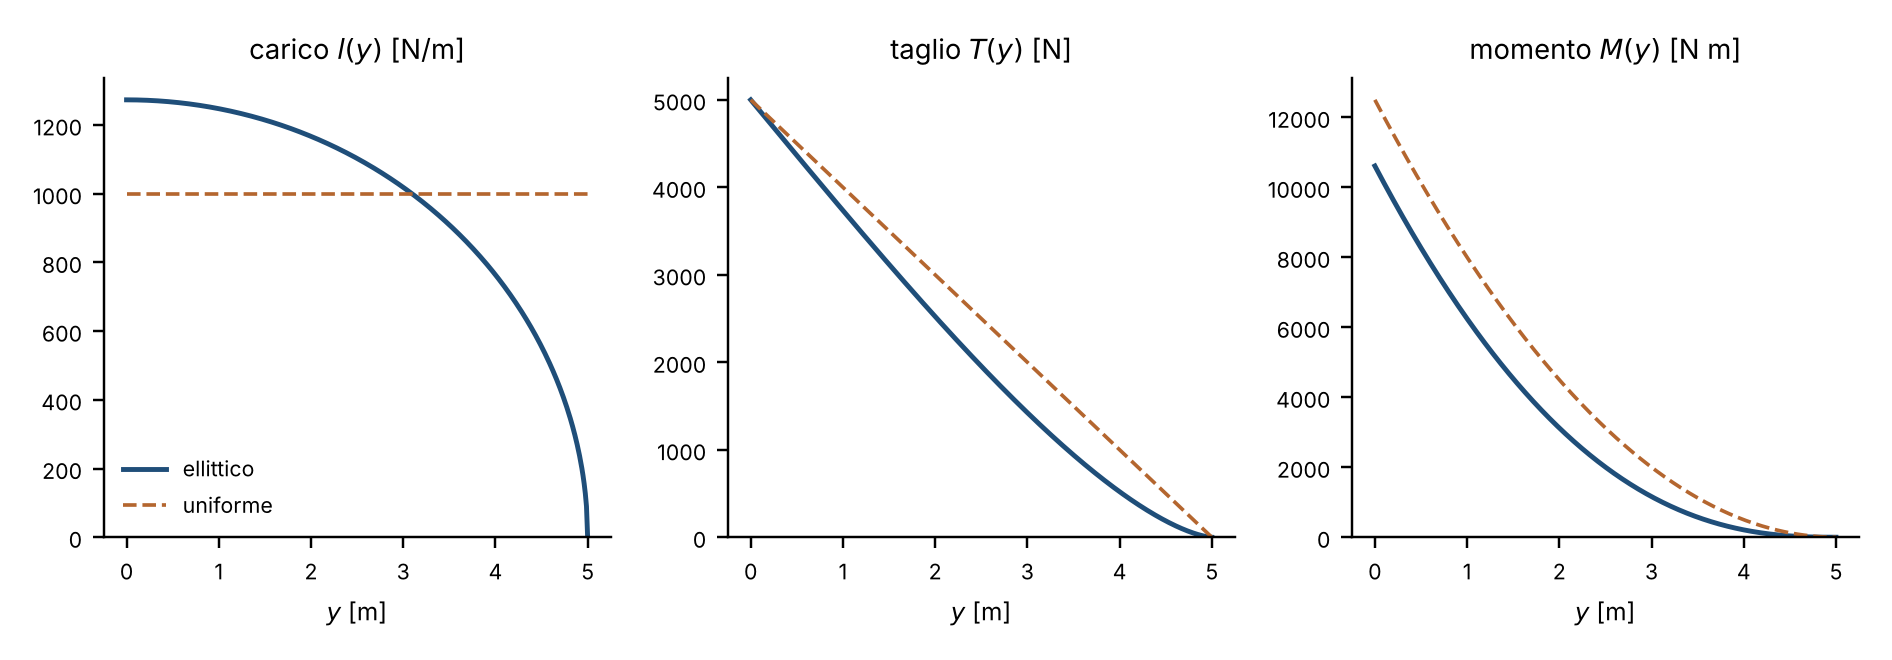
\includegraphics[width=\textwidth]{figure/taglio_momento.png}
\caption{Carico, taglio e momento flettente lungo la semiala per la distribuzione
ellittica ($W=10\,000$~N, $b=10$~m), confrontati con quelli di un carico uniforme con la
stessa portanza totale (tratteggio). Il taglio è l'area del carico all'esterno della
stazione, il momento l'area del taglio; le pendenze sono $T'=-l$ e $M'=-T$
(\texttt{python/fig\_taglio\_momento.py}).}
\label{fig:taglio-momento}
\end{figure}

Il programma seguente calcola il taglio e il momento numericamente, integrando il
carico dall'estremità verso la radice con la formula dei trapezi, e li confronta con le
formule \eqref{eq:taglio-ellittico} e \eqref{eq:momento-ellittico}.

\begin{python}[Taglio e momento flettente lungo la semiala]
import math

W, b = 10000.0, 10.0
s, l0 = b / 2, 4 * W / (math.pi * b)
l = lambda y: l0 * math.sqrt(max(0.0, 1 - (y / s)**2))

def T_esatto(y):
    u = y / s
    q = math.pi / 2 - math.asin(u) - u * math.sqrt(1 - u * u)
    return l0 * s / 2 * q

n = 5000                     # trapezi, dall'estremità alla radice
h = s / n
y = [s - k * h for k in range(n + 1)]
T, M = [0.0], [0.0]
for k in range(1, n + 1):
    T.append(T[-1] + h * (l(y[k - 1]) + l(y[k])) / 2)    # T' = -l
    M.append(M[-1] + h * (T[k - 1] + T[k]) / 2)          # M' = -T
print("  y [m]   T num. [N]  T esatto [N]   M num. [N m]")
for k in range(n, -1, -1000):
    print(f"{y[k]:6.1f}  {T[k]:10.1f}  {T_esatto(y[k]):11.1f}"
          f"  {M[k]:12.1f}")
print(f"M(0) esatto = W b/(3 pi) = {W * b / (3 * math.pi):.1f} N m")
\end{python}
\begin{risultato}
  y [m]   T num. [N]  T esatto [N]   M num. [N m]
   0.0      5000.0       5000.0       10610.3
   1.0      3735.3       3735.3        6244.8
   2.0      2523.2       2523.2        3122.3
   3.0      1423.8       1423.8        1161.1
   4.0       520.4        520.4         210.1
   5.0         0.0          0.0           0.0
M(0) esatto = W b/(3 pi) = 10610.3 N m
\end{risultato}

\begin{osservazione}[Un carico concentrato: il motore in ala]\label{oss:motore-ala}
Supponiamo che la semiala porti, oltre alla portanza $l$, il peso $P$ di un motore,
applicato nella stazione $y_{m}\in(0,s)$ e diretto verso il basso. Per $y<y_{m}$ il tratto
esterno $[y,s]$ comprende il motore, e le \eqref{eq:taglio-momento} diventano
\[
\begin{aligned}
  T(y)&=\int_{y}^{s}l(\eta)\,d\eta-P,\\
  M(y)&=\int_{y}^{s}(\eta-y)\,l(\eta)\,d\eta-P\,(y_{m}-y) \qquad (0\le y<y_{m}),
\end{aligned}
\]
mentre per $y\ge y_{m}$ restano invariate. Il taglio ha in $y_{m}$ un salto $P$; il
momento è continuo, ma ha in $y_{m}$ un punto angoloso, e $M'=-T$ vale soltanto per
$y\neq y_{m}$ (con la dimostrazione della \cref{prop:taglio-momento}). Dunque $M$ è
continua e regolare a tratti, e per il \cref{teo:formula-regolari-tratti}
$M(0)=-\int_{0}^{s}M'\,dy=\int_{0}^{s}T\,dy$: il momento alla radice è ancora l'area del
diagramma del taglio, mentre la stessa formula applicata al taglio, discontinuo,
sbaglierebbe di $P$ (\cref{oss:regolari-tratti-salti}). Si ha poi
$M(0)=\int_{0}^{s}y\,l(y)\,dy-P\,y_{m}$: il motore \emph{riduce} il momento alla radice, ed
è uno dei motivi per cui motori e combustibile si sistemano in ala. Con i dati
dell'\cref{es:taglio-ellittico}, $P=1000$~N e $y_{m}=1{,}5$~m, il momento scende da circa
$10\,610$ a circa $9\,110$~N\,m.
\end{osservazione}

\begin{notastorica}[Dalla trave di Galileo alle ali a sbalzo]
Il problema della resistenza di una trave incastrata a un estremo e caricata, la
\emph{mensola} o trave a sbalzo, fu posto da Galileo nei \emph{Discorsi e dimostrazioni
matematiche intorno a due nuove scienze} (1638), che lo risolse in modo errato quanto
alla distribuzione delle tensioni nella sezione. Le relazioni differenziali
$T'=-l$, $M'=-T$ e la teoria della flessione si consolidarono nel Settecento e
nell'Ottocento, con Jakob Bernoulli, Eulero e Navier. Tra le prime ali a sbalzo di impiego pratico, prive di
montanti e tiranti esterni, vi furono quelle realizzate da Hugo Junkers nel 1915 con il monoplano
metallico J~1: da allora il calcolo del taglio e del momento flettente lungo l'apertura,
cioè l'integrazione ripetuta della distribuzione di portanza, è il punto di partenza del
dimensionamento strutturale di ogni ala.
\end{notastorica}

%% ----------------------------------------------------------------------------
%%  §9.8  Appendice: integrali impropri
%% ----------------------------------------------------------------------------
\section{Appendice: integrali impropri}
\label{sec:impropri}

Nei paragrafi precedenti abbiamo studiato l'integrale definito di una funzione limitata
in un intervallo chiuso e limitato $[a,b]$. Nelle applicazioni è utile considerare anche
integrali come
\begin{equation}\label{eq:impropri-esempi}
  \int_{1}^{+\infty}\frac{dx}{x^{2}}, \qquad \int_{0}^{1}\frac{dx}{\sqrt x} .
\end{equation}
Tali integrali non rientrano nei casi trattati: nel primo l'intervallo di integrazione
è illimitato, nel secondo la funzione integranda non è limitata per $x\to0^{+}$. Integrali
di questo tipo si chiamano \emph{integrali impropri}.\index{integrale improprio} Come nel
testo di riferimento, ci limitiamo a funzioni \emph{continue} e \emph{non negative}
nell'intervallo considerato, e accenneremo al caso generale in un'osservazione.

\subsection{Intervalli illimitati}

Il punto di partenza è un fatto generale sulle funzioni monotòne, analogo al teorema
sulle successioni monotòne.

\begin{lemma}[Limite all'infinito di una funzione crescente]\label{lem:monotona-infinito}
Sia $F$ crescente in $[a,+\infty)$. Allora esiste il limite di $F(b)$ per $b\to+\infty$, ed è
uguale a $\sup\set{F(b) \tc b\ge a}$, finito se $F$ è limitata superiormente, $+\infty$ altrimenti.
\end{lemma}

\begin{schema}
\Ipotesi{$F$ crescente in $[a,+\infty)$.}
\Tesi{$\lim_{b\to+\infty}F(b)=\sup_{b\ge a}F(b)\in\R\cup\set{+\infty}$.}
\end{schema}

\begin{strategia}
È la stessa dimostrazione del teorema sulle successioni monotòne: un valore $F(b_{0})$
vicino all'estremo superiore si trova per la caratterizzazione dell'estremo superiore, e
la monotonia garantisce che tutti i valori successivi sono ancora più vicini.
\end{strategia}

\begin{dimostrazione}
Sia $\ell=\sup F$ finito e sia $\epsilon>0$. Per la \cref{prop:caratt-sup} esiste $b_{0}$ con
$F(b_{0})>\ell-\epsilon$; per $b>b_{0}$, la monotonia dà $\ell-\epsilon<F(b_{0})\le F(b)\le\ell$, cioè
$\abs{F(b)-\ell}<\epsilon$. Se invece $F$ non è limitata superiormente, per ogni $M$ esiste $b_{0}$
con $F(b_{0})>M$, e allora $F(b)>M$ per ogni $b>b_{0}$: $F(b)\to+\infty$.
\end{dimostrazione}

Sia ora $f$ continua e non negativa in $[a,+\infty)$, e sia $F(b)=\int_{a}^{b}f(x)\,dx$ per
$b\ge a$. Per l'additività e la positività dell'integrale, se $b_{1}<b_{2}$ si ha
$F(b_{2})-F(b_{1})=\int_{b_{1}}^{b_{2}}f\ge0$: $F$ è crescente (lo si vede anche dal teorema
fondamentale, perché $F'=f\ge0$). Per il lemma, esiste il limite di $F(b)$ per
$b\to+\infty$, ed è lecita la definizione seguente.

\begin{definizione}[Integrale improprio su un intervallo illimitato]
\label{def:improprio-illimitato}
Sia $f$ continua e non negativa in $[a,+\infty)$. Si pone
\begin{equation}\label{eq:improprio-illimitato}
  \int_{a}^{+\infty}f(x)\,dx=\lim_{b\to+\infty}\int_{a}^{b}f(x)\,dx .
\end{equation}
L'integrale improprio si dice \emph{convergente} se il limite è finito, \emph{divergente}
se il limite è $+\infty$.
\end{definizione}

In modo analogo si definisce l'integrale improprio di una funzione continua e non
negativa in $(-\infty,a]$, come limite per $b\to+\infty$ di $\int_{-b}^{a}f$, e in $(-\infty,+\infty)$,
come limite di $\int_{-b}^{b}f$. Per una funzione non negativa, quest'ultimo è convergente se e
solo se lo sono i due integrali su $(-\infty,0]$ e su $[0,+\infty)$, e ne è la somma.

\begin{esempio}[Gli integrali $\int_{1}^{+\infty}x^{-p}\,dx$]\label{es:impropri-p-infinito}
Per $p\neq1$, per la formula fondamentale,
\[
  \int_{1}^{b}\frac{dx}{x^{p}}=\Bigl[\frac{x^{1-p}}{1-p}\Bigr]_{1}^{b}=\frac{b^{1-p}}{1-p}+\frac1{p-1} ,
\]
e per $p=1$ si ha $\int_{1}^{b}\frac{dx}x=\log b$. Passando al limite per $b\to+\infty$,
\begin{equation}\label{eq:impropri-p-infinito}
  \int_{1}^{+\infty}\frac{dx}{x^{p}}=
  \begin{cases} \dfrac1{p-1} & \text{se } p>1,\\[4pt] +\infty & \text{se } p\le1 . \end{cases}
\end{equation}
In particolare $\int_{1}^{+\infty}\frac{dx}{x^{2}}=1$ (\cref{fig:impropri}, a sinistra): una regione
illimitata può avere area finita.
\end{esempio}

\begin{figure}[htb]
\centering
\begin{tikzpicture}
\begin{axis}[name=i1, width=0.52\textwidth, height=4.6cm, axis lines=middle,
  xmin=-0.2, xmax=8.4, ymin=-0.1, ymax=1.35, xtick={1,4,8}, ytick={1},
  title={\scriptsize $\int_{1}^{+\infty}x^{-2}dx=1$}, clip=false]
  \addplot[draw=none, fill=blu!22, domain=1:8.2, samples=80] {1/x^2} \closedcycle;
  \addplot[curva, domain=0.87:8.2, samples=80] {1/x^2};
  \addplot[curva2, dashed, domain=0.77:8.2, samples=80] {1/x};
  \node[font=\scriptsize, rame, anchor=south] at (axis cs:6.0,0.3) {$\frac1x$: area $+\infty$};
\end{axis}
\begin{axis}[at={(i1.east)}, anchor=west, xshift=0.7cm, width=0.46\textwidth,
  height=4.6cm, axis lines=middle, xmin=-0.1, xmax=1.25, ymin=-0.3, ymax=6.2,
  xtick={1}, ytick={1,5}, title={\scriptsize $\int_{0}^{1}x^{-1/2}dx=2$}]
  \addplot[draw=none, fill=blu!22, domain=0.026:1, samples=100] {1/sqrt(x)}
    \closedcycle;
  \addplot[curva, domain=0.026:1.2, samples=100] {1/sqrt(x)};
\end{axis}
\end{tikzpicture}
\caption{Due integrali impropri convergenti. A sinistra, la regione illimitata sotto
$\frac1{x^{2}}$ per $x\ge1$ ha area $1$, mentre quella sotto $\frac1x$ (tratteggio) ha area
infinita. A destra, la regione sotto $\frac1{\sqrt x}$ in $(0,1]$, illimitata verso l'alto, ha
area $2$.}
\label{fig:impropri}
\end{figure}

\begin{notastorica}[Il solido iperbolico acuto di Torricelli]
Che una figura illimitata possa avere misura finita fu una delle sorprese del Seicento.
Intorno al 1641 Evangelista Torricelli, che di lì a poco sarebbe succeduto a Galileo come
matematico del granduca di Toscana, studiò il solido generato dalla rotazione attorno
all'asse $x$ della regione sotto l'iperbole $y=\frac1x$, per $x\ge1$: un «corno»
infinitamente lungo, il \emph{solido iperbolico acuto}. Con gli indivisibili di Cavalieri
resi «curvi» (superfici cilindriche coassiali al posto delle sezioni piane) dimostrò che
il suo volume è uguale a quello di un cilindro finito, e pubblicò il risultato nel 1644,
nell'\emph{Opera geometrica}, con una seconda dimostrazione alla maniera di Archimede per
i lettori diffidenti verso gli indivisibili. In termini moderni, le sezioni
perpendicolari all'asse sono cerchi di area $\frac\pi{x^{2}}$, e il volume è
$\pi\int_{1}^{+\infty}\frac{dx}{x^{2}}=\pi$ per la \eqref{eq:impropri-p-infinito}, mentre la
superficie laterale è infinita, come lascia intuire il confronto con $\int_{1}^{+\infty}\frac{dx}x$.
Il risultato alimentò a lungo le discussioni filosofiche sull'infinito, come la polemica
tra Thomas Hobbes e John Wallis.
\end{notastorica}

Non sempre è possibile calcolare esplicitamente una primitiva. In tal caso può essere
utile il criterio seguente.

\begin{teorema}[Criterio del confronto]\label{teo:confronto-impropri}
\index{criterio!del confronto per gli integrali impropri}
Siano $f$ e $g$ continue in $[a,+\infty)$, con $0\le f(x)\le g(x)$ per ogni $x\ge a$. Se
l'integrale improprio di $g$ in $[a,+\infty)$ è convergente, anche quello di $f$ è
convergente, e $\int_{a}^{+\infty}f\le\int_{a}^{+\infty}g$. Se l'integrale di $f$ è divergente, anche
quello di $g$ è divergente.
\end{teorema}

\needspace{6\baselineskip}
\begin{schema}
\Ipotesi{$f$, $g$ continue in $[a,+\infty)$; \ $0\le f\le g$.}
\Tesi{$\int_{a}^{+\infty}g<+\infty\implica\int_{a}^{+\infty}f<+\infty$;\\
$\int_{a}^{+\infty}f=+\infty\implica\int_{a}^{+\infty}g=+\infty$.}
\end{schema}

\begin{strategia}
Il confronto vale per gli integrali su $[a,b]$, per ogni $b$; i due membri hanno limite per
$b\to+\infty$, e il confronto passa ai limiti.
\end{strategia}

\begin{dimostrazione}
Per il \cref{teo:confronto-integrali}, $\int_{a}^{b}f\le\int_{a}^{b}g$ per ogni $b>a$. Entrambi i membri
hanno limite per $b\to+\infty$; per il confronto dei limiti (\cref{teo:confronto-funzioni}),
il limite del primo membro non supera quello del secondo. Se il secondo è finito, lo è
anche il primo; se il primo è $+\infty$, lo è anche il secondo.
\end{dimostrazione}

\begin{esempio}[L'integrale di Gauss converge]\label{es:gauss-converge}
Verifichiamo che $\int_{0}^{+\infty}e^{-x^{2}}dx<+\infty$. L'integrale converge se e solo se converge
quello su $[1,+\infty)$, perché i due differiscono per l'integrale (finito) su $[0,1]$. Per
$x\ge1$ si ha $1\le x$ e, moltiplicando per $e^{-x^{2}}>0$,
\[
  e^{-x^{2}}\le x\,e^{-x^{2}} \qquad\perogni x\ge1 .
\]
La funzione a destra ha il vantaggio di avere una primitiva facilmente calcolabile, per
la \eqref{eq:integrali-composti}:
\[
  \int_{1}^{+\infty}x\,e^{-x^{2}}dx=\lim_{b\to+\infty}\Bigl[-\frac12e^{-x^{2}}\Bigr]_{1}^{b}
  =\lim_{b\to+\infty}\Bigl(\frac1{2e}-\frac12e^{-b^{2}}\Bigr)=\frac1{2e} .
\]
Per il criterio del confronto, l'integrale di $e^{-x^{2}}$ converge. Il suo valore,
$\int_{0}^{+\infty}e^{-x^{2}}dx=\frac{\sqrt\pi}2$, si calcola con gli integrali doppi (in un corso di Analisi
Matematica~2); qui lo verifichiamo numericamente. La convergenza appena dimostrata,
insieme alla parità di $e^{-x^{2}}$, giustifica gli asintoti orizzontali della funzione
integrale nella \cref{fig:funzione-integrale}: $F(x)=\int_{0}^{x}e^{-t^{2}}dt$ è crescente e
tende a un limite finito per $x\to+\infty$, e $F(-x)=-F(x)$.
\end{esempio}

\begin{esempio}[La velocità di fuga]\label{es:velocita-fuga}
Il lavoro necessario per vincere la forza di gravità $F(r)=\frac{GMm}{r^{2}}$ (l'opposto del
lavoro della forza peso) quando una massa $m$ si allontana dalla superficie terrestre
($r=R$) fino a una distanza $r_{1}$ è, come limite delle somme
$\sum F(r_{k})\,\Delta r_{k}$, l'integrale $\int_{R}^{r_{1}}\frac{GMm}{r^{2}}\,dr=GMm\bigl(\frac1R-\frac1{r_{1}}\bigr)$. Per
$r_{1}\to+\infty$ si ottiene l'integrale improprio convergente
\[
  \int_{R}^{+\infty}\frac{GMm}{r^{2}}\,dr=\frac{GMm}R=m\,g\,R ,
\]
dove $g=\frac{GM}{R^{2}}$ è l'accelerazione di gravità al suolo. Un corpo lanciato con velocità
$v$ sfugge all'attrazione terrestre (trascurando l'atmosfera) se la sua energia cinetica
$\frac12mv^{2}$ basta a compiere questo lavoro, cioè se $v\ge\sqrt{2gR}$: con $g=9{,}81$~m/s$^{2}$ e
$R=6371$~km si ottiene la velocità di fuga $\sqrt{2gR}\approx11{,}2$~km/s. Che il lavoro
per portare un corpo «all'infinito» sia finito dipende dal fatto che la forza decresce
come $r^{-2}$, cioè con esponente $p=2>1$ nella \eqref{eq:impropri-p-infinito}.
\end{esempio}

\subsection{Funzioni non limitate}

In modo analogo si procede per una funzione non limitata in prossimità di un estremo
dell'intervallo di integrazione, ad esempio dell'estremo $a$. Sia $f$ continua e non
negativa in $(a,b]$; per $0<h<b-a$ la funzione $h\mapsto\int_{a+h}^{b}f$ è decrescente (al crescere
di $h$ l'intervallo si restringe e la funzione integranda è non negativa), e quindi
esiste il limite per $h\to0^{+}$ (con la stessa dimostrazione del
\cref{lem:monotona-infinito}). Si pone
\begin{equation}\label{eq:improprio-non-limitata}
  \int_{a}^{b}f(x)\,dx=\lim_{h\to0^{+}}\int_{a+h}^{b}f(x)\,dx ,
\end{equation}
e l'integrale improprio si dice convergente se il limite è finito, divergente
altrimenti. Vale un criterio del confronto del tutto analogo al
\cref{teo:confronto-impropri}, con la stessa dimostrazione.

\begin{esempio}[Gli integrali $\int_{0}^{1}x^{-p}\,dx$]\label{es:impropri-p-zero}
Per $p\neq1$, $\int_{h}^{1}x^{-p}\,dx=\frac1{1-p}-\frac{h^{1-p}}{1-p}$, e per $p=1$ si ha
$\int_{h}^{1}\frac{dx}x=-\log h$. Passando al limite per $h\to0^{+}$,
\begin{equation}\label{eq:impropri-p-zero}
  \int_{0}^{1}\frac{dx}{x^{p}}=
  \begin{cases} \dfrac1{1-p} & \text{se } p<1,\\[4pt] +\infty & \text{se } p\ge1 . \end{cases}
\end{equation}
In particolare $\int_{0}^{1}\frac{dx}{\sqrt x}=2$ (\cref{fig:impropri}, a destra). Si noti che i ruoli di
$p>1$ e $p<1$ sono scambiati rispetto alla \eqref{eq:impropri-p-infinito}: all'infinito
conviene che la funzione decresca rapidamente, vicino a $0$ che cresca lentamente. Il
tempo di salita alla quota di tangenza teorica dell'\cref{es:tempo-salita},
$\int_{0}^{H}\frac{d\eta}{v_{z0}(1-\eta/H)}$, è un integrale di questo tipo nell'estremo $H$ (con
$p=1$, dopo la sostituzione $\eta=H-x$), e quindi diverge.
\end{esempio}

\begin{osservazione}[Funzioni di segno qualsiasi]\label{oss:convergenza-assoluta}
Se $f$ è continua in $[a,+\infty)$ ma cambia segno, la funzione $\int_{a}^{b}f$ non è più
monotòna e il suo limite può non esistere. Se però $\int_{a}^{+\infty}\abs f$ converge, si dice che
l'integrale di $f$ è \emph{assolutamente convergente}, e il limite
$\lim_{b\to+\infty}\int_{a}^{b}f$ esiste finito. Infatti le parti positiva e negativa
\eqref{eq:parte-positiva-negativa} verificano $0\le f^{\pm}\le\abs f$ e sono continue; per il
criterio del confronto i loro integrali convergono, e
$\int_{a}^{b}f=\int_{a}^{b}f^{+}-\int_{a}^{b}f^{-}$ tende alla differenza dei due limiti. Ad esempio,
$\int_{1}^{+\infty}\frac{\sen x}{x^{2}}\,dx$ converge assolutamente, perché
$\bigl|\frac{\sen x}{x^{2}}\bigr|\le\frac1{x^{2}}$. Esistono anche integrali convergenti ma non
assolutamente convergenti, come $\int_{0}^{+\infty}\frac{\sen x}x\,dx$, che studieremo nel
\S\ref{subsec:seno-su-x}.
\end{osservazione}

\begin{python}[Integrali impropri: verifiche numeriche]
import math

def punto_medio(f, a, b, n=200000):
    h = (b - a) / n
    return h * sum(f(a + (k + 0.5) * h) for k in range(n))

for B in (1, 2, 4, 6):
    I = punto_medio(lambda x: math.exp(-x * x), 0, B)
    print(f"int_0^{B} exp(-x^2) dx = {I:.10f}")
print(f"sqrt(pi)/2           = {math.sqrt(math.pi) / 2:.10f}")
for p in (0.5, 1, 2):
    v = [punto_medio(lambda x: x**-p, 1, B, 20000)
         for B in (10, 100, 1000)]
    print(f"p = {p}: int_1^B x^-p dx (B = 10, 100, 1000) =",
          ", ".join(f"{w:.3f}" for w in v))
g, R = 9.81, 6.371e6
print(f"velocità di fuga = {math.sqrt(2 * g * R) / 1000:.2f} km/s")
\end{python}
\begin{risultato}
int_0^1 exp(-x^2) dx = 0.7468241328
int_0^2 exp(-x^2) dx = 0.8820813908
int_0^4 exp(-x^2) dx = 0.8862269118
int_0^6 exp(-x^2) dx = 0.8862269255
sqrt(pi)/2           = 0.8862269255
p = 0.5: int_1^B x^-p dx (B = 10, 100, 1000) = 4.325, 18.000, 61.246
p = 1: int_1^B x^-p dx (B = 10, 100, 1000) = 2.303, 4.605, 6.908
p = 2: int_1^B x^-p dx (B = 10, 100, 1000) = 0.900, 0.990, 0.999
velocità di fuga = 11.18 km/s
\end{risultato}

\begin{notastorica}[L'integrale di Gauss]
L'integrale $\int_{-\infty}^{+\infty}e^{-x^{2}}dx=\sqrt\pi$ comparve per la prima volta nei lavori di Abraham
de Moivre (1733) sull'approssimazione della distribuzione binomiale, e il suo valore fu
poi stabilito da Laplace e da Gauss, che lo usò nel 1809 nella teoria degli errori di
misura legata al metodo dei minimi quadrati (\cref{sec:estremi-due}). Per questo la
funzione $e^{-x^{2}}$, opportunamente normalizzata, si chiama «gaussiana». Gli integrali
impropri, definiti come limiti di integrali ordinari, furono trattati sistematicamente
da Cauchy nelle lezioni del 1823.
\end{notastorica}

\subsection{Approfondimento: un integrale convergente ma non assolutamente convergente}
\label{subsec:seno-su-x}

Se $f$ è continua in $[a,+\infty)$ e ha segno qualsiasi, diciamo che l'integrale improprio
$\int_{a}^{+\infty}f(x)\,dx$ è \emph{convergente} se esiste finito il limite di $\int_{a}^{b}f$
per $b\to+\infty$, e indichiamo il limite con lo stesso simbolo. Per l'\cref{oss:convergenza-assoluta},
un integrale assolutamente convergente è convergente; il viceversa è falso, e l'esempio
classico è quello di $\frac{\sen x}x$, che, seguendo \cite{giusti}, possiamo studiare con i
soli strumenti di questo capitolo. Ci limitiamo all'intervallo $[1,+\infty)$: in $[0,1]$
la funzione $\frac{\sen x}x$, prolungata con il valore $1$ in $x=0$ (per il limite notevole
\eqref{eq:lim-senx-x}), è continua, e il suo integrale è un integrale ordinario.

\begin{proposizione}[L'integrale di $\frac{\sen x}x$]\label{prop:seno-su-x}
L'integrale improprio $\int_{1}^{+\infty}\frac{\sen x}x\,dx$ è convergente, ma non
assolutamente convergente: $\int_{1}^{+\infty}\frac{\abs{\sen x}}x\,dx=+\infty$.
\end{proposizione}

\begin{schema}
\Ipotesi{$f(x)=\frac{\sen x}x$, continua in $[1,+\infty)$.}
\Tesi{$\lim_{b\to+\infty}\int_{1}^{b}f$ esiste finito; \ $\int_{1}^{+\infty}\abs f=+\infty$.}
\end{schema}

\begin{strategia}
$\frac{\sen x}x$ decresce soltanto come $\frac1x$, che da solo non basterebbe; ma le
oscillazioni del seno producono compensazioni, che un'integrazione per parti rende
visibili, trasformando l'integrale in uno con $\frac{\cos x}{x^{2}}$, assolutamente
convergente. Per $\int\abs f$ si stima dal basso l'integrale su ogni arco
$[k\pi,(k+1)\pi]$ e si confronta la somma delle stime con $\int\frac{dt}t$, che diverge.
\end{strategia}

\begin{dimostrazione}
Per $b>1$, integrando per parti (\cref{teo:per-parti-definito}) con fattore finito
$\frac1x$ e fattore differenziale $\sen x$,
\begin{equation}\label{eq:seno-su-x-parti}
\begin{split}
  \int_{1}^{b}\frac{\sen x}x\,dx&=\Bigl[-\frac{\cos x}x\Bigr]_{1}^{b}
  -\int_{1}^{b}\frac{\cos x}{x^{2}}\,dx\\
  &=\cos1-\frac{\cos b}b-\int_{1}^{b}\frac{\cos x}{x^{2}}\,dx .
\end{split}
\end{equation}
Per $b\to+\infty$, $\frac{\cos b}b\to0$, perché $\abs{\cos b}\le1$; l'ultimo integrale ha limite
finito, perché $\bigl|\frac{\cos x}{x^{2}}\bigr|\le\frac1{x^{2}}$ e quindi converge assolutamente
(\cref{oss:convergenza-assoluta} e \eqref{eq:impropri-p-infinito} con $p=2$). Dunque il primo
membro ha limite finito.

Per la seconda affermazione, sia $k\in\N$. Con la sostituzione $x=u+k\pi$, poiché
$\abs{\sen(u+k\pi)}=\sen u$ per $u\in[0,\pi]$, si ha
$\int_{k\pi}^{(k+1)\pi}\abs{\sen x}\,dx=\int_{0}^{\pi}\sen u\,du=2$; inoltre
$\frac1x\ge\frac1{(k+1)\pi}$ per $x\le(k+1)\pi$. Per il confronto,
\[
  \int_{k\pi}^{(k+1)\pi}\frac{\abs{\sen x}}x\,dx\ge\frac2{(k+1)\pi}
  \ge\frac2\pi\int_{k+1}^{k+2}\frac{dt}t ,
\]
perché $\frac1t\le\frac1{k+1}$ in $[k+1,k+2]$. Sommando per $k=1,\dots,n$ e usando l'additività,
\[
  \int_{1}^{(n+1)\pi}\frac{\abs{\sen x}}x\,dx\ge\int_{\pi}^{(n+1)\pi}\frac{\abs{\sen x}}x\,dx
  \ge\frac2\pi\int_{2}^{n+2}\frac{dt}t=\frac2\pi\log\frac{n+2}2 ,
\]
che tende a $+\infty$. La funzione crescente $b\mapsto\int_{1}^{b}\frac{\abs{\sen x}}x\,dx$ non è
dunque limitata, e per il \cref{lem:monotona-infinito} tende a $+\infty$.
\end{dimostrazione}

Le compensazioni tra archi positivi e negativi sono decisive, come nelle serie a segni
alterni del \cref{cap:serie}. Il valore $\int_{0}^{+\infty}\frac{\sen x}x\,dx=\frac\pi2$ si
calcola in Analisi Matematica~2; il programma seguente lo verifica numericamente, con la
crescita logaritmica di $\int_{0}^{B}\frac{\abs{\sen x}}x\,dx$ prevista dalla dimostrazione.

\begin{python}[Convergenza semplice e divergenza assoluta]
import math

def punto_medio(f, a, b, n):
    h = (b - a) / n
    return h * sum(f(a + (k + 0.5) * h) for k in range(n))

f = lambda x: math.sin(x) / x
g = lambda x: abs(math.sin(x)) / x
print("    B   int_0^B sen x/x   int_0^B |sen x|/x   (2/pi) log B")
for B in (10, 100, 1000, 10000):
    I = punto_medio(f, 0, B, 100 * B)
    J = punto_medio(g, 0, B, 100 * B)
    L = 2 / math.pi * math.log(B)
    print(f"{B:5d}   {I:15.6f}   {J:17.6f}   {L:12.6f}")
print(f"pi/2 = {math.pi / 2:.6f}")
\end{python}
\begin{risultato}
    B   int_0^B sen x/x   int_0^B |sen x|/x   (2/pi) log B
   10          1.658348            2.558747       1.465871
  100          1.562225            4.046675       2.931742
 1000          1.570233            5.510356       4.397614
10000          1.570892            6.976394       5.863485
pi/2 = 1.570796
\end{risultato}

La prima colonna si stabilizza su $\frac\pi2$; la seconda differisce dall'ultima per circa
$1{,}11$: l'integrale di $\frac{\abs{\sen x}}x$ cresce come $\frac2\pi\log B$.

%% ----------------------------------------------------------------------------
%%  §9.9  Appendice: definizione di logaritmo, esponenziale, potenza
%% ----------------------------------------------------------------------------
\section{Appendice: logaritmo, esponenziale e potenza mediante un integrale}
\label{sec:logaritmo-integrale}

Nel \cref{cap:numeri} abbiamo introdotto le funzioni potenza, esponenziale e logaritmo a
partire dall'espressione $a^{b}$, appoggiandoci inizialmente all'idea intuitiva di
elevamento a potenza con esponente reale; nel \cref{cap:complementi} abbiamo dato un
significato rigoroso ad $a^{b}$ mediante l'estremo superiore. In questo paragrafo seguiamo
una strada diversa, basata sull'integrale definito: \emph{definiamo} il logaritmo come
una funzione integrale, e da esso deduciamo l'esponenziale e la potenza. Supponiamo
validi gli assiomi dei numeri reali, con il prodotto, il quoziente e le potenze $a^{n}$
con esponente naturale, e utilizziamo soltanto risultati dimostrati senza far uso delle
tre funzioni che vogliamo definire: in particolare, il numero $e$ definito come limite
della successione $\bigl(1+\frac1n\bigr)^{n}$ (\cref{teo:numero-e}), il teorema fondamentale, la
formula di sostituzione con una funzione lineare e i teoremi sulle funzioni monotòne e
sulle funzioni inverse.

La funzione $\frac1t$ è continua e decrescente per $t>0$. Poniamo, per $x>0$,
\begin{equation}\label{eq:L-definizione}
  L(x)=\int_{1}^{x}\frac{dt}t \qquad (x>0) .
\end{equation}
Per $x>1$, $L(x)$ è l'area sotto l'iperbole $y=\frac1t$ tra $1$ e $x$; per $0<x<1$ è l'opposto
dell'area tra $x$ e $1$ (\cref{fig:logaritmo-area}).

\begin{proposizione}[Proprietà della funzione $L$]\label{prop:L-proprieta}
La funzione $L$ definita dalla \eqref{eq:L-definizione} ha le proprietà seguenti.
\begin{enumerate}[label=\textup{(\alph*)}]
  \item $L$ è derivabile in $(0,+\infty)$ con $L'(x)=\frac1x$; è quindi continua e strettamente
  crescente, e $L(1)=0$.
  \item $L(x_{1}x_{2})=L(x_{1})+L(x_{2})$ per ogni $x_{1},x_{2}>0$; in particolare
  $L(x^{n})=n\,L(x)$ per ogni $n\in\N$ e $L\bigl(\frac1x\bigr)=-L(x)$.
  \item $L(e)=1$.
  \item $L$ è una biiezione di $(0,+\infty)$ su $\R$.
\end{enumerate}
\end{proposizione}

\needspace{9\baselineskip}
\begin{schema}
\Ipotesi{$L(x)=\int_{1}^{x}\frac{dt}t$ per $x>0$; \ $e=\lim\bigl(1+\frac1n\bigr)^{n}$.}
\Tesi{(a) $L'=\frac1x$, $L$ strettamente crescente, $L(1)=0$; \ (b) $L(x_{1}x_{2})=L(x_{1})+L(x_{2})$;
\ (c) $L(e)=1$; \ (d) $L:(0,+\infty)\to\R$ biiettiva.}
\end{schema}

\begin{strategia}
(a) è il teorema fondamentale. (b) è il cuore della questione: l'area sotto l'iperbole tra
$x_{1}$ e $x_{1}x_{2}$ è uguale a quella tra $1$ e $x_{2}$, perché la sostituzione $t=x_{1}s$ allarga
le basi di un fattore $x_{1}$ e riduce le altezze dello stesso fattore. (c) si ottiene
riconoscendo in $L\bigl((1+\frac1n)^{n}\bigr)=n\,L(1+\frac1n)$ un rapporto incrementale di $L$ in $1$. Per (d),
la (b) mostra che $L$ non è limitata né superiormente né inferiormente, e il teorema dei
valori intermedi fa il resto.
\end{strategia}

\begin{dimostrazione}
(a) Per il \cref{teo:fondamentale} (applicato in un intervallo chiuso contenuto in
$(0,+\infty)$ che contenga $1$ e abbia $x$ al suo interno), $L$ è derivabile con
$L'(x)=\frac1x>0$; per il
\cref{cor:derivata-positiva} è strettamente crescente, ed è continua perché derivabile.
Inoltre $L(1)=\int_{1}^{1}=0$.

(b) Fissati $x_{1},x_{2}>0$, per l'additività
\[
  L(x_{1}x_{2})=\int_{1}^{x_{1}x_{2}}\frac{dt}t=\int_{1}^{x_{1}}\frac{dt}t+\int_{x_{1}}^{x_{1}x_{2}}\frac{dt}t .
\]
Nell'ultimo integrale effettuiamo la sostituzione $t=g(s)=x_{1}s$, con $g'(s)=x_{1}$,
$g(1)=x_{1}$ e $g(x_{2})=x_{1}x_{2}$; per il \cref{teo:sostituzione-definita},
\[
  \int_{x_{1}}^{x_{1}x_{2}}\frac{dt}t=\int_{1}^{x_{2}}\frac{x_{1}\,ds}{x_{1}s}=\int_{1}^{x_{2}}\frac{ds}s=L(x_{2}) ,
\]
(se $x_{2}<1$ gli estremi sono in ordine decrescente, e le formule valgono per la
\eqref{eq:estremi-invertiti}), e quindi $L(x_{1}x_{2})=L(x_{1})+L(x_{2})$. Per induzione su $n$ si ottiene $L(x^{n})=nL(x)$; con
$x_{1}=x$, $x_{2}=\frac1x$ si ottiene $0=L(1)=L(x)+L\bigl(\frac1x\bigr)$.

(c) Sia $x_{n}=\bigl(1+\frac1n\bigr)^{n}$. Per la (b) e poiché $L(1)=0$,
\[
  L(x_{n})=n\,L\Bigl(1+\frac1n\Bigr)=\frac{L(1+\frac1n)-L(1)}{\frac1n} ,
\]
che è il rapporto incrementale di $L$ nel punto $1$ con incremento $\frac1n$; per la (a) esso
tende a $L'(1)=1$ (lungo la successione $h=\frac1n$, per la definizione stessa di limite di una
funzione, \cref{def:limite-funzione}). D'altra parte $x_{n}\to e$ e $L$ è continua, quindi $L(x_{n})\to L(e)$ (per la
\cref{prop:caratt-continuita}). Per l'unicità del limite, $L(e)=1$.

(d) Per la (a), $L$ è iniettiva. Poiché $L(2)>L(1)=0$, per la (b) si ha $L(2^{n})=nL(2)\to+\infty$
e $L(2^{-n})=-nL(2)\to-\infty$. Dato $y\in\R$, esistono quindi $n\in\N$ con $L(2^{-n})<y<L(2^{n})$, e
per il teorema dei valori intermedi (\cref{teo:valori-intermedi-2}), applicato alla funzione
continua $L$ nell'intervallo $[2^{-n},2^{n}]$, esiste $x$ con $L(x)=y$: $L$ è suriettiva su $\R$.
\end{dimostrazione}

\begin{figure}[htb]
\centering
\begin{tikzpicture}
\begin{axis}[name=g1, width=0.5\textwidth, height=4.6cm, axis lines=middle,
  xmin=-0.1, xmax=4.4, ymin=-0.1, ymax=2.3, xtick={1,3}, xticklabels={$1$,$x$},
  ytick={1}, title={\scriptsize $L(x)=\int_{1}^{x}\frac{dt}t$}]
  \addplot[draw=none, fill=blu!22, domain=1:3, samples=50] {1/x} \closedcycle;
  \addplot[curva, domain=0.45:4.3, samples=100] {1/x};
  \node[font=\scriptsize, blu] at (axis cs:1.9,0.22) {$L(x)$};
\end{axis}
\begin{axis}[at={(g1.east)}, anchor=west, xshift=0.7cm, width=0.5\textwidth,
  height=4.6cm, axis lines=middle, xmin=-0.1, xmax=4.4, ymin=-0.1, ymax=1.3,
  xtick={1,1.5,2.5,3.75}, xticklabels={$1$,$x_{2}$,$x_{1}$,$x_{1}x_{2}$},
  ytick=\empty, title={\scriptsize aree uguali: $L(x_{1}x_{2})-L(x_{1})=L(x_{2})$},
  tick label style={font=\scriptsize}]
  \addplot[draw=none, fill=blu!22, domain=1:1.5, samples=40] {1/x} \closedcycle;
  \addplot[draw=none, fill=rame!30, domain=2.5:3.75, samples=40] {1/x} \closedcycle;
  \addplot[curva, domain=0.8:4.3, samples=100] {1/x};
\end{axis}
\end{tikzpicture}
\caption{A sinistra, il logaritmo come area sotto l'iperbole. A destra, la regione tra
$1$ e $x_{2}$ e quella tra $x_{1}$ e $x_{1}x_{2}$ (qui $x_{1}=2{,}5$, $x_{2}=1{,}5$) hanno la stessa area: la
seconda si ottiene dalla prima allargando le basi di un fattore $x_{1}$ e riducendo le
altezze dello stesso fattore. È la proprietà $L(x_{1}x_{2})=L(x_{1})+L(x_{2})$.}
\label{fig:logaritmo-area}
\end{figure}

Per la \cref{prop:L-proprieta}(d), la funzione $L$ è invertibile. Indichiamo con
$E:\R\to(0,+\infty)$ la funzione inversa, definita da
\begin{equation}\label{eq:E-definizione}
  E(y)=x \quad\sse\quad L(x)=y .
\end{equation}

\needspace{9\baselineskip}
\begin{proposizione}[Proprietà della funzione $E$]\label{prop:E-proprieta}
La funzione $E$ è continua, strettamente crescente e derivabile in $\R$, con
\begin{equation}\label{eq:E-proprieta}
\begin{gathered}
  E'(y)=E(y), \qquad E(0)=1, \qquad E(1)=e,\\
  E(y_{1}+y_{2})=E(y_{1})\,E(y_{2}) .
\end{gathered}
\end{equation}
Inoltre, per ogni $a>0$ e $n\in\N$, $E\bigl(n\,L(a)\bigr)=a^{n}$.
\end{proposizione}

\begin{schema}
\Ipotesi{$E=L^{-1}:\R\to(0,+\infty)$.}
\Tesi{$E$ continua, strettamente crescente, $E'=E$; \ $E(0)=1$, $E(1)=e$;
\ $E(y_{1}+y_{2})=E(y_{1})E(y_{2})$; \ $E(nL(a))=a^{n}$.}
\end{schema}

\begin{strategia}
Le proprietà di regolarità passano dalla funzione alla sua inversa per i teoremi sulle
funzioni inverse. Le identità algebriche si ottengono applicando $L$, che è iniettiva, a
entrambi i membri e usando la \cref{prop:L-proprieta}.
\end{strategia}

\begin{dimostrazione}
In ogni intervallo chiuso $[\alpha,\beta]\subset(0,+\infty)$ la funzione $L$ è continua e strettamente
crescente; per i \cref{teo:continuita-inversa,teo:derivata-inversa} la sua inversa è
continua e strettamente crescente in $[L(\alpha),L(\beta)]$, e derivabile con
$E'(y)=\frac1{L'(E(y))}=E(y)$. Poiché ogni $y\in\R$ è interno a un intervallo di questo tipo,
le proprietà valgono in tutto $\R$. Da $L(1)=0$ e $L(e)=1$ seguono $E(0)=1$ ed $E(1)=e$. Posto
$x_{i}=E(y_{i})$, per la \cref{prop:L-proprieta}(b) $L(x_{1}x_{2})=y_{1}+y_{2}$, cioè
$E(y_{1}+y_{2})=x_{1}x_{2}=E(y_{1})E(y_{2})$. Infine $L(a^{n})=nL(a)$, cioè $E(nL(a))=a^{n}$.
\end{dimostrazione}

L'identità $a^{n}=E\bigl(n\,L(a)\bigr)$ esprime la potenza a esponente naturale mediante
$E$ e $L$, e suggerisce come definire la potenza con esponente reale.

\begin{definizione}[Potenza con esponente reale]\label{def:potenza-integrale}
Se $a$ e $x$ sono numeri reali, con $a>0$, si pone
\begin{equation}\label{eq:potenza-integrale}
  a^{x}=E\bigl(x\,L(a)\bigr) .
\end{equation}
\end{definizione}

La definizione è coerente con quella elementare: per $x=n\in\N$ restituisce $a^{n}$ (per la
\cref{prop:E-proprieta}); per $x=\frac mn$, con $m,n\in\N$, il numero $a^{m/n}$ così definito è
positivo e verifica, per la \eqref{eq:E-proprieta},
$\bigl(a^{m/n}\bigr)^{n}=E\bigl(\frac mnL(a)\bigr)^{n}=E\bigl(mL(a)\bigr)=a^{m}$, cioè è la radice $n$-esima
positiva di $a^{m}$, come nella \eqref{eq:potenza-razionale}. Inoltre $E(0)=1=a^{0}$ e,
poiché $E(y)\,E(-y)=E(0)=1$, si ha $a^{-m/n}=E\bigl(-\frac mnL(a)\bigr)=\frac1{a^{m/n}}$, ancora in
accordo con la \eqref{eq:potenza-razionale}. Le due funzioni $x\mapsto E(xL(a))$ e $x\mapsto a^{x}$
(quella del \cref{cap:complementi}, continua per il \cref{teo:continuita-esponenziale})
sono continue in $\R$ e coincidono sui razionali; poiché ogni numero reale $x$ è limite di
una successione di razionali (basta scegliere $q_{k}\in\Q\cap(x-\frac1k,x)$, che esiste per il
\cref{teo:densita-Q}), per la \cref{prop:caratt-continuita} esse coincidono ovunque. In particolare, per $a=e$,
poiché $L(e)=1$, si ha la \emph{funzione esponenziale}
\begin{equation}\label{eq:esponenziale-integrale}
  e^{x}=E(x) ,
\end{equation}
e, poiché il logaritmo naturale è la funzione inversa di $e^{x}$,
\begin{equation}\label{eq:logaritmo-integrale}
  \log x=L(x)=\int_{1}^{x}\frac{dt}t \qquad (x>0) .
\end{equation}
Risultano così definite le funzioni potenza, esponenziale e logaritmo, e si riconosce
facilmente che esse godono delle proprietà illustrate nel \cref{cap:numeri}. Ad esempio,
$\log(x_{1}x_{2})=\log x_{1}+\log x_{2}$ è la \cref{prop:L-proprieta}(b), che applicata a
$\frac{x_{1}}{x_{2}}$ e $x_{2}$ dà $\log\frac{x_{1}}{x_{2}}=\log x_{1}-\log x_{2}$.

\begin{python}[Il logaritmo come area e l'esponenziale come sua inversa]
import math

def L(x, n=100000):
    """L(x) = int_1^x dt/t, formula del punto medio."""
    h = (x - 1) / n
    return h * sum(1 / (1 + (k + 0.5) * h) for k in range(n))

def E(y):
    """Inversa di L, per bisezione (L è crescente)."""
    a, b = 1e-6, 1e6
    for _ in range(80):
        m = math.sqrt(a * b)            # bisezione «geometrica»
        a, b = (m, b) if L(m, 2000) < y else (a, m)
    return math.sqrt(a * b)

for x in (0.5, 2, 3, 6, math.e):
    print(f"L({x:.4f}) = {L(x):.8f}   log = {math.log(x):.8f}")
print(f"L(2) + L(3) = {L(2) + L(3):.8f} = L(6)")
for y in (-1, 1, 2):
    print(f"E({y:2d}) = {E(y):.5f}   exp = {math.exp(y):.5f}")
\end{python}
\begin{risultato}
L(0.5000) = -0.69314718   log = -0.69314718
L(2.0000) = 0.69314718   log = 0.69314718
L(3.0000) = 1.09861229   log = 1.09861229
L(6.0000) = 1.79175947   log = 1.79175947
L(2.7183) = 1.00000000   log = 1.00000000
L(2) + L(3) = 1.79175947 = L(6)
E(-1) = 0.36788   exp = 0.36788
E( 1) = 2.71828   exp = 2.71828
E( 2) = 7.38906   exp = 7.38906
\end{risultato}

Nella funzione \texttt{E} la bisezione sostituisce a ogni passo il rapporto $b/a$ tra gli
estremi con la sua radice quadrata, invece di dimezzarne la differenza, perché l'intervallo di partenza $[10^{-6},10^{6}]$ copre
molti ordini di grandezza; per contenere i tempi di calcolo vi si usa una formula meno
precisa per $L$ ($n=2000$), e stampiamo soltanto cinque decimali, che bastano a
riconoscere $e^{-1}$, $e$ ed $e^{2}$.

\begin{notastorica}[Il logaritmo e l'iperbole]
Che le aree sotto l'iperbole si comportino come logaritmi fu scoperto prima che si
conoscessero il calcolo integrale e il numero $e$. La proprietà (a)
della \cref{prop:L-proprieta} era già, in un certo senso, nella definizione cinematica di
Nepero (1614): un punto percorre un segmento con velocità uguale alla distanza che gli
resta da percorrere, un altro si muove con velocità costante, e il logaritmo della
distanza residua del primo è lo spazio percorso dal secondo; la velocità di variazione
del logaritmo è quindi inversamente proporzionale al numero. Il gesuita Grégoire de Saint-Vincent
mostrò nel 1647 che, se le ascisse crescono in progressione geometrica, le aree
corrispondenti sotto l'iperbole crescono in progressione aritmetica (è la nostra
\cref{fig:logaritmo-area}); il suo allievo Alphonse Antonio de Sarasa ne dedusse nel 1649
che tali aree hanno le proprietà dei logaritmi. Nicolaus Mercator, nella
\emph{Logarithmotechnia} (1668), calcolò l'area sotto $\frac1{1+t}$ sviluppandola in serie e
ottenne $\log(1+x)=x-\frac{x^{2}}2+\frac{x^{3}}3-\cdots$, da lui chiamato «logaritmo naturale».
In quale base fossero questi logaritmi «iperbolici», come furono chiamati per tutto il
Settecento, lo chiarì Eulero nell'\emph{Introductio in analysin infinitorum} (1748),
definendo il logaritmo come inverso dell'esponenziale: la base è $e$, come dice la (c)
della \cref{prop:L-proprieta}.
L'impostazione di questo paragrafo, che fa del logaritmo una funzione integrale, è
quella adottata da molti trattati moderni, perché rende immediate la derivabilità e la
proprietà fondamentale del logaritmo.
\end{notastorica}

%% ----------------------------------------------------------------------------
%%  §9.10  Esercizi di riepilogo
%% ----------------------------------------------------------------------------
\section{Esercizi di riepilogo}
\label{sec:esercizi-cap9}

Come nei capitoli precedenti, ogni soluzione è accompagnata da una nota sulla
\emph{scelta logica} che la guida.

\needspace{8\baselineskip}
\subsection*{Teorema fondamentale e funzioni integrali}

\begin{esercizio}
Calcolare la derivata di $G(x)=\int_{x}^{x^{2}}e^{-t^{2}}\,dt$.
\begin{soluzione}
Per l'additività, $G(x)=\int_{0}^{x^{2}}e^{-t^{2}}dt-\int_{0}^{x}e^{-t^{2}}dt$, e per il
\cref{cor:estremi-variabili} $G'(x)=2x\,e^{-x^{4}}-e^{-x^{2}}$. \emph{Scelta logica:} quando
entrambi gli estremi variano, si spezza l'integrale in un punto fisso, riducendosi a due
funzioni integrali; non serve (e non sarebbe possibile) calcolare una primitiva di
$e^{-t^{2}}$.
\end{soluzione}
\end{esercizio}

\begin{esercizio}
Determinare i punti di massimo e di minimo relativo di
$F(x)=\int_{0}^{x}(t^{2}-1)\,e^{-t^{2}}\,dt$.
\begin{soluzione}
Per il teorema fondamentale $F'(x)=(x^{2}-1)\,e^{-x^{2}}$, che è negativa in $(-1,1)$ e positiva
fuori. Per il criterio di monotonia, $F$ cresce in $(-\infty,-1]$, decresce in $[-1,1]$ e cresce
in $[1,+\infty)$: $x=-1$ è punto di massimo relativo, $x=1$ di minimo relativo.
\emph{Scelta logica:} della funzione integrale si conosce la derivata, e lo studio della
monotonia si fa come per qualsiasi funzione derivabile.
\end{soluzione}
\end{esercizio}

\begin{esercizio}
Calcolare $\displaystyle\lim_{x\to0}\frac1{x^{3}}\int_{0}^{x}\sen(t^{2})\,dt$.
\begin{soluzione}
Numeratore e denominatore tendono a $0$; il numeratore è derivabile con derivata
$\sen(x^{2})$, per il teorema fondamentale. Per il teorema di L'Hôpital
(\cref{teo:hopital}) il limite è quello di $\frac{\sen(x^{2})}{3x^{2}}$, che vale $\frac13$ per il limite
notevole \eqref{eq:lim-senx-x}. \emph{Scelta logica:} il teorema fondamentale permette di
applicare il teorema di L'Hôpital a quozienti in cui compare una funzione integrale; il risultato
dice che $\int_{0}^{x}\sen(t^{2})\,dt\approx\frac{x^{3}}3$ per $x$ piccolo, come se $\sen(t^{2})$ fosse $t^{2}$.
\end{soluzione}
\end{esercizio}

\needspace{8\baselineskip}
\subsection*{Calcolo di integrali}

\begin{esercizio}
Calcolare (a) $\int\frac{e^{2x}}{1+e^{2x}}\,dx$; \ (b) $\int\sen^{3}x\,dx$; \ (c) $\int\frac{dx}{x^{2}+4}$; \
(d) $\int\frac{3x+1}{x^{2}-4}\,dx$.
\begin{soluzione}
(a) Il numeratore è metà della derivata del denominatore: l'integrale è
$\frac12\log(1+e^{2x})+c$. (b) Si scrive $\sen^{3}x=\sen x\,(1-\cos^{2}x)$; poiché $\sen x=-D\cos x$,
$\int\sen^{3}x\,dx=-\cos x+\frac{\cos^{3}x}3+c$. (c) Per la \eqref{eq:argomento-lineare},
$\frac1{x^{2}+4}=\frac14\cdot\frac1{1+(x/2)^{2}}$, e l'integrale è $\frac12\operatorname{arctg}\frac x2+c$. (d) Le radici
del denominatore sono $\pm2$; per la \eqref{eq:fratti-semplici-distinte} con $x_{1}=2$,
$x_{2}=-2$, $A=\frac74$, $B=\frac54$, e l'integrale è $\frac74\log\abs{x-2}+\frac54\log\abs{x+2}+c$.
\emph{Scelta logica:} prima di ogni metodo generale conviene cercare la derivata di una
funzione «interna» (a, b), o un'arcotangente con argomento lineare (c); il metodo dei
fratti semplici è sistematico ma più lungo.
\end{soluzione}
\end{esercizio}

\begin{esercizio}\label{es:wallis}
(a) Calcolare $\int x^{2}e^{x}\,dx$. (b) Dimostrare che, per $n\ge2$,
$I_{n}=\int_{0}^{\pi/2}\sen^{n}x\,dx$ verifica $I_{n}=\frac{n-1}n\,I_{n-2}$, e calcolare $I_{2}$, $I_{3}$, $I_{4}$.
\begin{soluzione}
(a) Per parti due volte, con fattore finito $x^{2}$ e poi $x$:
$\int x^{2}e^{x}dx=x^{2}e^{x}-2\int xe^{x}dx=(x^{2}-2x+2)\,e^{x}+c$. (b) Per parti con fattore finito
$\sen^{n-1}x$ e fattore differenziale $\sen x$:
\[
\begin{aligned}
  I_{n}&=\Bigl[-\sen^{n-1}x\cos x\Bigr]_{0}^{\pi/2}
  +(n-1)\int_{0}^{\pi/2}\sen^{n-2}x\cos^{2}x\,dx\\
  &=(n-1)\,(I_{n-2}-I_{n}) ,
\end{aligned}
\]
perché il termine finito si annulla in entrambi gli estremi e $\cos^{2}x=1-\sen^{2}x$. Quindi
$nI_{n}=(n-1)I_{n-2}$. Con $I_{0}=\frac\pi2$ e $I_{1}=1$: $I_{2}=\frac\pi4$, $I_{3}=\frac23$, $I_{4}=\frac{3\pi}{16}$.
\emph{Scelta logica:} quando l'integrazione per parti riproduce un integrale dello
stesso tipo con esponente più basso, si ottiene una \emph{formula di riduzione}; da
questa si ricava il celebre prodotto infinito per $\pi$, che John Wallis aveva ottenuto
nel 1656, nell'\emph{Arithmetica infinitorum}, con un procedimento di interpolazione.
\end{soluzione}
\end{esercizio}

\begin{esercizio}
Calcolare (a) $\int_{0}^{1}x\sqrt{1-x^{2}}\,dx$; \ (b) $\int\frac{dx}{e^{x}+e^{-x}}$.
\begin{soluzione}
(a) Con la sostituzione $w=1-x^{2}$, $dw=-2x\,dx$, che porta $x=0$ in $w=1$ e $x=1$ in $w=0$:
$\int_{0}^{1}x\sqrt{1-x^{2}}\,dx=\frac12\int_{0}^{1}\sqrt w\,dw=\frac13$. (b) Moltiplicando numeratore e
denominatore per $e^{x}$, $\frac1{e^{x}+e^{-x}}=\frac{e^{x}}{1+e^{2x}}$, e con $u=e^{x}$, $du=e^{x}dx$:
$\int\frac{du}{1+u^{2}}=\operatorname{arctg}e^{x}+c$. \emph{Scelta logica:} in (a) il fattore $x$ è,
a meno di una costante, la derivata di $1-x^{2}$: la sostituzione $w=1-x^{2}$ elimina la radice
senza introdurre funzioni trigonometriche; nella forma definita gli estremi si
trasformano e non occorre tornare alla variabile $x$. In (b) l'integranda è una funzione
razionale di $e^{x}$, e la sostituzione $u=e^{x}$ la trasforma in una funzione razionale di $u$.
\end{soluzione}
\end{esercizio}

\needspace{8\baselineskip}
\subsection*{Aree, valori medi, applicazioni}

\begin{esercizio}
Calcolare l'area della regione compresa tra i grafici di $\sen x$ e $\cos x$ in
$[\frac\pi4,\frac{5\pi}4]$.
\begin{soluzione}
In questo intervallo $\sen x\ge\cos x$ (le due funzioni si incontrano agli estremi), e per la
\eqref{eq:area-tra-curve} l'area è
$\int_{\pi/4}^{5\pi/4}(\sen x-\cos x)\,dx=\bigl[-\cos x-\sen x\bigr]_{\pi/4}^{5\pi/4}
=\sqrt2+\sqrt2=2\sqrt2$. \emph{Scelta logica:} prima di integrare si stabilisce quale delle
due funzioni è maggiore; se si scambiassero nel corso dell'intervallo, occorrerebbe
spezzarlo nei punti di intersezione.
\end{soluzione}
\end{esercizio}

\begin{esercizio}
La rete elettrica di bordo di molti velivoli è in corrente alternata a $400$~Hz, con
tensione $v(t)=V_{0}\sen\omega t$. Il \emph{valore efficace} è la radice della media integrale
di $v^{2}$ su un periodo $[0,\frac{2\pi}\omega]$. Calcolarlo, e ricavare $V_{0}$ per una rete da $115$~V
efficaci.
\begin{soluzione}
Con la sostituzione $x=\omega t$ e la \eqref{eq:integrale-sen2},
\[
\begin{aligned}
  \frac\omega{2\pi}\int_{0}^{2\pi/\omega}V_{0}^{2}\sen^{2}\omega t\,dt
  &=\frac{V_{0}^{2}}{2\pi}\int_{0}^{2\pi}\sen^{2}x\,dx\\
  &=\frac{V_{0}^{2}}{2\pi}\Bigl[\frac{x-\sen x\cos x}2\Bigr]_{0}^{2\pi}=\frac{V_{0}^{2}}2 ,
\end{aligned}
\]
quindi il valore efficace è $\frac{V_{0}}{\sqrt2}$, e per $115$~V efficaci la tensione di picco è
$V_{0}=115\sqrt2\approx162{,}6$~V. \emph{Scelta logica:} la potenza dissipata in un resistore è
proporzionale a $v^{2}$; il valore efficace è la tensione continua che dissiperebbe la
stessa potenza media, e la media integrale è lo strumento giusto per definirlo.
\end{soluzione}
\end{esercizio}

\begin{esercizio}
Un gas perfetto viene compresso a temperatura costante dal volume $V_{1}$ al volume $V_{2}<V_{1}$.
Calcolare il lavoro $\int_{V_{2}}^{V_{1}}p\,dV$ necessario, e valutarlo per $1$~m$^{3}$ d'aria a
$101\,325$~Pa compresso a metà volume.
\begin{soluzione}
Per la legge di Boyle, $pV=p_{1}V_{1}$ è costante, quindi $p=\frac{p_{1}V_{1}}V$ e
$\int_{V_{2}}^{V_{1}}\frac{p_{1}V_{1}}V\,dV=p_{1}V_{1}\log\frac{V_{1}}{V_{2}}$. Con i dati,
$101\,325\cdot\log2\approx70\,200$~J, cioè circa $70$~kJ. \emph{Scelta logica:} il lavoro di una forza
variabile è un integrale (come nell'\cref{es:velocita-fuga}); poiché $p$ è proporzionale a
$\frac1V$, compare il logaritmo. È la legge di Boyle (temperatura costante),
la stessa che governa l'atmosfera isoterma del \cref{cap:applicazioni-derivate}
(\cref{es:atmosfera-isoterma}).
\end{soluzione}
\end{esercizio}

\begin{esercizio}
Calcolare taglio e momento flettente lungo la semiala per un carico uniforme
$l(y)=\frac Wb$, $0\le y\le s=\frac b2$, e confrontare il momento alla radice con quello della
distribuzione ellittica.
\begin{soluzione}
Per le \eqref{eq:taglio-momento}, $T(y)=\frac Wb(s-y)$; poiché $M'=-T$ e $M(s)=0$
(\cref{prop:taglio-momento}), $M(y)=\int_{y}^{s}T=\frac W{2b}(s-y)^{2}$; alla
radice $T(0)=\frac W2$ e $M(0)=\frac{Ws^{2}}{2b}=\frac{Wb}8$. Il rapporto con il momento ellittico
\eqref{eq:momento-ellittico} è $\frac{Wb/(3\pi)}{Wb/8}=\frac8{3\pi}\approx0{,}85$. \emph{Scelta logica:}
il taglio è lineare e il momento parabolico, come prevedono le relazioni $T'=-l$ e $M'=-T$
con $l$ costante: ogni integrazione aumenta di uno il grado del polinomio.
\end{soluzione}
\end{esercizio}

\needspace{8\baselineskip}
\subsection*{Integrali impropri e logaritmo}

\begin{esercizio}
Stabilire il carattere e, se possibile, calcolare: (a) $\int_{0}^{+\infty}x\,e^{-x}\,dx$; \
(b) $\int_{0}^{+\infty}\frac{dx}{1+x^{2}}$; \ (c) $\int_{2}^{+\infty}\frac{dx}{x\log x}$; \ (d) $\int_{2}^{+\infty}\frac{dx}{x\log^{2}x}$.
\begin{soluzione}
(a) Per parti, $\int_{0}^{b}xe^{-x}dx=\bigl[-(x+1)e^{-x}\bigr]_{0}^{b}=1-(b+1)e^{-b}\to1$, perché
$\frac{b+1}{e^{b}}\to0$ (per il teorema di L'Hôpital, \cref{teo:hopital}): converge e vale
$1$.
(b) $\int_{0}^{b}\frac{dx}{1+x^{2}}=\operatorname{arctg}b\to\frac\pi2$ \eqref{eq:arctg-infinito}. (c) Una primitiva è
$\log(\log x)$, che tende a $+\infty$: diverge. (d) Una primitiva è $-\frac1{\log x}$, e
$\int_{2}^{b}=\frac1{\log2}-\frac1{\log b}\to\frac1{\log2}$: converge. \emph{Scelta logica:} quando
si conosce una primitiva, si calcola l'integrale su $[a,b]$ e si passa al limite per
$b\to+\infty$, come vuole la definizione. Gli integrali (c) e (d) mostrano che il confine
tra convergenza e divergenza è sottile: un fattore $\log x$ in più al denominatore basta a
far convergere l'integrale, pur crescendo $\log x$ più lentamente di qualsiasi potenza.
\end{soluzione}
\end{esercizio}

\begin{esercizio}
Usando la \eqref{eq:logaritmo-integrale}, dimostrare che $\frac{x-1}x\le\log x\le x-1$ per ogni
$x>0$.
\begin{soluzione}
Sia $x>1$. Per $t\in[1,x]$ si ha $\frac1x\le\frac1t\le1$, e per il confronto
$\frac{x-1}x\le\int_{1}^{x}\frac{dt}t\le x-1$. Se $0<x<1$, per $t\in[x,1]$ si ha $1\le\frac1t\le\frac1x$, quindi
$1-x\le\int_{x}^{1}\frac{dt}t\le\frac{1-x}x$; cambiando segno, $\frac{x-1}x\le\log x\le x-1$. Per $x=1$ i tre
membri sono nulli. \emph{Scelta logica:} definito il logaritmo come area, le
disuguaglianze si ottengono confrontando l'area sotto l'iperbole con quelle di due
rettangoli; ritroviamo, per altra via, la disuguaglianza
dell'\cref{es:disuguaglianze-exp-log}.
\end{soluzione}
\end{esercizio}

Il programma seguente verifica con \texttt{sympy} alcuni risultati degli esercizi.

\begin{python}[Verifiche simboliche degli esercizi]
import sympy as sp

x, t = sp.symbols("x t", real=True)
G = sp.integrate(sp.exp(-t**2), (t, x, x**2))
print("G'(x) =", sp.simplify(sp.diff(G, x)))
lim = sp.limit(sp.integrate(sp.sin(t**2), (t, 0, x)) / x**3, x, 0)
print("lim =", sp.gammasimp(lim))
print("int x^2 e^x =", sp.factor(sp.integrate(x**2 * sp.exp(x), x)))
I = [sp.integrate(sp.sin(x)**n, (x, 0, sp.pi / 2)) for n in range(5)]
print("I_0..I_4 =", I)
print("int_0^oo x e^-x =",
      sp.integrate(x * sp.exp(-x), (x, 0, sp.oo)))
print("int_2^oo 1/(x log^2 x) =",
      sp.integrate(1 / (x * sp.log(x)**2), (x, 2, sp.oo)))
\end{python}
\begin{risultato}
G'(x) = 2*x*exp(-x**4) - exp(-x**2)
lim = 1/3
int x^2 e^x = (x**2 - 2*x + 2)*exp(x)
I_0..I_4 = [pi/2, 1, pi/4, 2/3, 3*pi/16]
int_0^oo x e^-x = 1
int_2^oo 1/(x log^2 x) = 1/log(2)
\end{risultato}

%% ----------------------------------------------------------------------------
%%  §9.11  Punti fondamentali del capitolo
%% ----------------------------------------------------------------------------
\section{Punti fondamentali del capitolo}
\label{sec:sintesi-cap09}

Integrazione e derivazione sono operazioni inverse: la funzione integrale di una
funzione continua ne è una primitiva, e un integrale definito si calcola come differenza
dei valori di una primitiva negli estremi. Il calcolo degli integrali diventa così la
ricerca delle primitive, per la quale bastano poche tecniche generali, ciascuna figlia di
una regola di derivazione.

\begin{puntichiave}
\item \textbf{Funzione integrale.} Se $f$ è integrabile in $[a,b]$ e $\abs f\le K$, la
funzione $F(x)=\int_{a}^{x}f(t)\,dt$ è lipschitziana con costante $K$, quindi continua
(\cref{prop:integrale-lipschitz}); può però non essere derivabile: un salto di $f$
diventa un punto angoloso di $F$.
\item \textbf{Teorema fondamentale.} Se $f$ è continua in $[a,b]$, allora $F$ è
derivabile e $F'(x)=f(x)$ per ogni $x\in[a,b]$ (\cref{teo:fondamentale}); se $f$ è soltanto
integrabile, basta la continuità in un punto $x_{0}$ per avere $F'(x_{0})=f(x_{0})$
(\cref{oss:fondamentale-puntuale}). Con la regola della
catena, $\frac{d}{dx}\int_{c}^{\varphi(x)}f(t)\,dt=f(\varphi(x))\,\varphi'(x)$
(\cref{cor:estremi-variabili}).
\item \textbf{Primitive.} Ogni funzione continua in un intervallo ha primitive; in un
intervallo due primitive della stessa funzione differiscono per una costante
(\cref{teo:caratterizzazione-primitive}). Fuori dagli intervalli la tesi è falsa: su
$\R\setminus\set{0}$ la costante può cambiare tra $x<0$ e $x>0$.
\item \textbf{Formula fondamentale.} Se $f$ è continua in $[a,b]$ e $G'=f$, allora
$\int_{a}^{b}f(x)\,dx=G(b)-G(a)$ (\cref{teo:formula-fondamentale}); la formula vale anche
per $f$ soltanto integrabile, purché dotata di primitiva
(\cref{oss:formula-fondamentale-integrabili}).
\item \textbf{Integrale indefinito.} $\int f(x)\,dx=F(x)+c$ indica l'insieme delle
primitive in un intervallo (\cref{def:integrale-indefinito}): è un insieme di funzioni,
non un numero. Si calcola con la linearità, gli integrali immediati
(\cref{tab:integrali-immediati}) e la regola $\int g(\varphi(x))\,\varphi'(x)\,dx
=G(\varphi(x))+c$.
\item \textbf{Funzioni razionali.} Si divide il numeratore per il denominatore e si
scompone il resto in fratti semplici; con denominatore di secondo grado si ottengono
logaritmi se $\Delta>0$, un termine $-\frac{mx_{1}+n}{x-x_{1}}$ se $\Delta=0$, un logaritmo e
un'arcotangente se $\Delta<0$ (\cref{prop:razionali-secondo-grado}).
\item \textbf{Integrazione per parti.} Se $f$ e $g$ hanno derivata continua,
$\int fg'\,dx=fg-\int f'g\,dx$ (\cref{teo:per-parti}), e negli integrali definiti compare
il termine $\bigl[fg\bigr]_{a}^{b}$ (\cref{teo:per-parti-definito}). Come fattore finito
si sceglie una funzione che si semplifica derivando; talvolta ricompare l'integrale di
partenza, o uno dello stesso tipo (formule di riduzione).
\item \textbf{Integrazione per sostituzione.} Se $f$ è continua e $g$ ha derivata
continua, $F\circ g$ è una primitiva di $(f\circ g)\,g'$ (\cref{teo:sostituzione}); negli
integrali definiti $\int_{a}^{b}f(x)\,dx=\int_{c}^{d}f(g(t))\,g'(t)\,dt$ con $g(c)=a$,
$g(d)=b$, senza che $g$ debba essere invertibile (\cref{teo:sostituzione-definita}).
\item \textbf{Errori da evitare.} Una primitiva vale in un intervallo: $\int\frac{dx}x
=\log\abs x+c$, non $\log x+c$, e i programmi di calcolo simbolico omettono spesso il valore
assoluto. Non tutte le funzioni integrabili hanno primitive (la funzione che vale $-1$ per
$x<0$ e $1$ per $x\ge0$ non ne ha, per il lemma di Darboux), e le primitive di $e^{-x^{2}}$ o
di $\frac{\sen x}x$ esistono ma non sono elementari.
\item \textbf{Aree.} La regione compresa tra i grafici di $g\le f$ continue in $[a,b]$ ha
area $\int_{a}^{b}(f-g)\,dx$ \eqref{eq:area-tra-curve}; con le sostituzioni $x=\sen t$ e
$x=rt$ si ottengono l'area $\pi r^{2}$ del cerchio e l'area $\pi ab$ dell'ellisse
(\cref{es:cerchio-ellisse}).
\item \textbf{Taglio e momento flettente.} Per un carico $l$ continuo sulla semiala,
$T'=-l$, $M'=-T$, $T(s)=M(s)=0$ e $M(0)=\int_{0}^{s}y\,l(y)\,dy$
(\cref{prop:taglio-momento}); la distribuzione ellittica dà $M(0)=\frac{Wb}{3\pi}$, circa il
$15\%$ in meno del carico uniforme (\cref{es:taglio-ellittico}). Integrando si ricavano
anche il tempo di salita e la legge della pressione nella troposfera standard
(\cref{es:tempo-salita,es:pressione-isa}).
\item \textbf{Integrali impropri.} Per $f$ continua e non negativa in $[a,+\infty)$,
l'integrale improprio $\int_{a}^{+\infty}f$, limite di $\int_{a}^{b}f$ per $b\to+\infty$, esiste
sempre, finito o $+\infty$ (\cref{def:improprio-illimitato}); $\int_{1}^{+\infty}x^{-p}\,dx$ converge se e solo se
$p>1$, $\int_{0}^{1}x^{-p}\,dx$ se e solo se $p<1$
(\cref{es:impropri-p-infinito,es:impropri-p-zero}), e il criterio del confronto
(\cref{teo:confronto-impropri}) prova, ad esempio, la convergenza di
$\int_{0}^{+\infty}e^{-x^{2}}dx$.
\item \textbf{Il logaritmo come integrale.} Posto $L(x)=\int_{1}^{x}\frac{dt}t$ per $x>0$,
si ha $L'=\frac1x$, $L(x_{1}x_{2})=L(x_{1})+L(x_{2})$, $L(e)=1$, e $L$ è una biiezione di
$(0,+\infty)$ su $\R$ (\cref{prop:L-proprieta}); la sua inversa $E$ verifica $E'=E$
(\cref{prop:E-proprieta}), e $a^{x}=E(x\,L(a))$ ritrova la potenza a esponente reale
(\cref{def:potenza-integrale}).
\end{puntichiave}

\paragraph{Il filo del discorso.} Il calcolo integrale ci ha dato un modo nuovo di
rappresentare una funzione di classe $C^{1}$: come integrale della sua derivata,
$f(x)=f(x_{0})+\int_{x_{0}}^{x}f'(t)\,dt$. Nel \cref{cap:taylor} integreremo ripetutamente
per parti questa identità, ottenendo la formula di Taylor con il resto integrale e con il
resto di Lagrange, che permettono di \emph{stimare} l'errore delle approssimazioni
polinomiali; la stessa formula, applicata al momento flettente di questo capitolo, darà
la freccia di un'ala a sbalzo.

